\documentclass{beamer}
\usetheme{default}

\title{CRISPR Screen}
\subtitle{Unsupervised Clustering with Automated Hyperparameter Selection}
\author{Keira Wiechecki}
\date{\today}

\begin{document}
\frame{
	\titlepage
}

\frame{
	\frametitle{Rationale}
	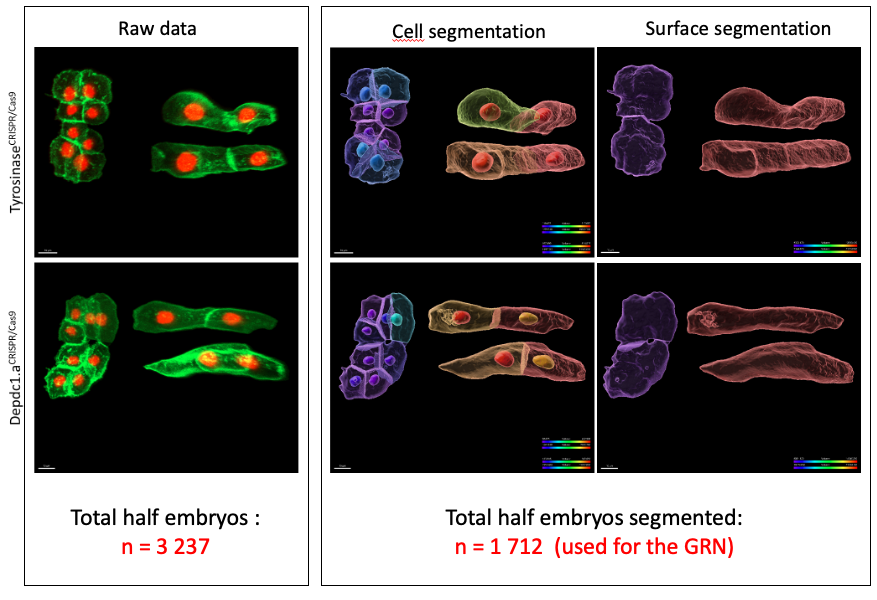
\includegraphics[width=\textwidth]{flowchart/segmentation.png}
}

\frame{
	\frametitle{Overview}
	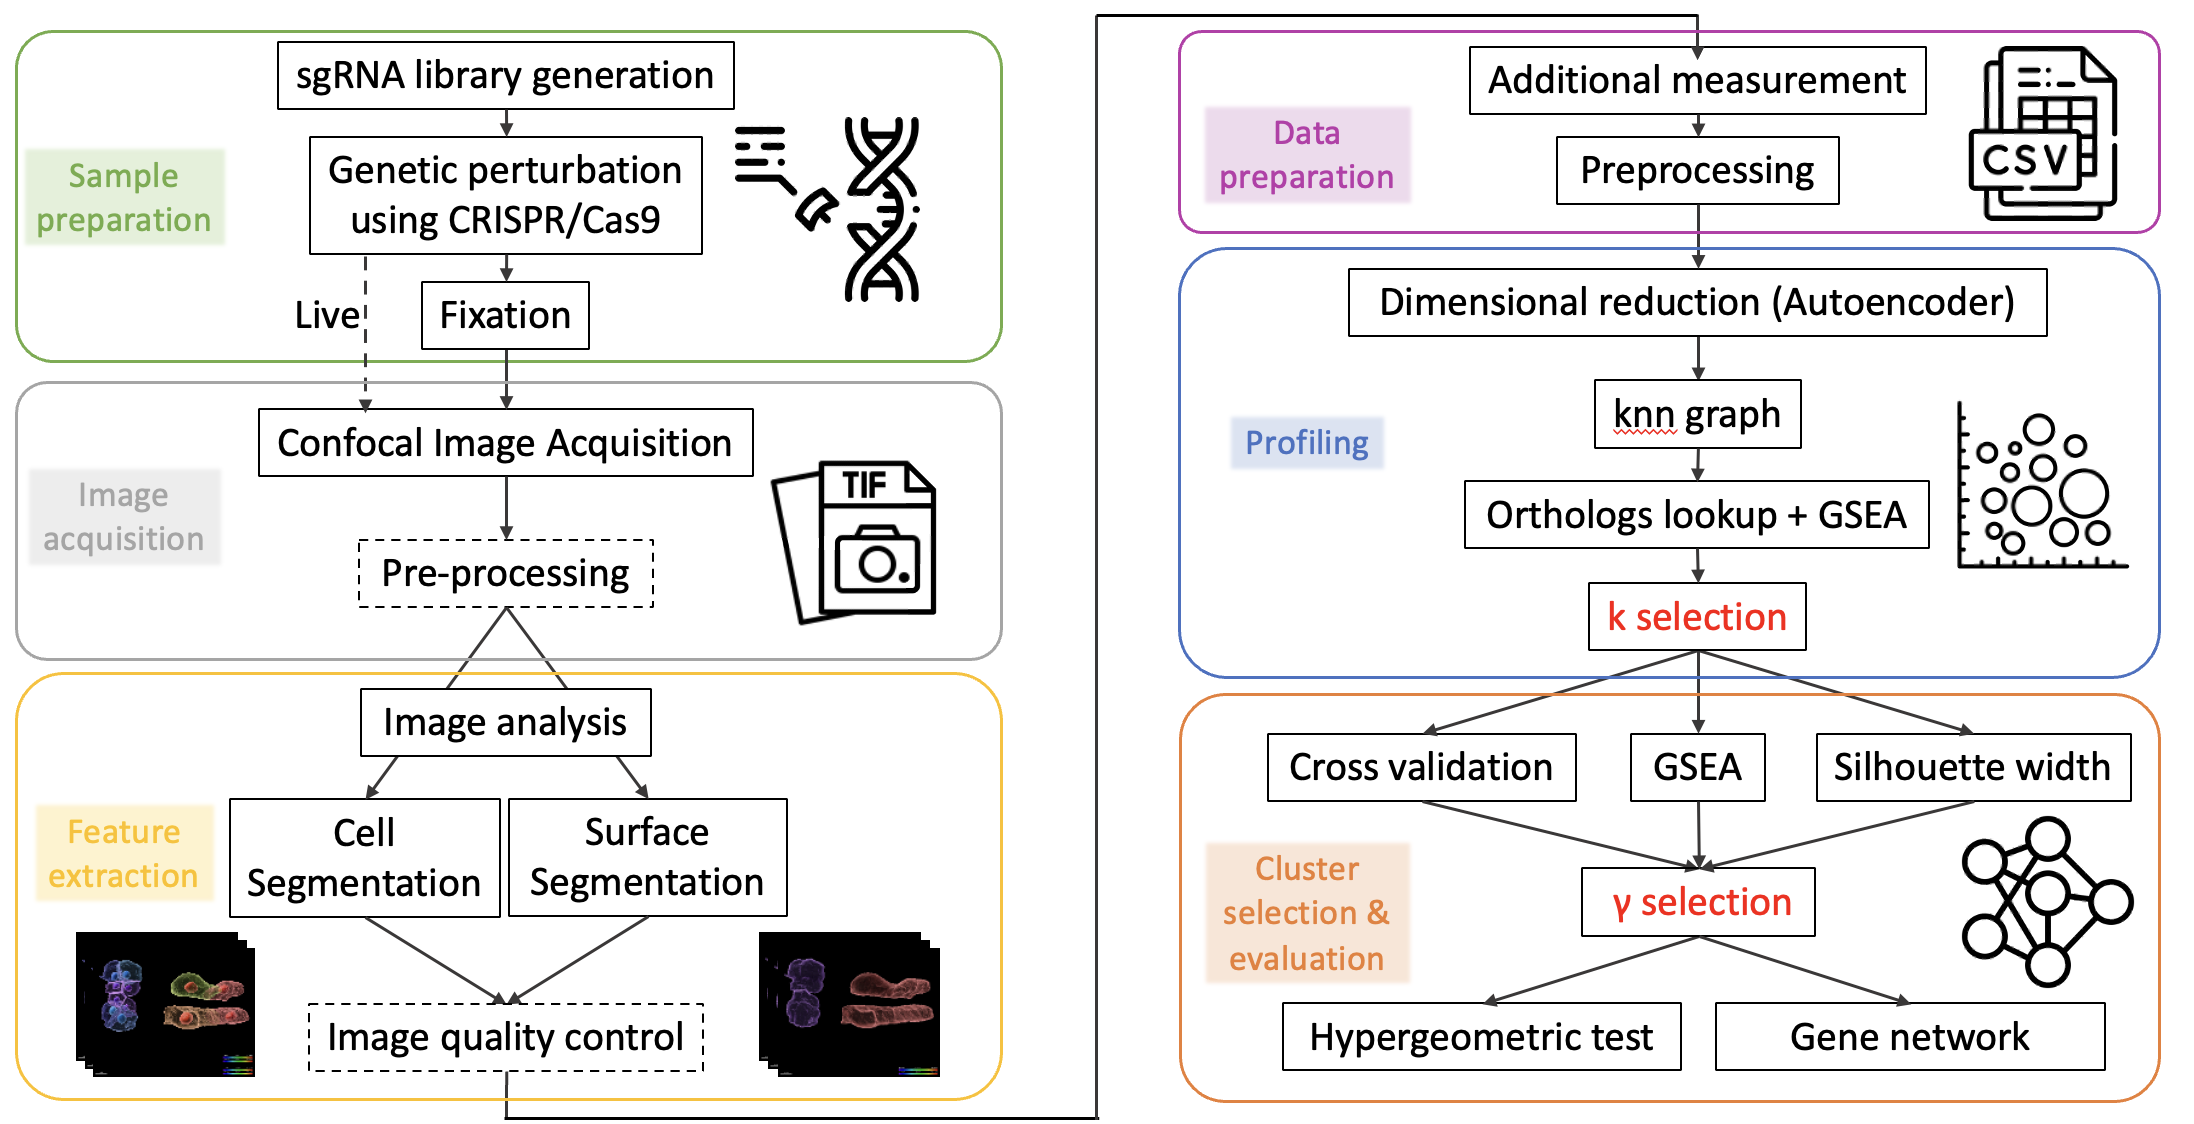
\includegraphics[width=\textwidth]{flowchart/overview.png}
}
\frame{
	\frametitle{}
	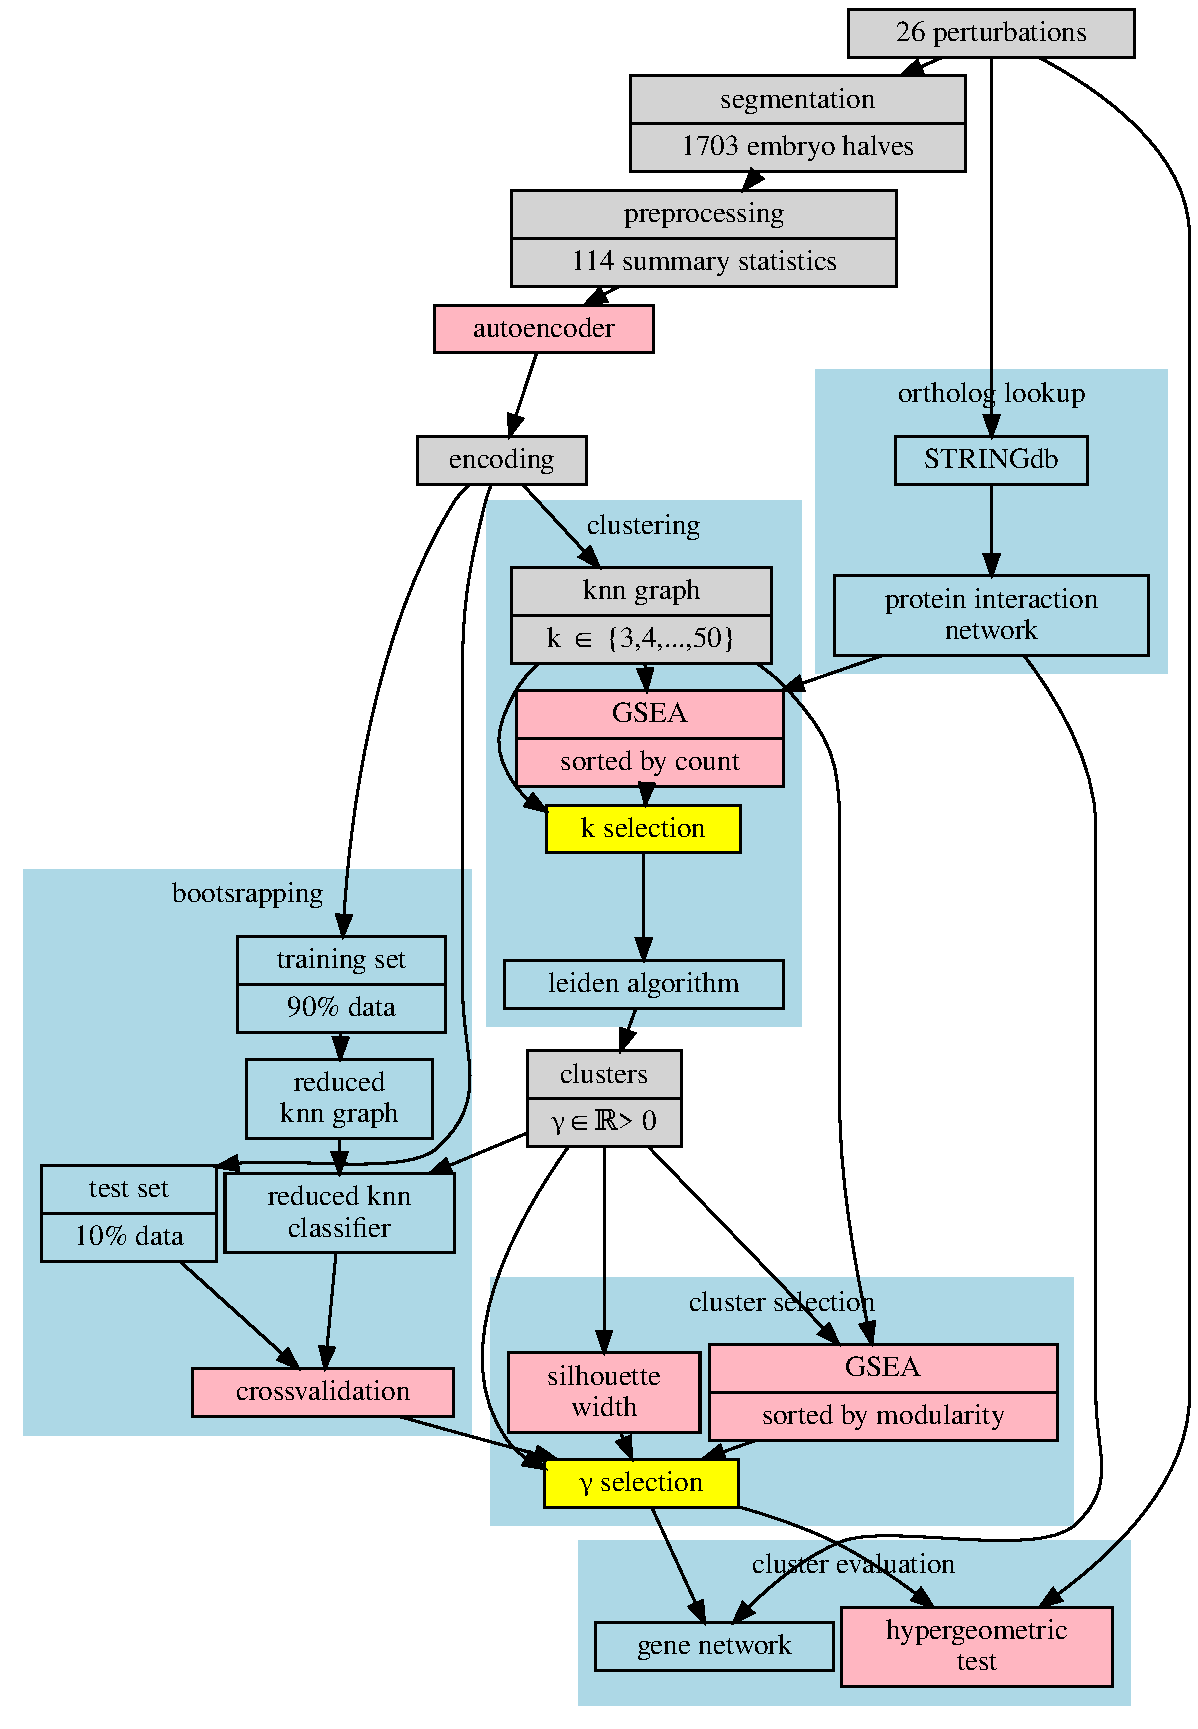
\includegraphics[height=\textheight]{flowchart/flowchart.pdf}
}

\frame{
	\frametitle{}
	\begin{columns}
		\begin{column}{0.50\textwidth}
			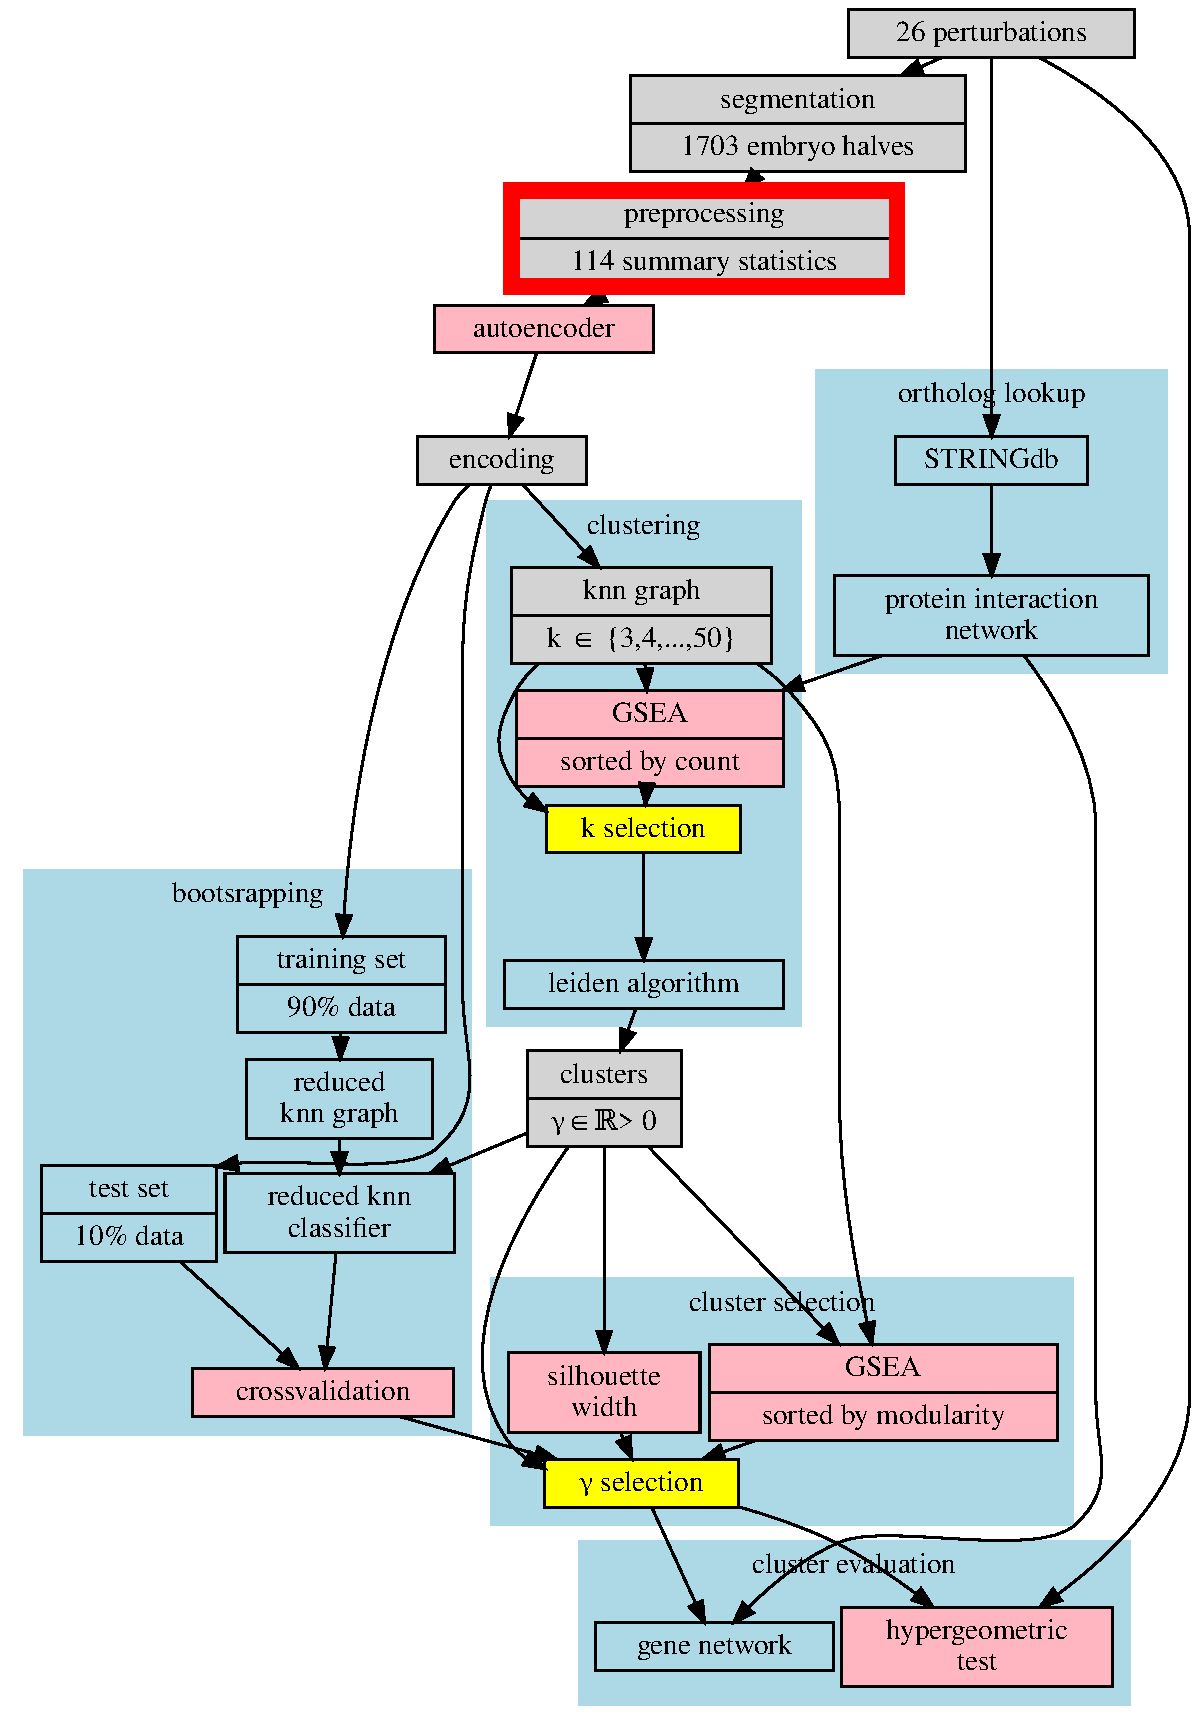
\includegraphics[width=\textwidth]{flowchart/preprocessing.pdf}
		\end{column}
		\begin{column}{0.50\textwidth}
			From the segmentation summary statistics I computed 114 embryo-level parameters. Parameters were normalized by z-score then scaled between -1 and 1.
		\end{column}
	\end{columns}
}

\frame{
	\frametitle{}
	\begin{columns}
		\begin{column}{0.40\textwidth}
			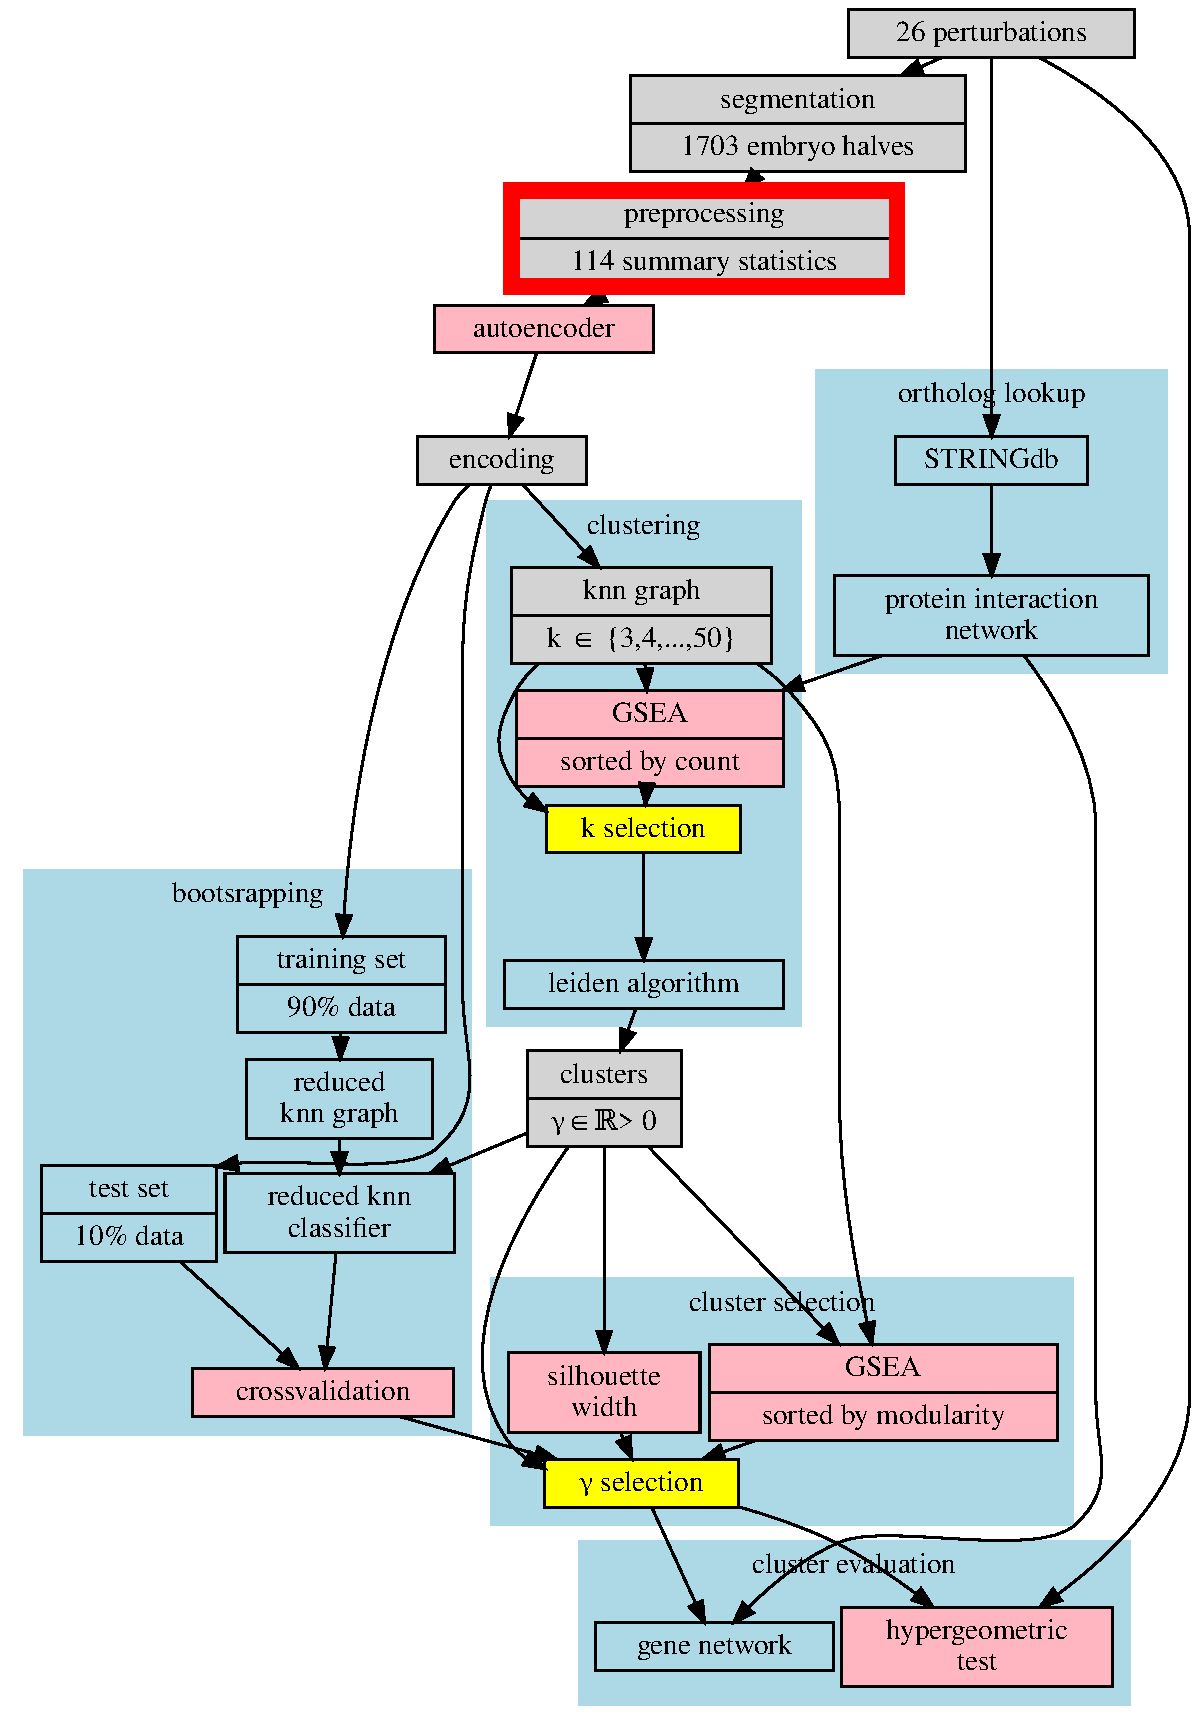
\includegraphics[width=\textwidth]{flowchart/preprocessing.pdf}
		\end{column}
		\begin{column}{0.80\textwidth}
			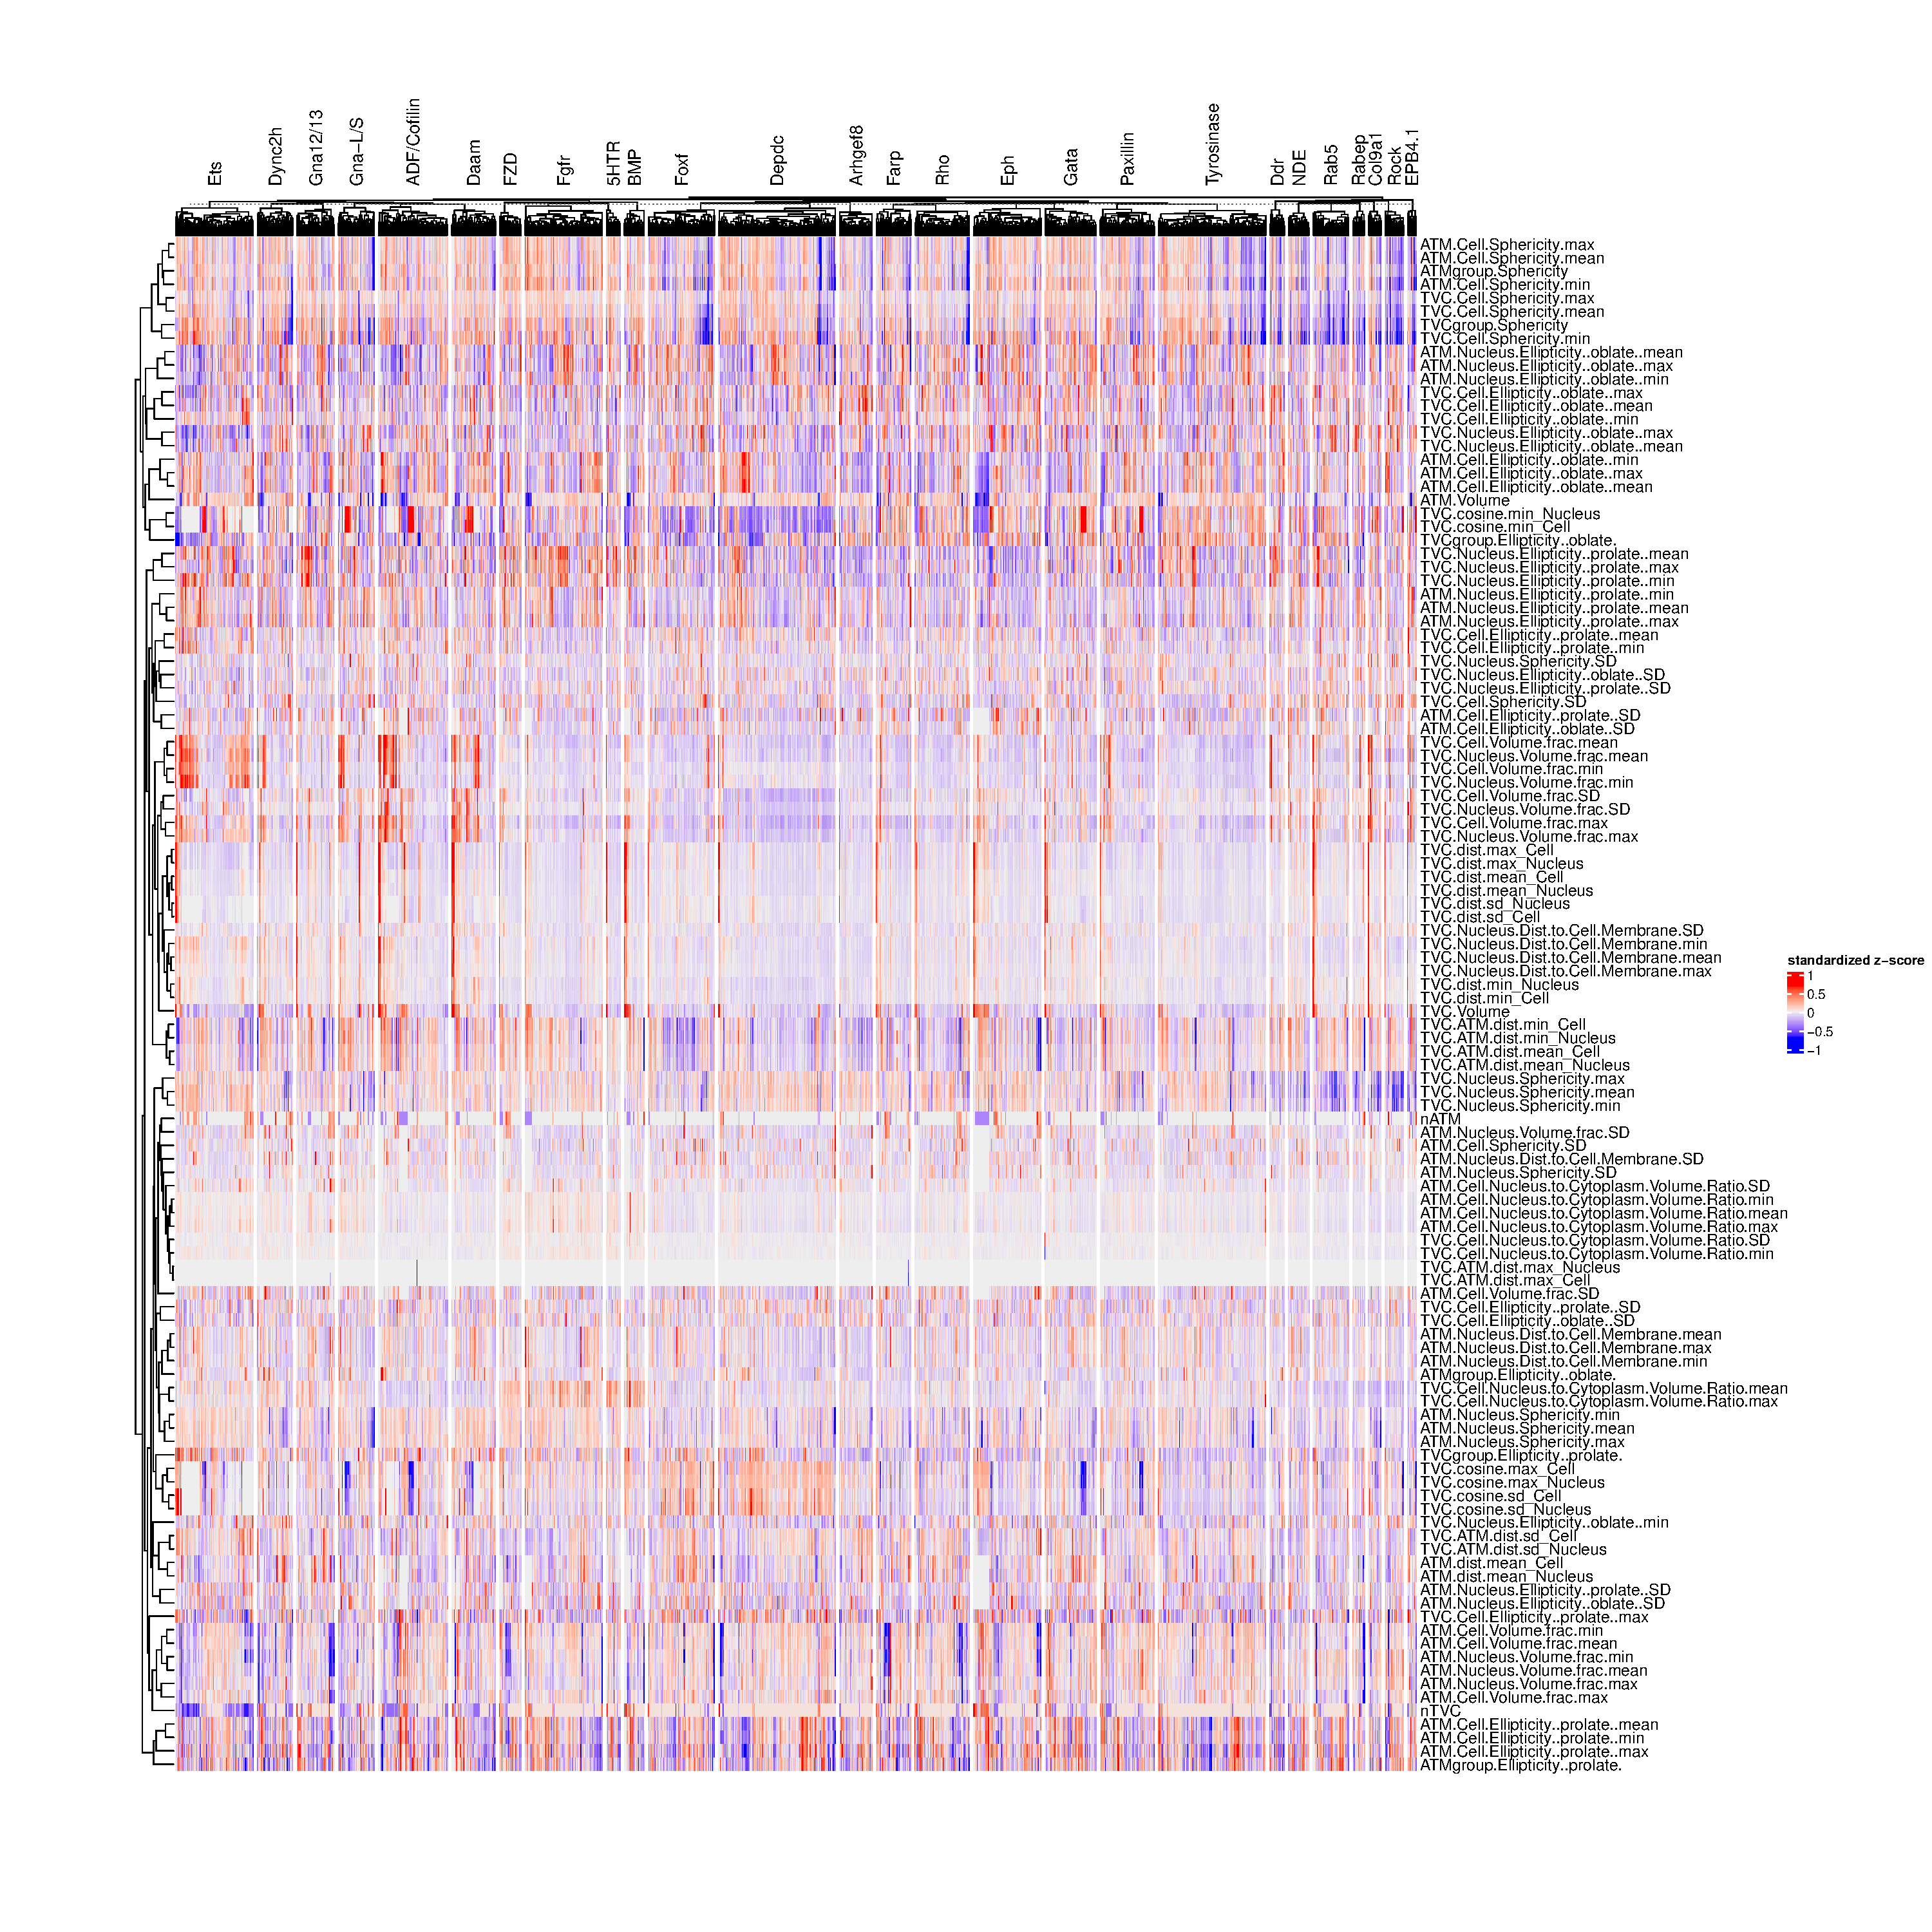
\includegraphics[width=\textwidth]{params.pdf}
		\end{column}
	\end{columns}
}

\frame{
	\frametitle{}
	\begin{columns}
		\begin{column}{0.50\textwidth}
			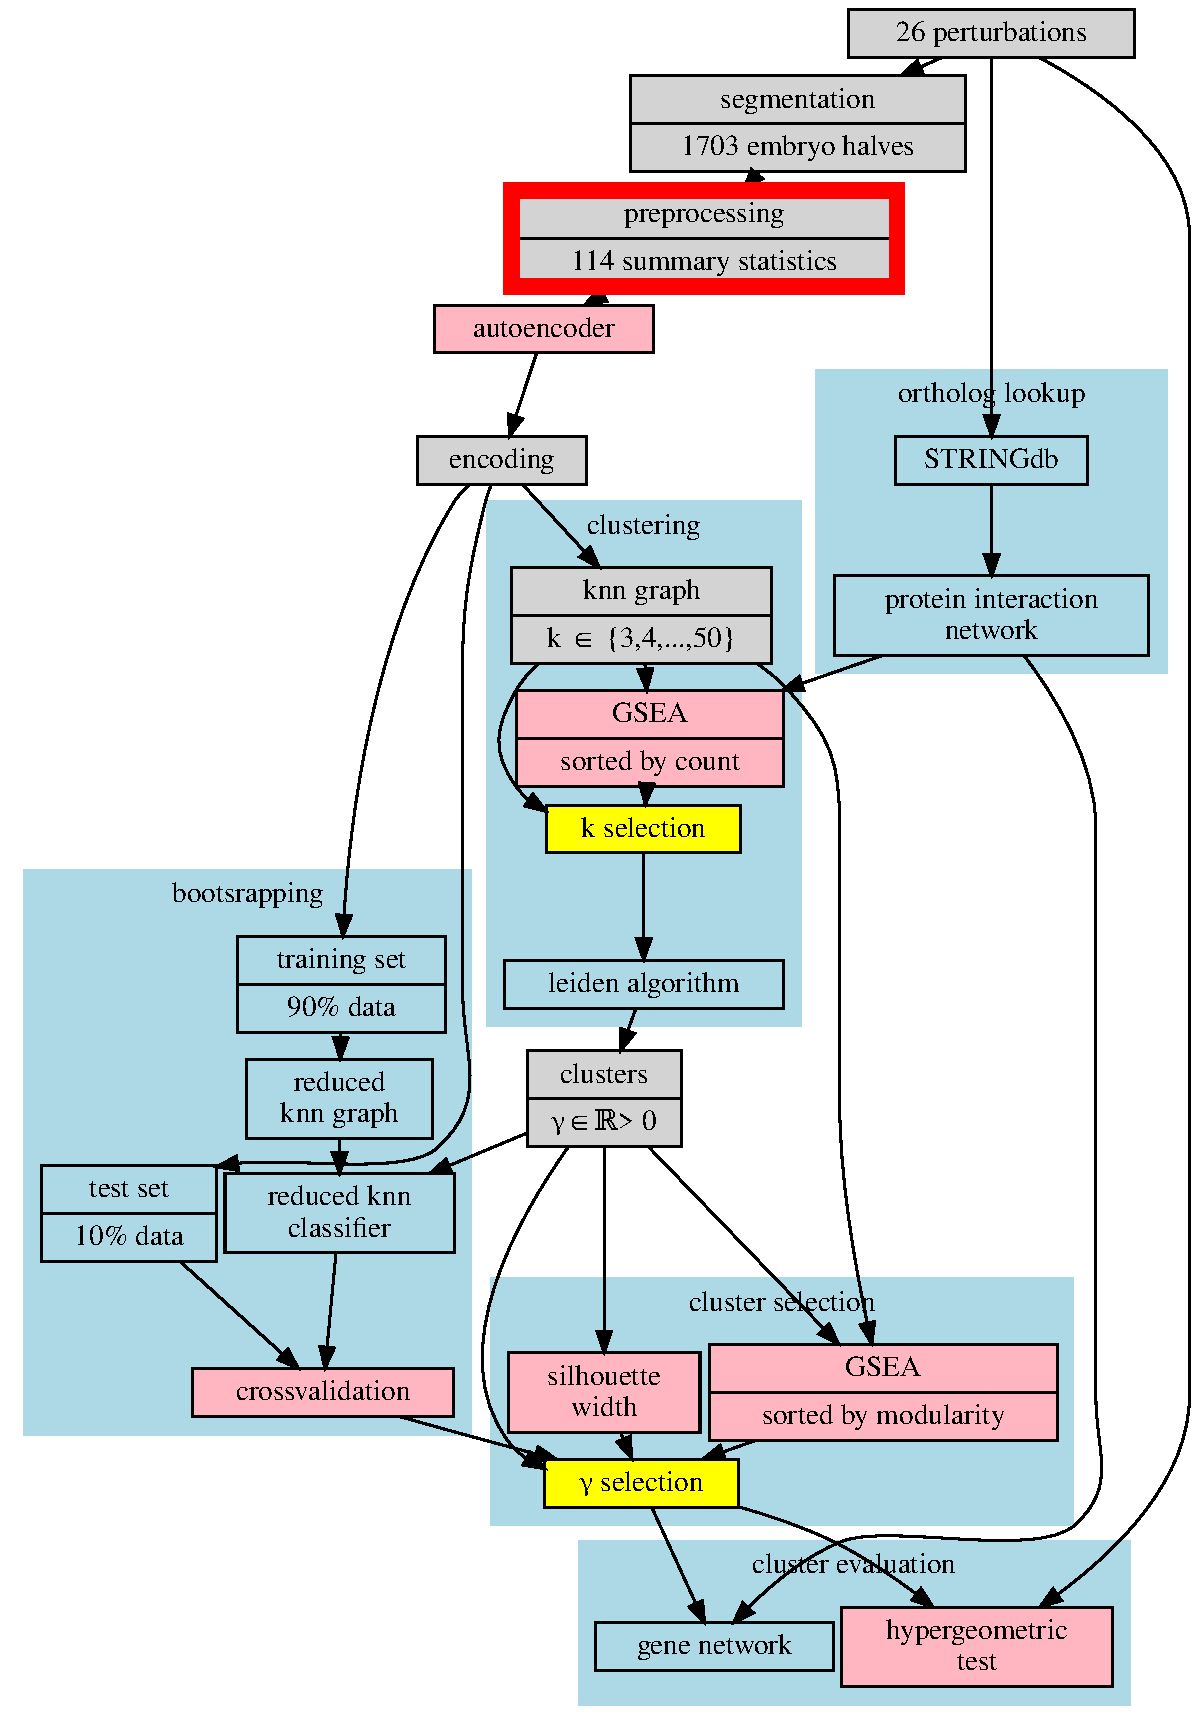
\includegraphics[width=\textwidth]{flowchart/preprocessing.pdf}
		\end{column}
		\begin{column}{0.50\textwidth}
			Many parameters are strongly correlated. This is undesirable because each parameter additively contributes to distance used for clustering, resulting in disproportionate weight being given to phenotypes captured by multiple parameters.
		\end{column}
	\end{columns}
}

\frame{
	\frametitle{}
	\begin{columns}
		\begin{column}{0.40\textwidth}
			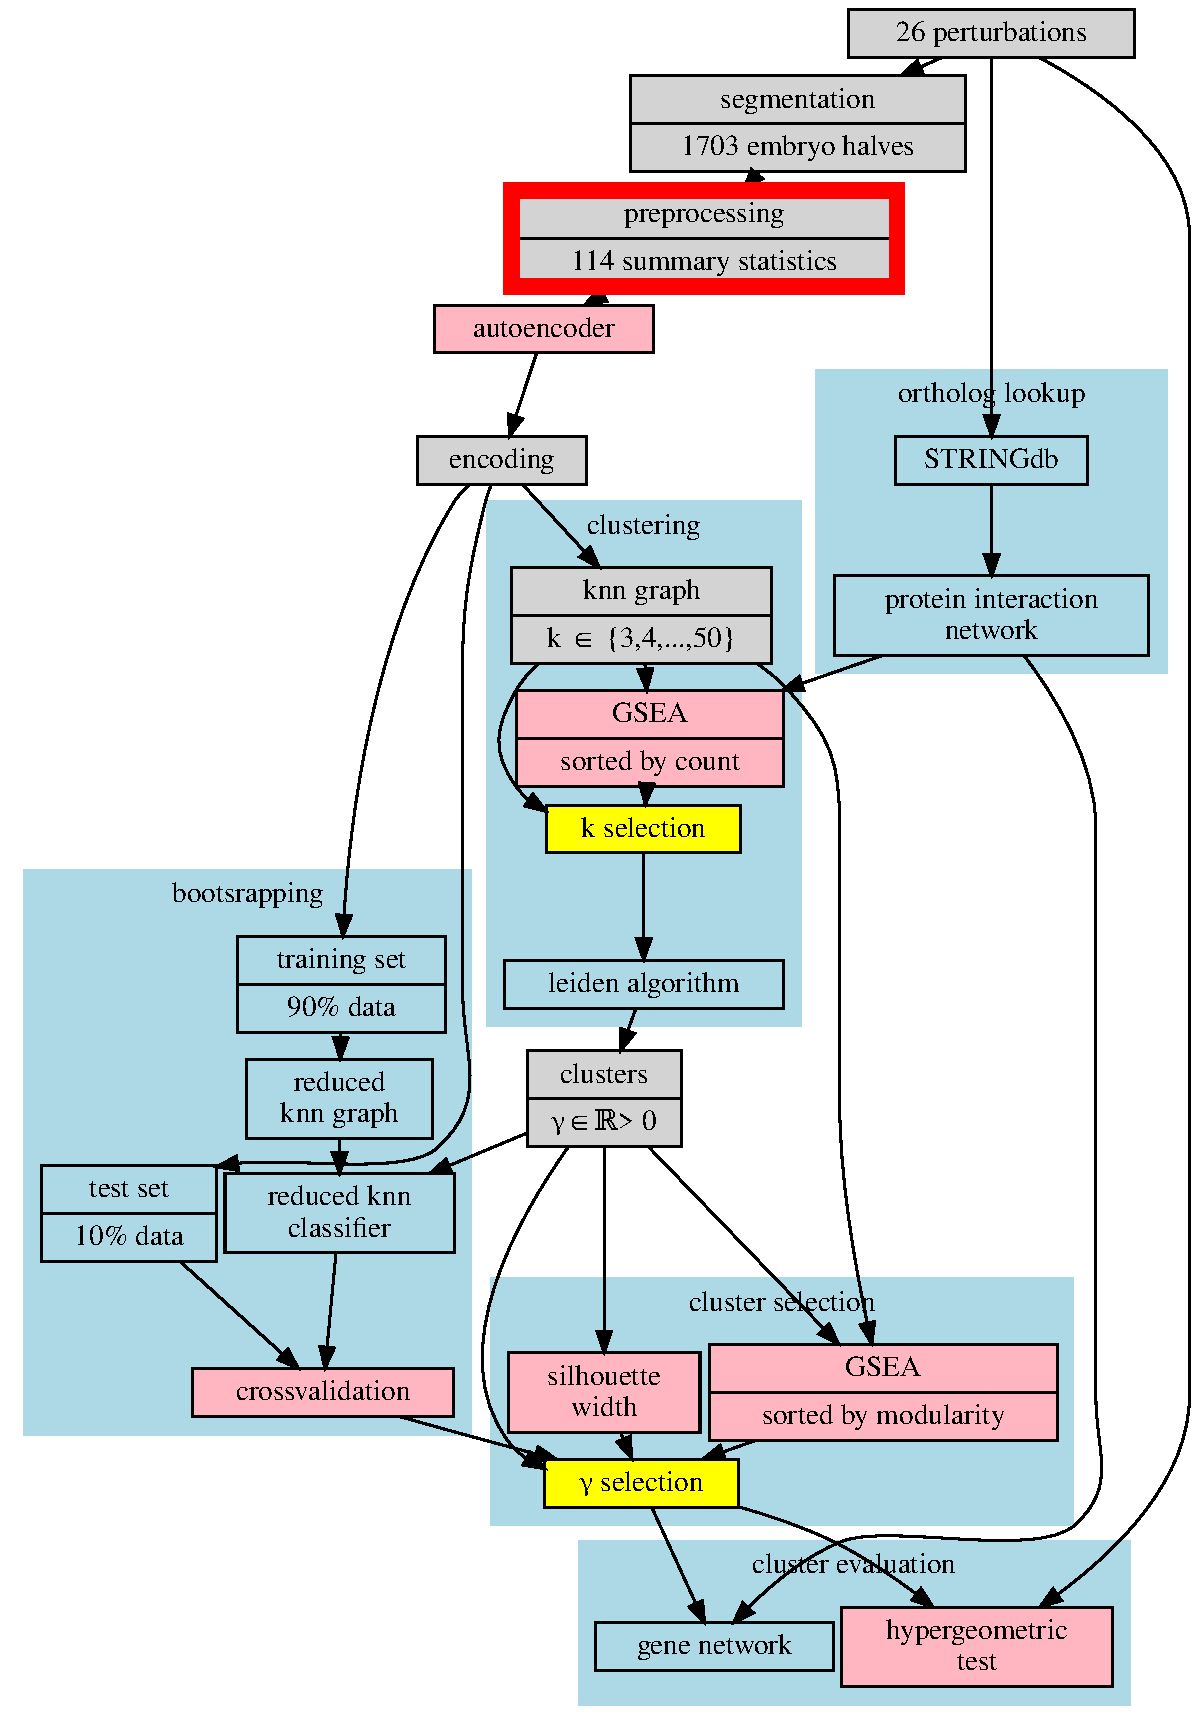
\includegraphics[width=\textwidth]{flowchart/preprocessing.pdf}
		\end{column}
		\begin{column}{0.80\textwidth}
			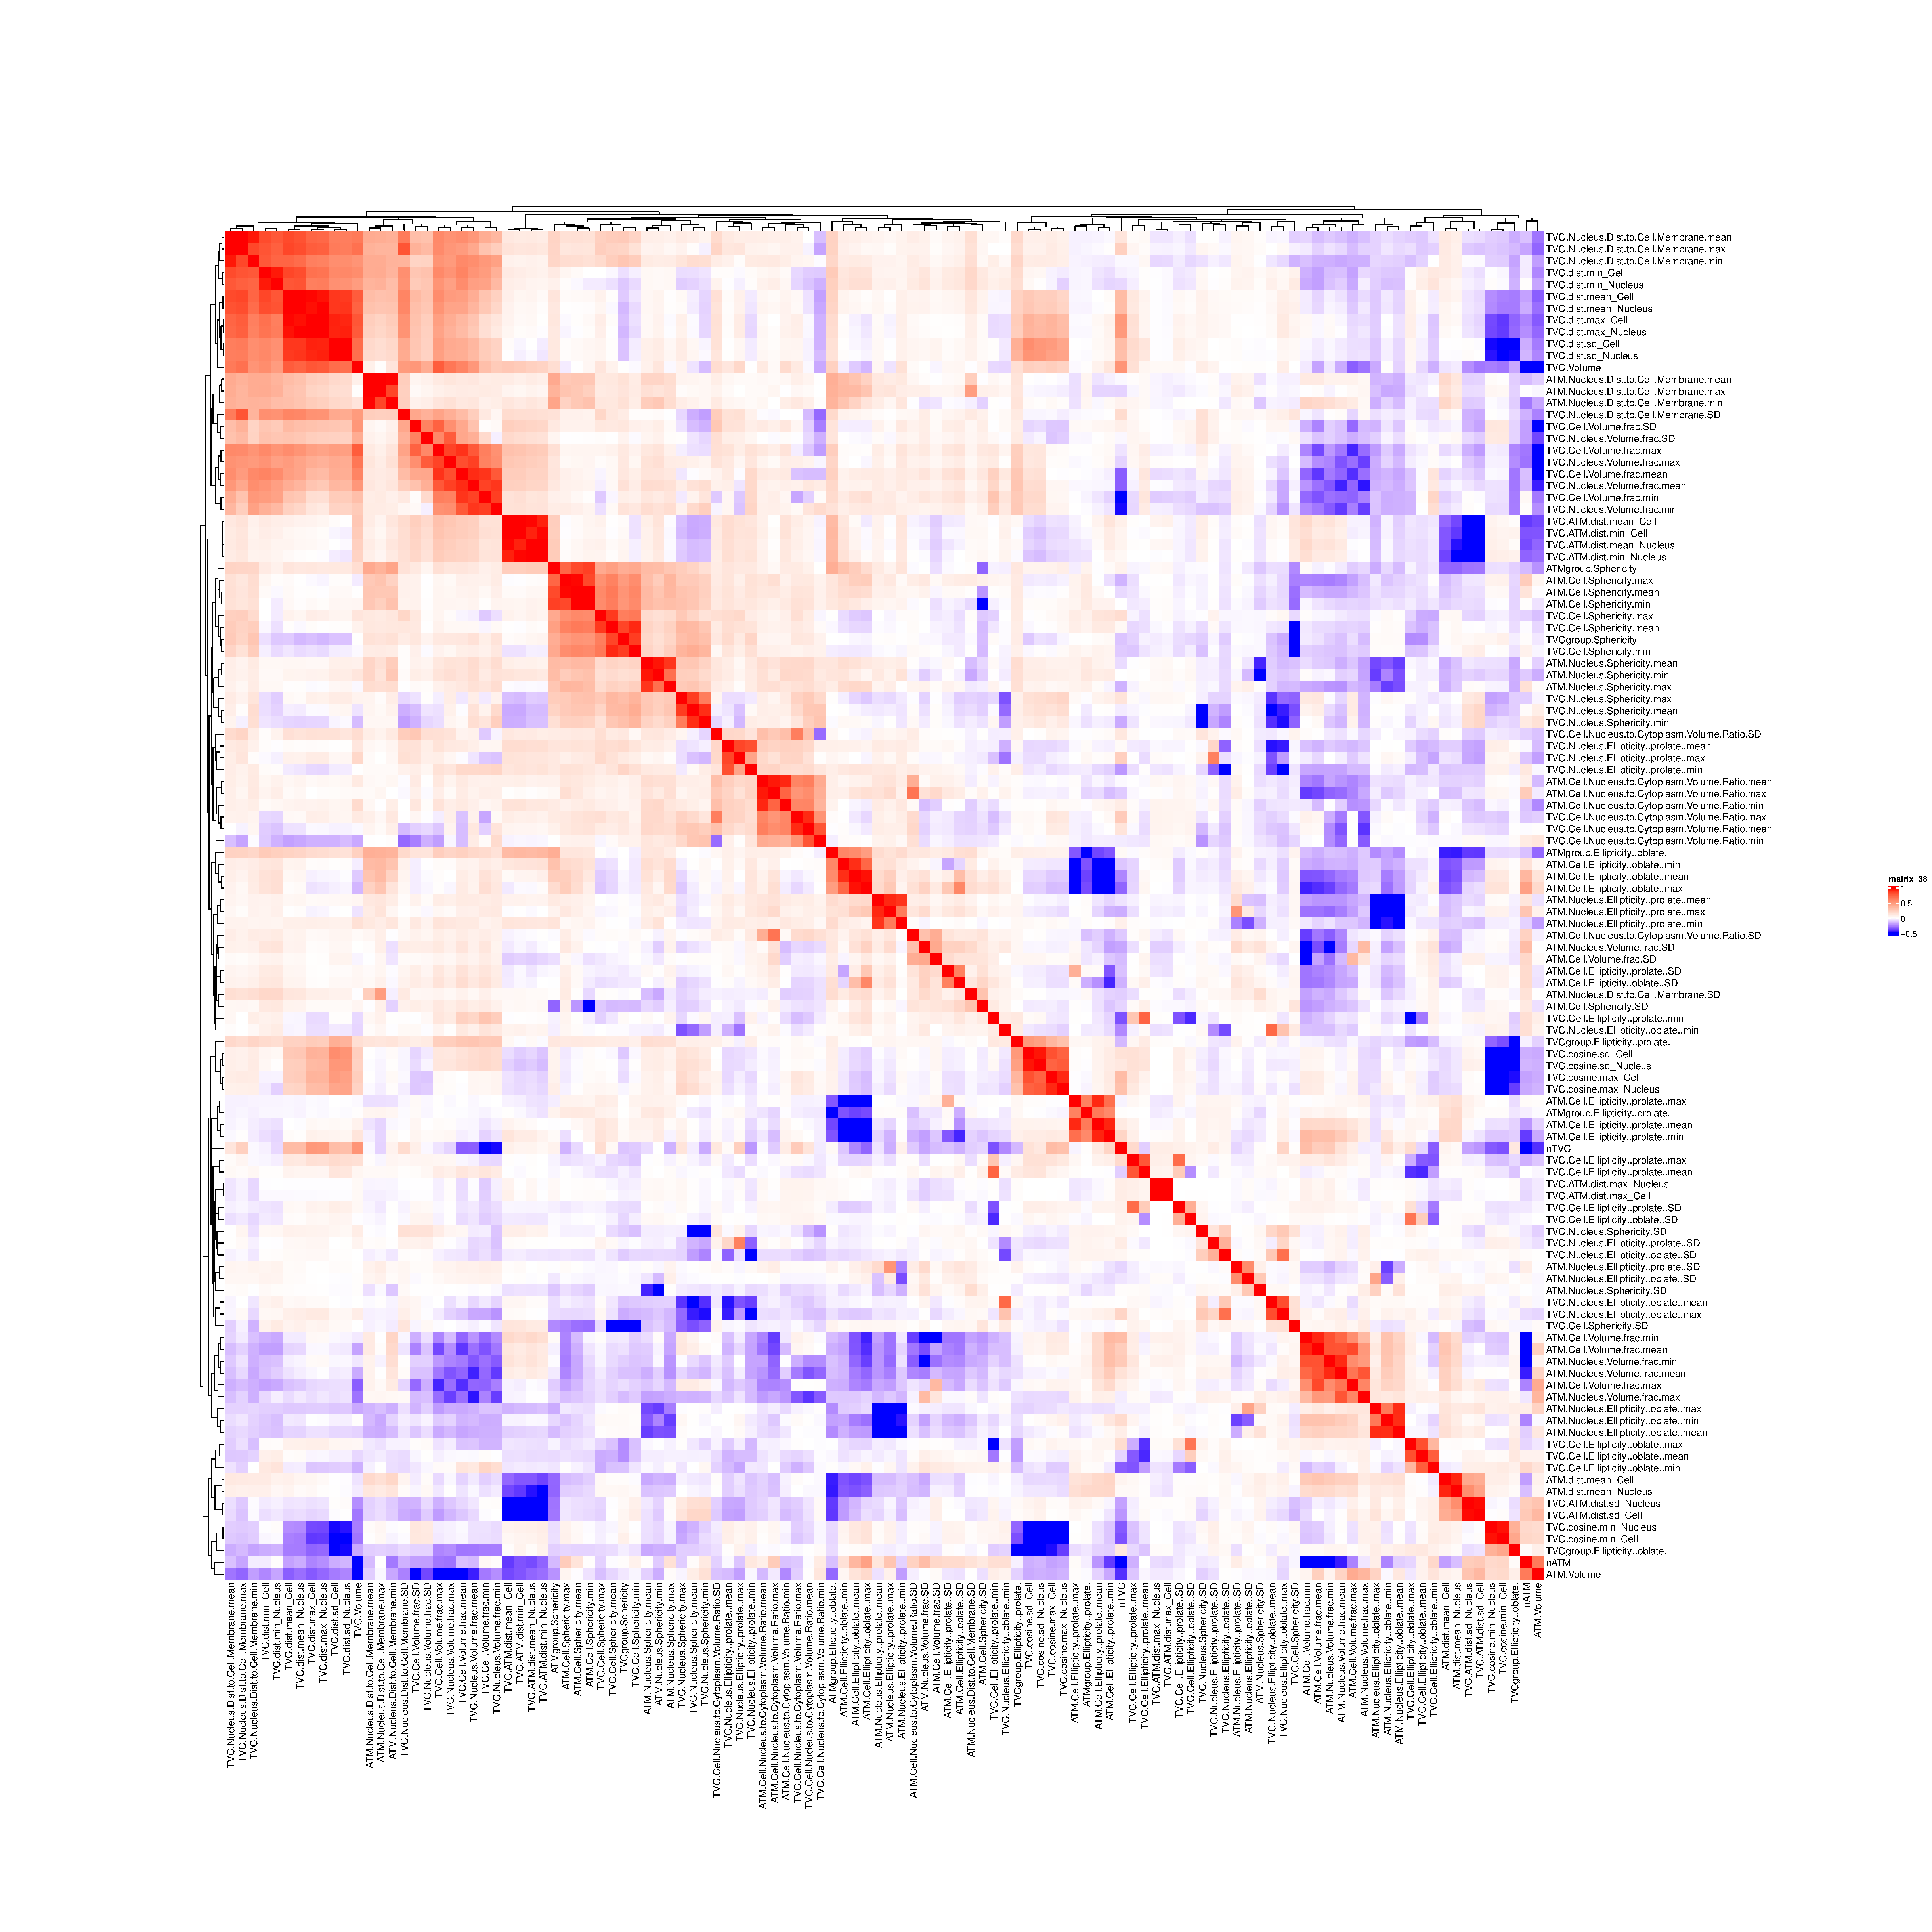
\includegraphics[width=\textwidth]{correlation.pdf}
		\end{column}
	\end{columns}
}

\frame{
	\frametitle{}
	\begin{columns}
		\begin{column}{0.50\textwidth}
			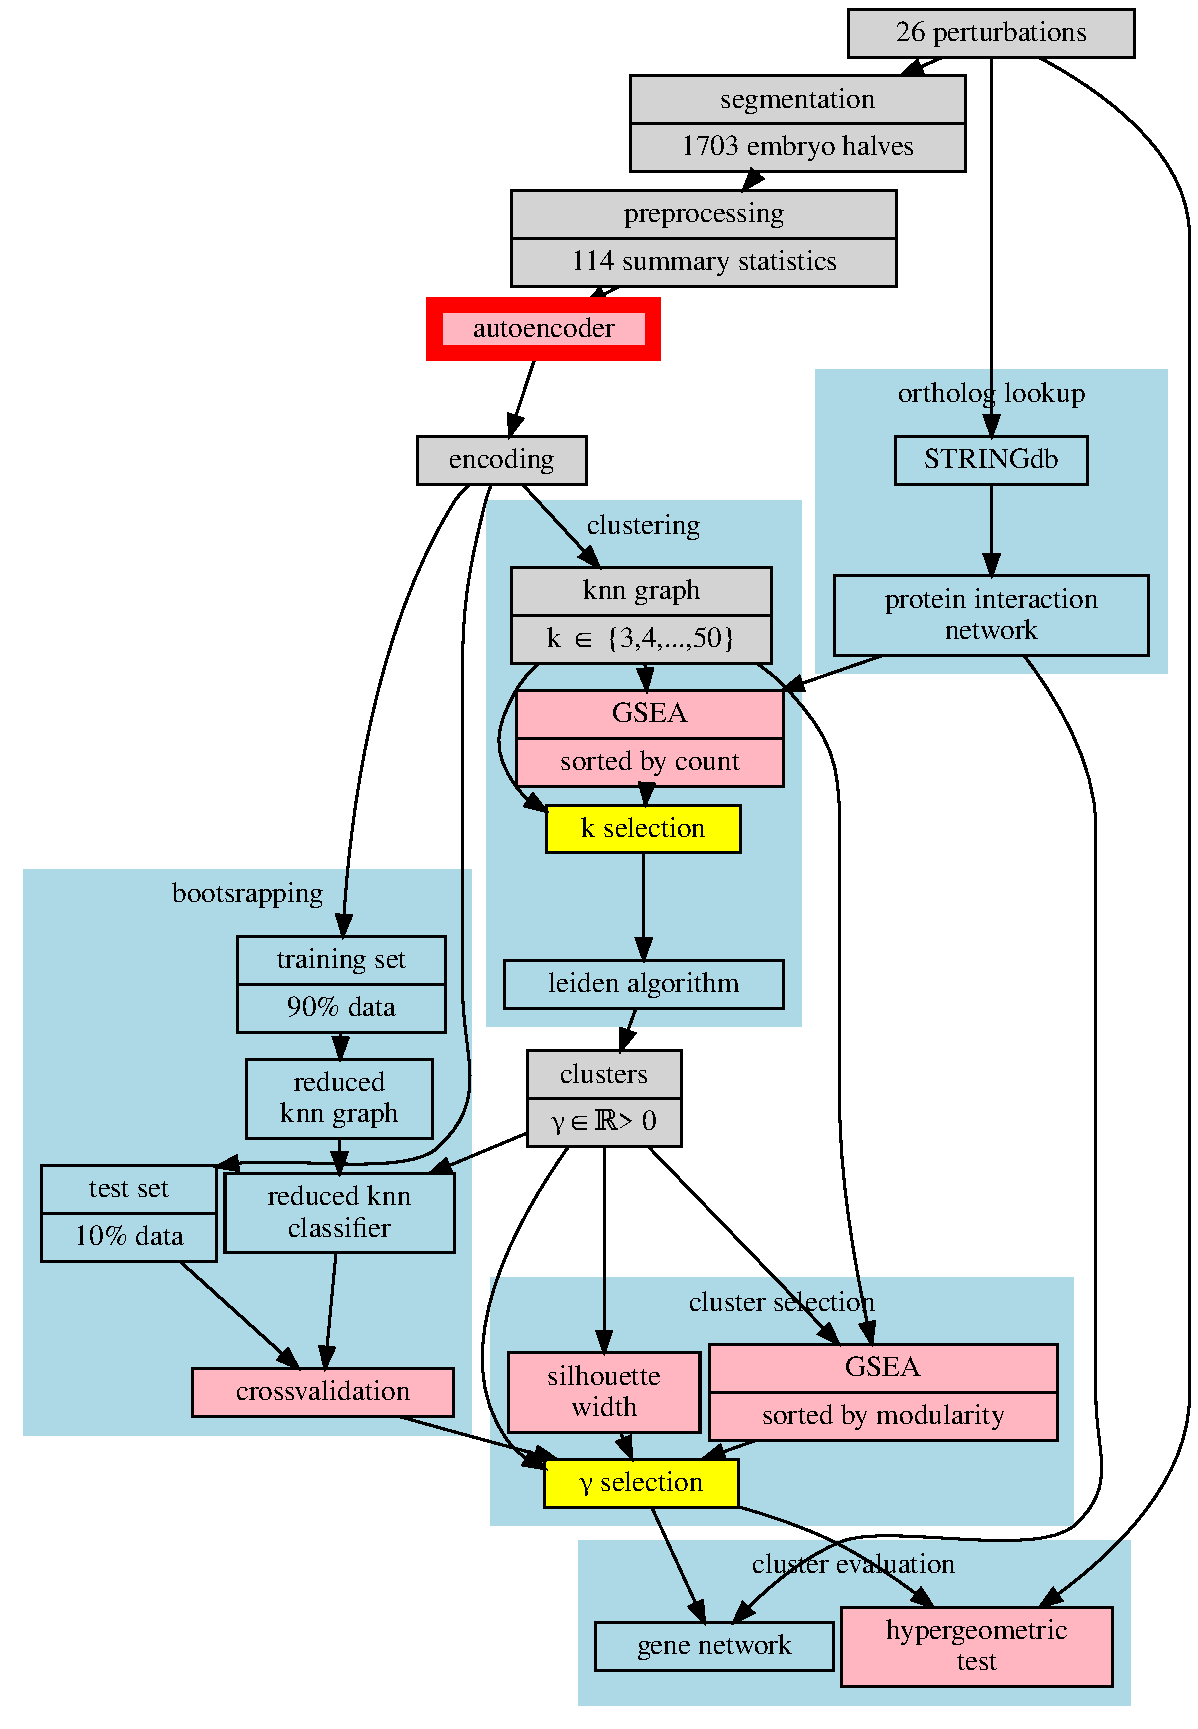
\includegraphics[width=\textwidth]{flowchart/autoencoder.pdf}
		\end{column}
		\begin{column}{0.50\textwidth}
			An autoencoder is a method of dimension reduction that uses a neural network to find a lower dimensional encoding which can be decoded to recover the input. This reduces exaggeration of distance due to the number of parameters measured.
		\end{column}
	\end{columns}
}


\frame{
	\frametitle{}
	\begin{columns}
		\begin{column}{0.50\textwidth}
			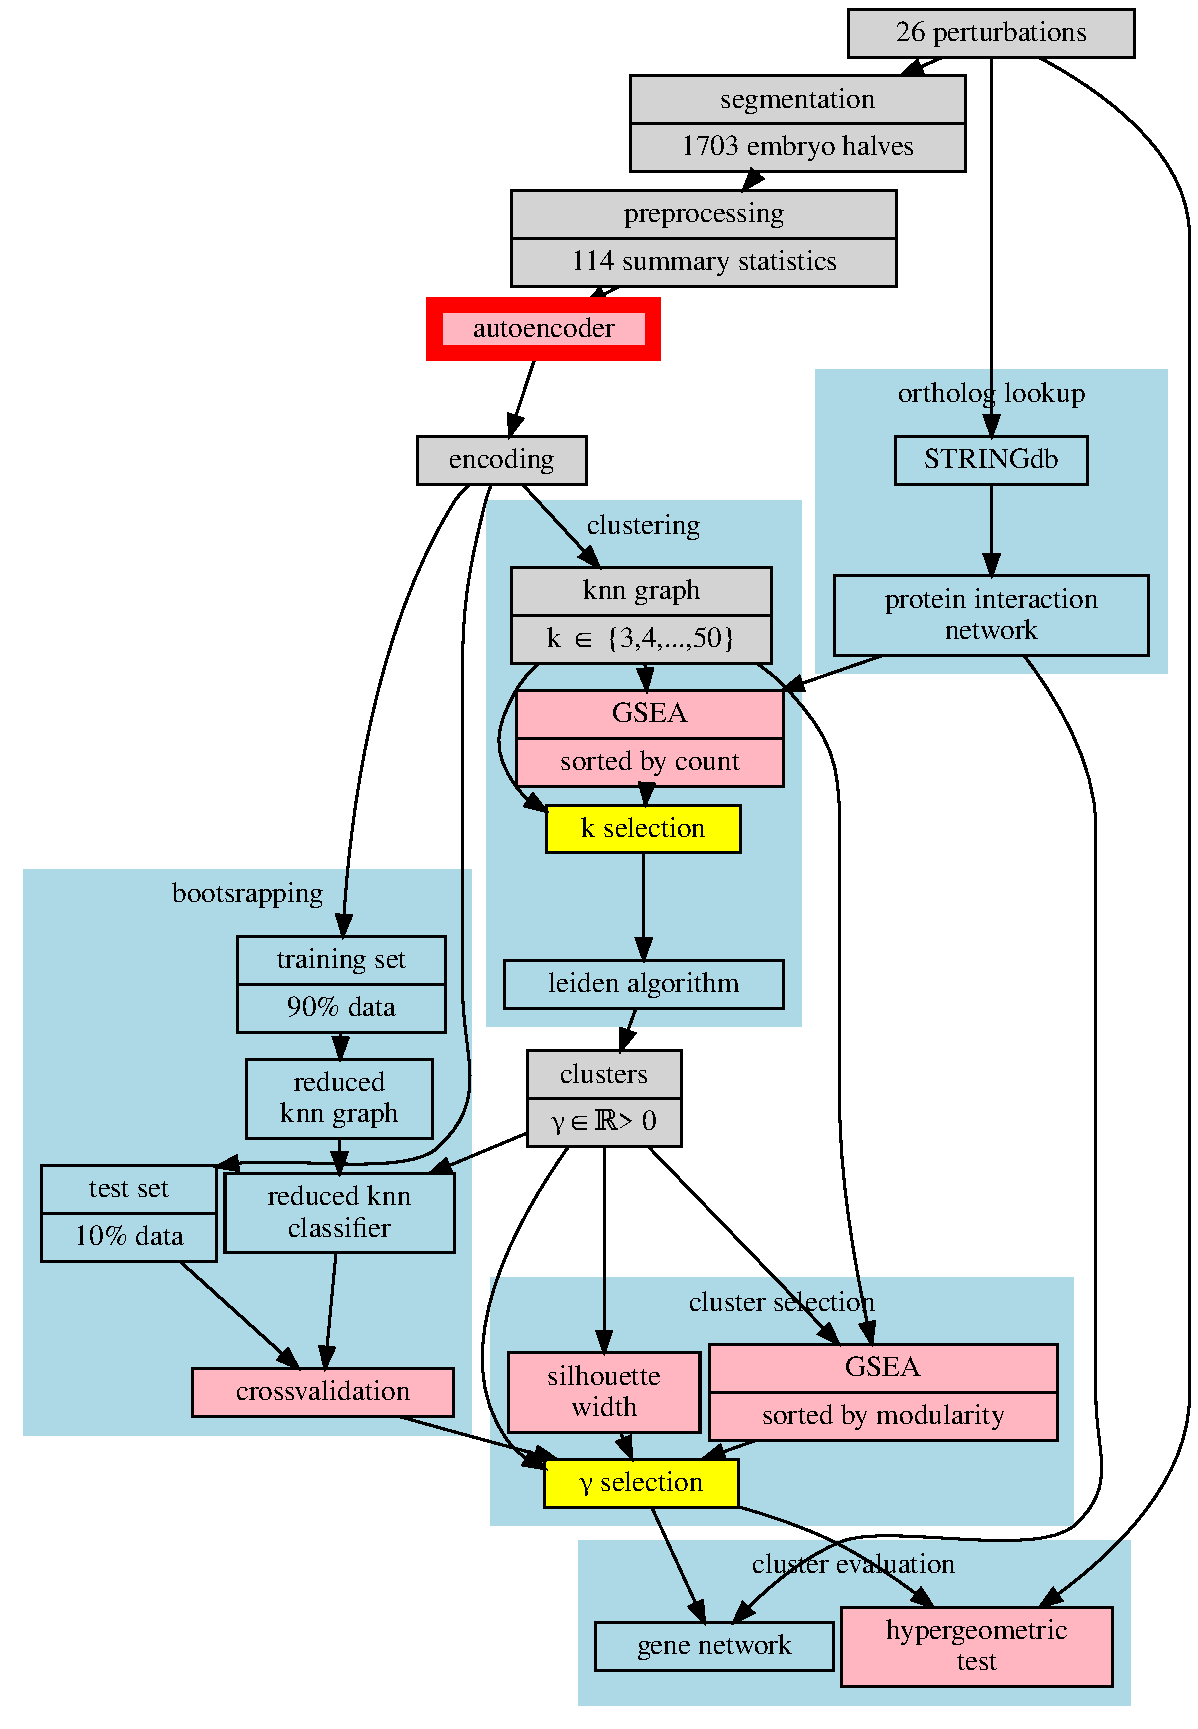
\includegraphics[width=\textwidth]{flowchart/autoencoder.pdf}
		\end{column}
		\begin{column}{0.50\textwidth}
			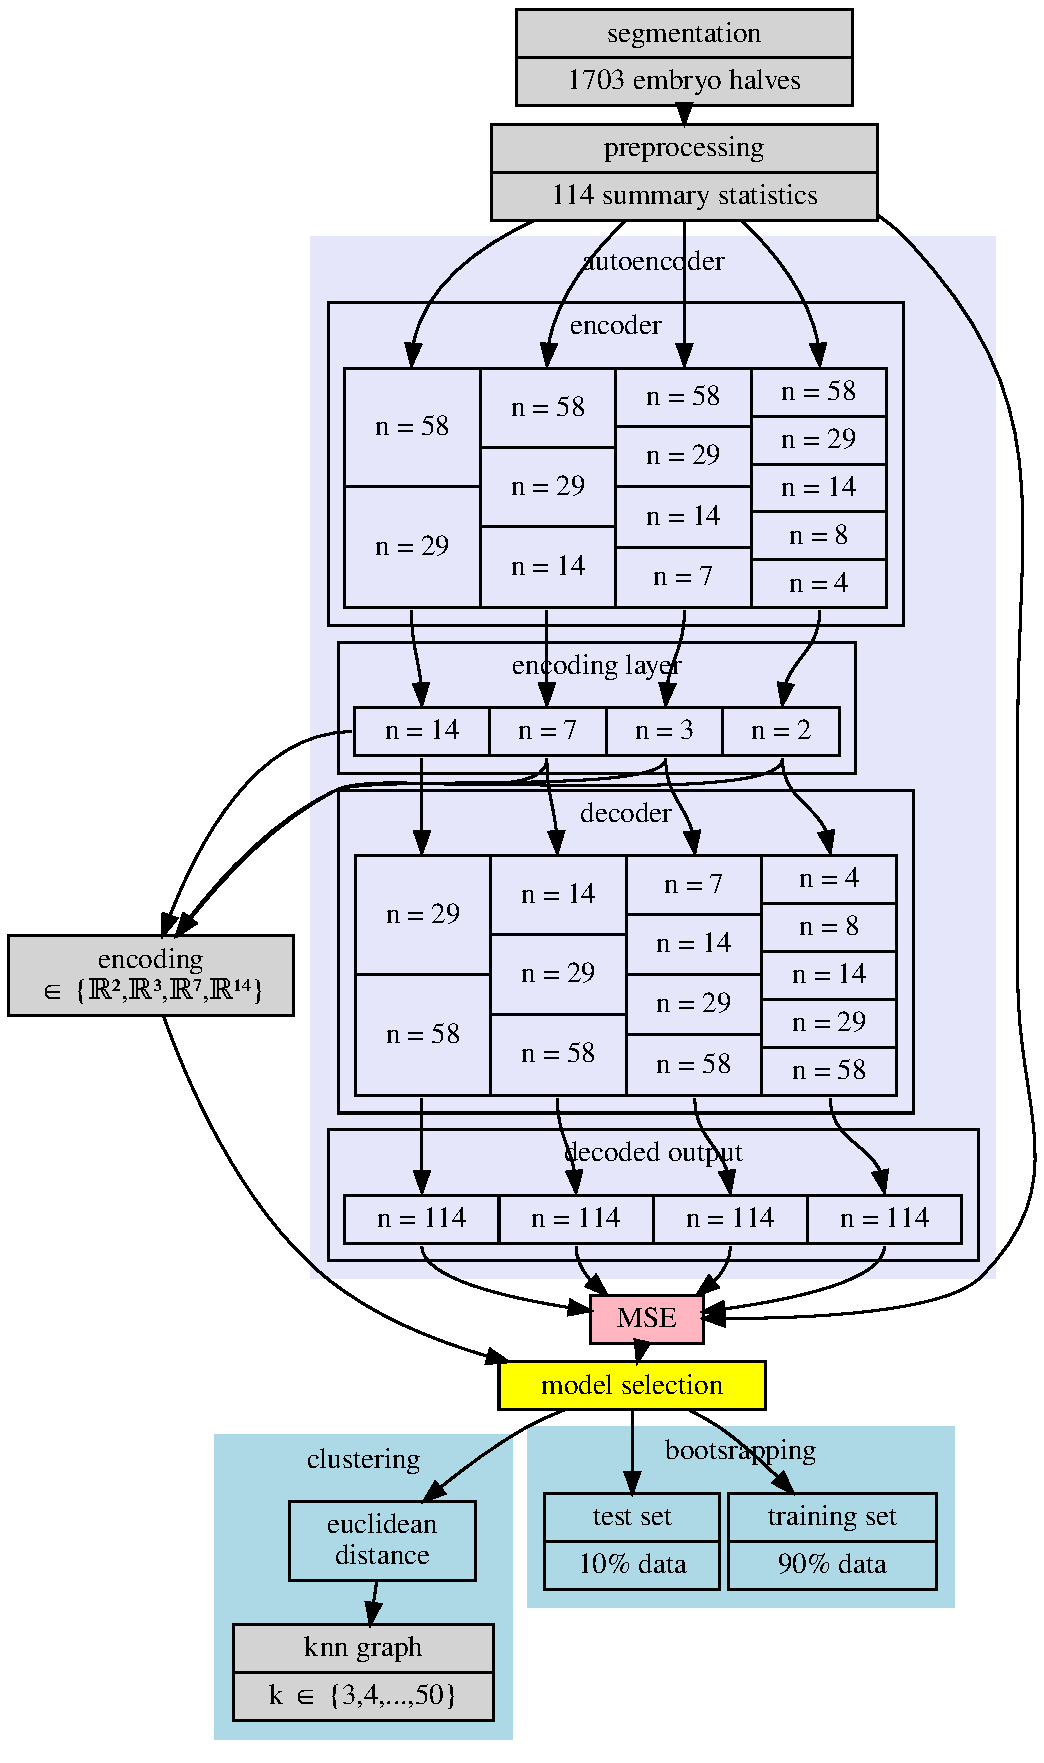
\includegraphics[width=\textwidth]{flowchart/autoencoder.dot.pdf}
		\end{column}
	\end{columns}
}

\frame{
	\frametitle{}
	\begin{columns}
		\begin{column}{0.50\textwidth}
			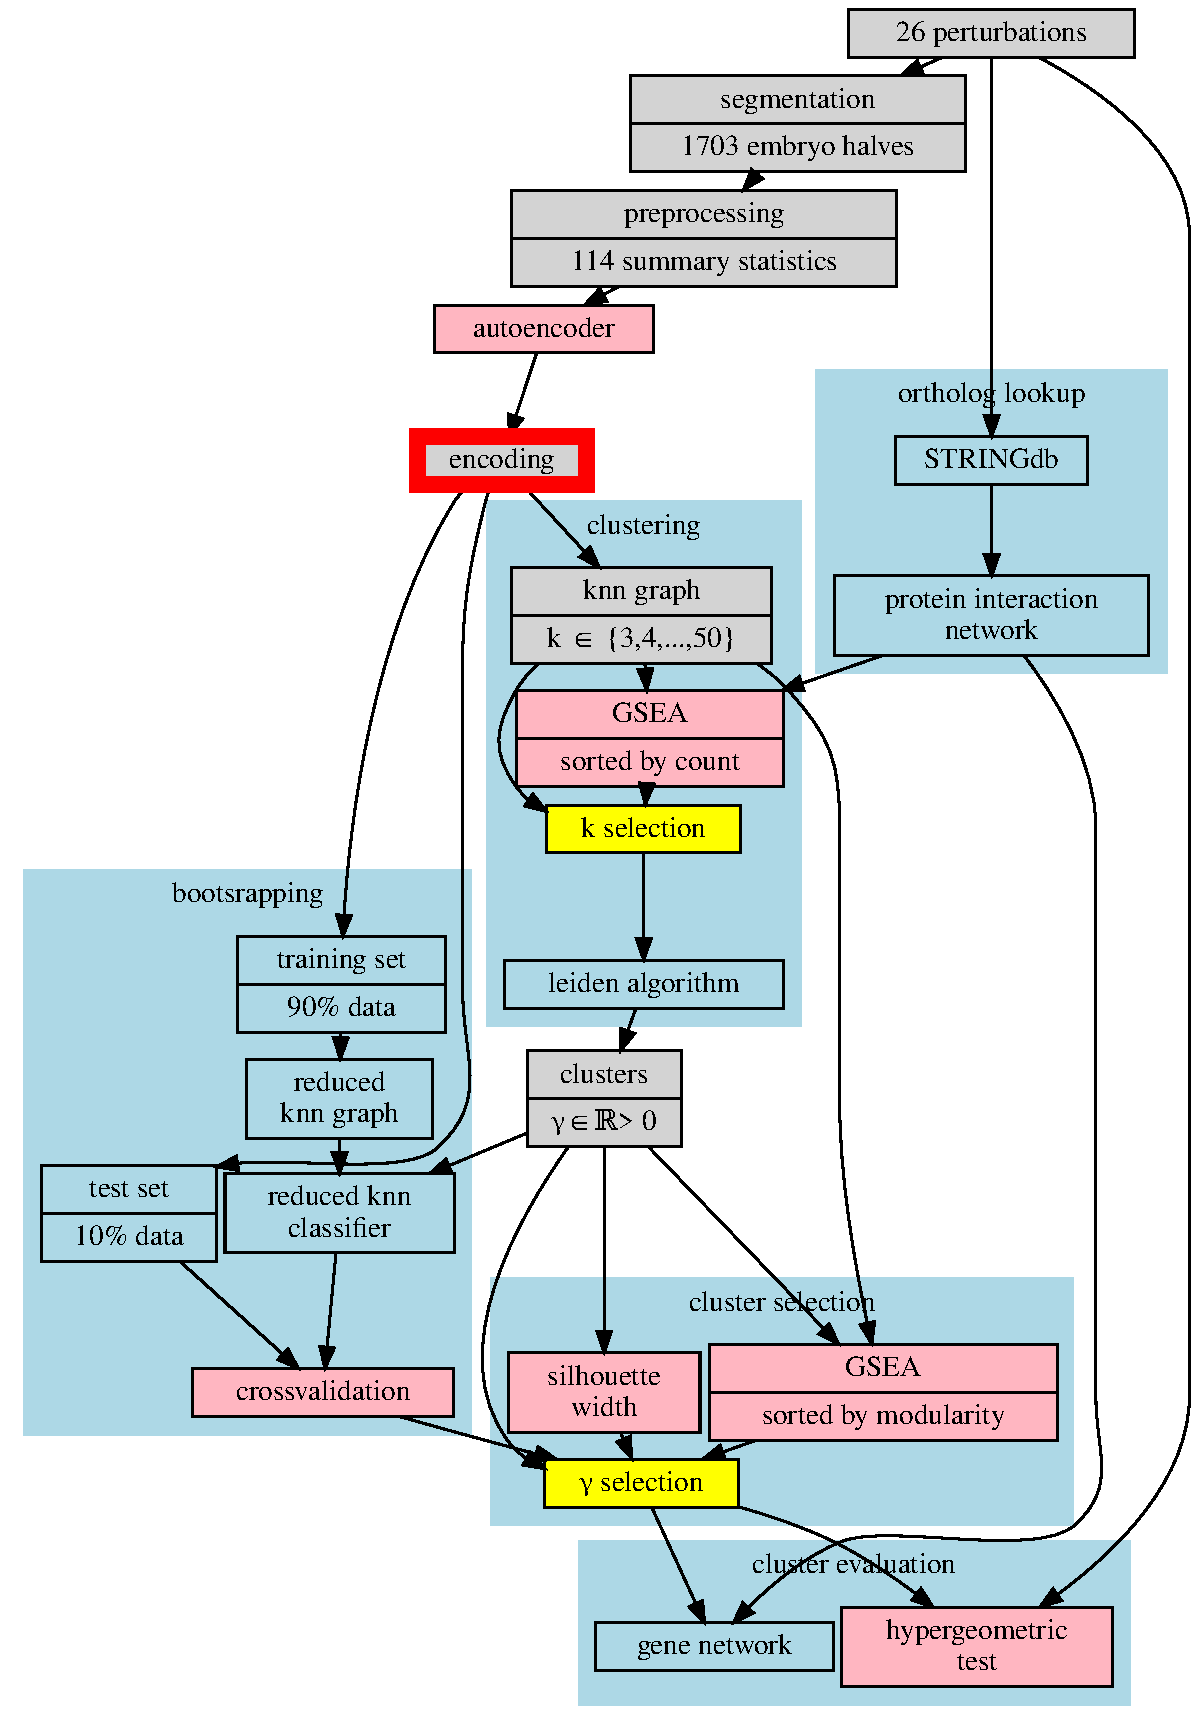
\includegraphics[width=\textwidth]{flowchart/encoding.pdf}
		\end{column}
		\begin{column}{0.50\textwidth}
			More than 2D produced only marginal improvement.
		\end{column}
	\end{columns}
}

\frame{
	\frametitle{}
	\begin{columns}
		\begin{column}{0.40\textwidth}
			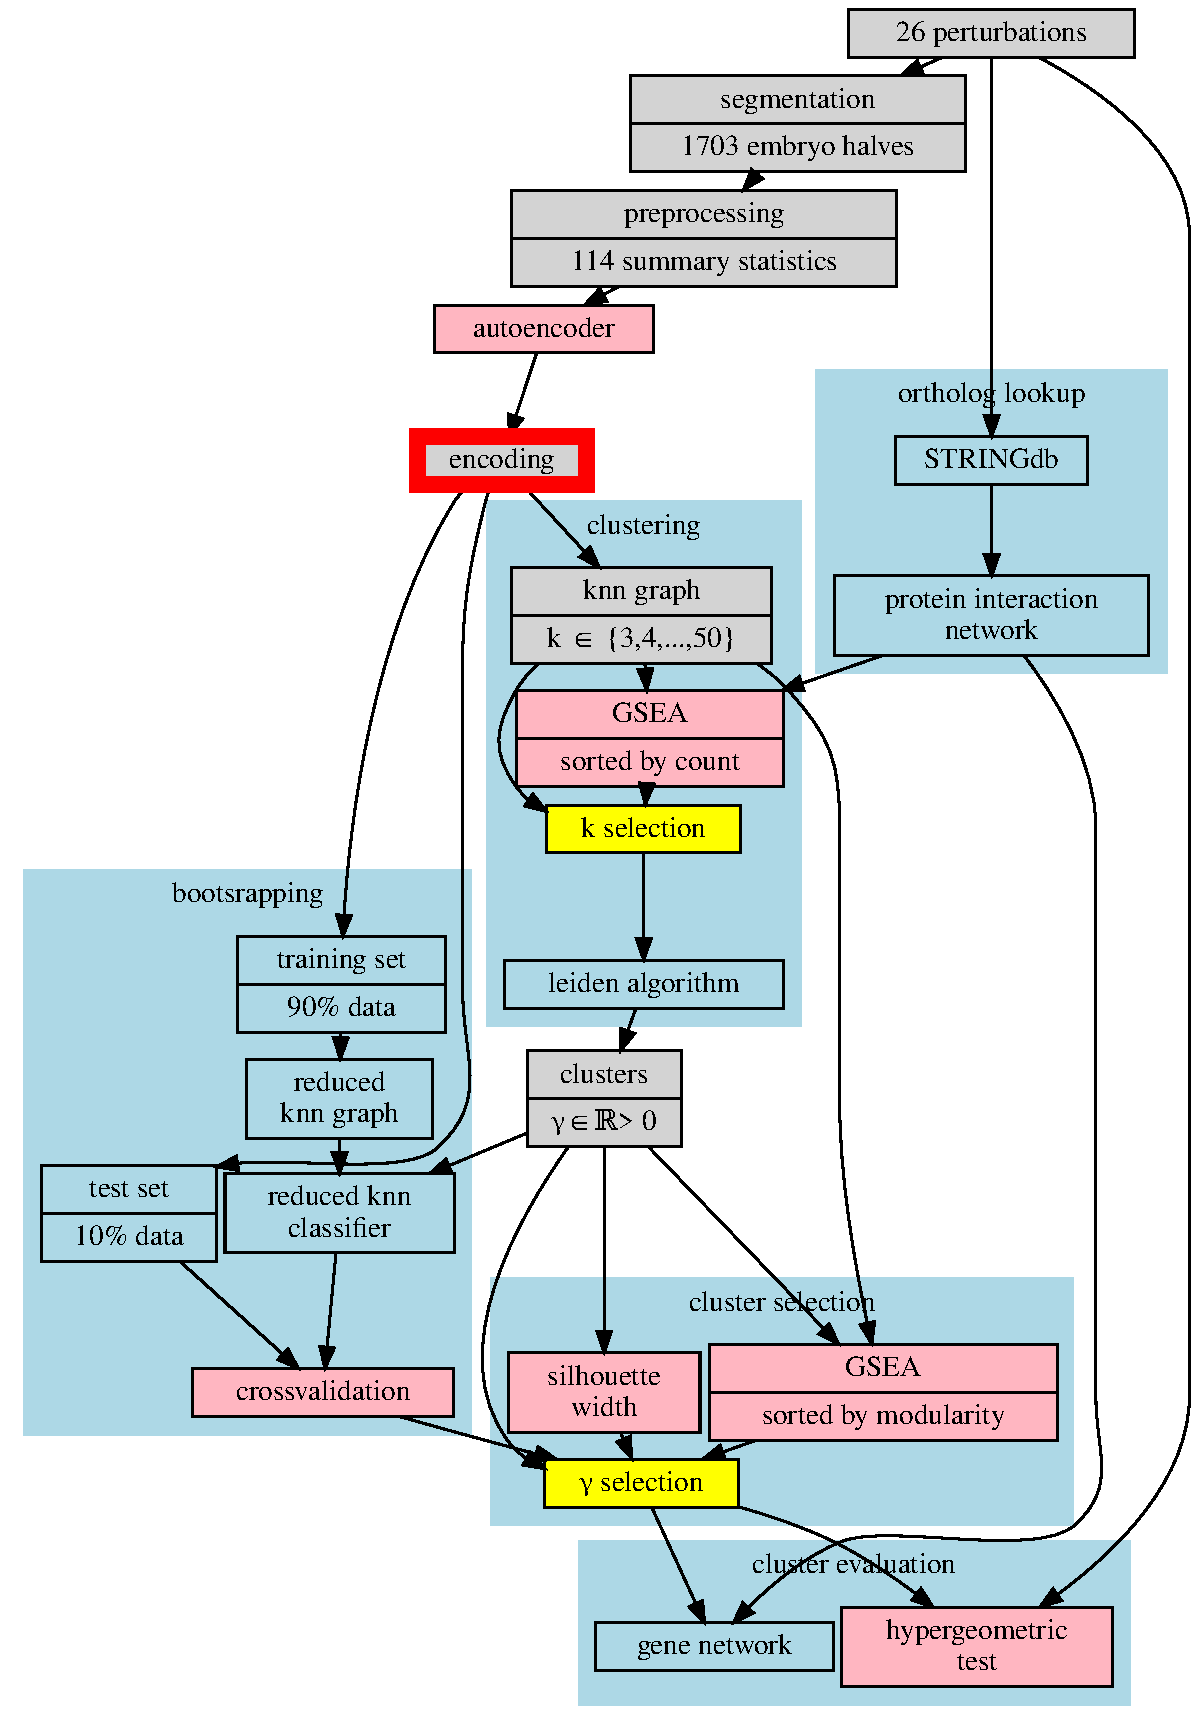
\includegraphics[width=\textwidth]{flowchart/encoding.pdf}
		\end{column}
		\begin{column}{0.80\textwidth}
			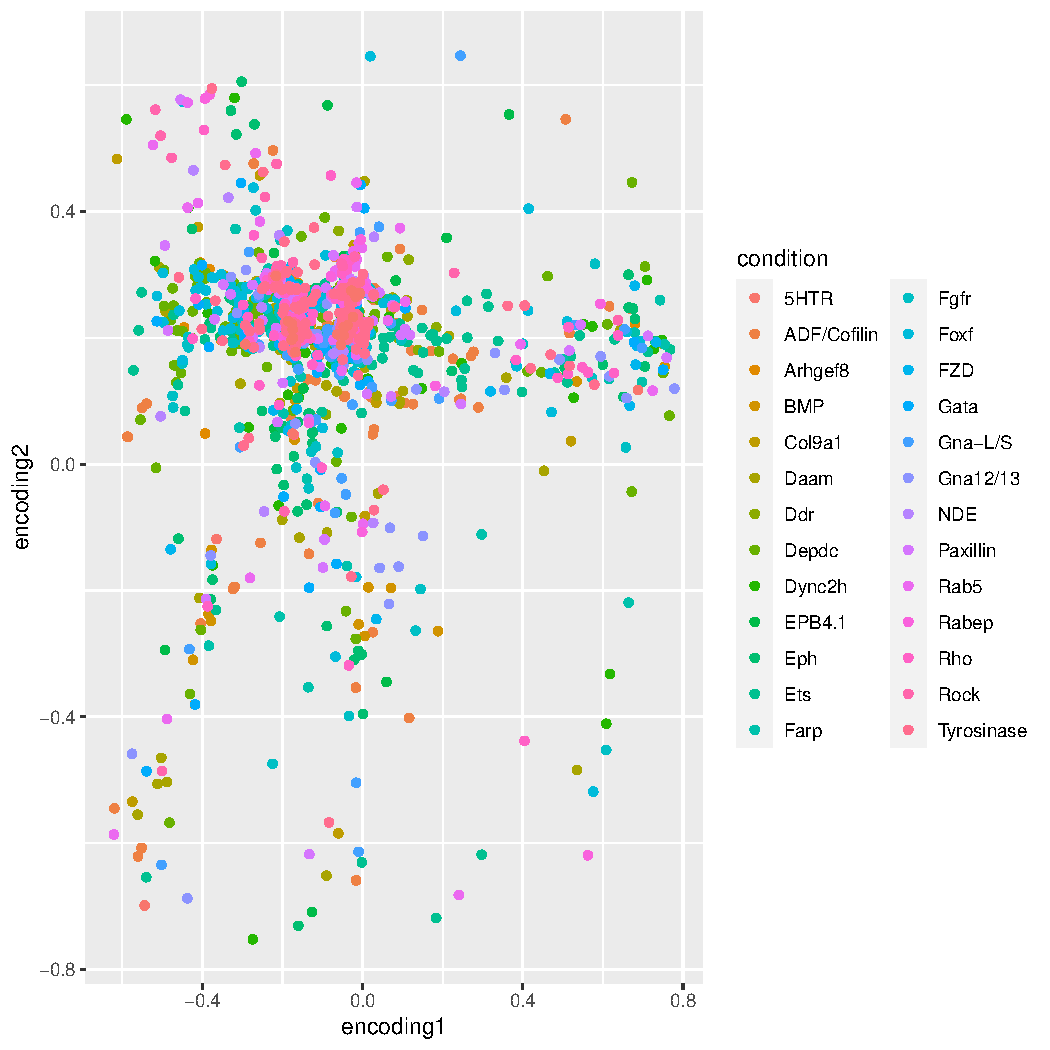
\includegraphics[width=\textwidth]{encoding.pdf}
		\end{column}
	\end{columns}
}

\frame{
	\frametitle{}
	\begin{columns}
		\begin{column}{0.50\textwidth}
			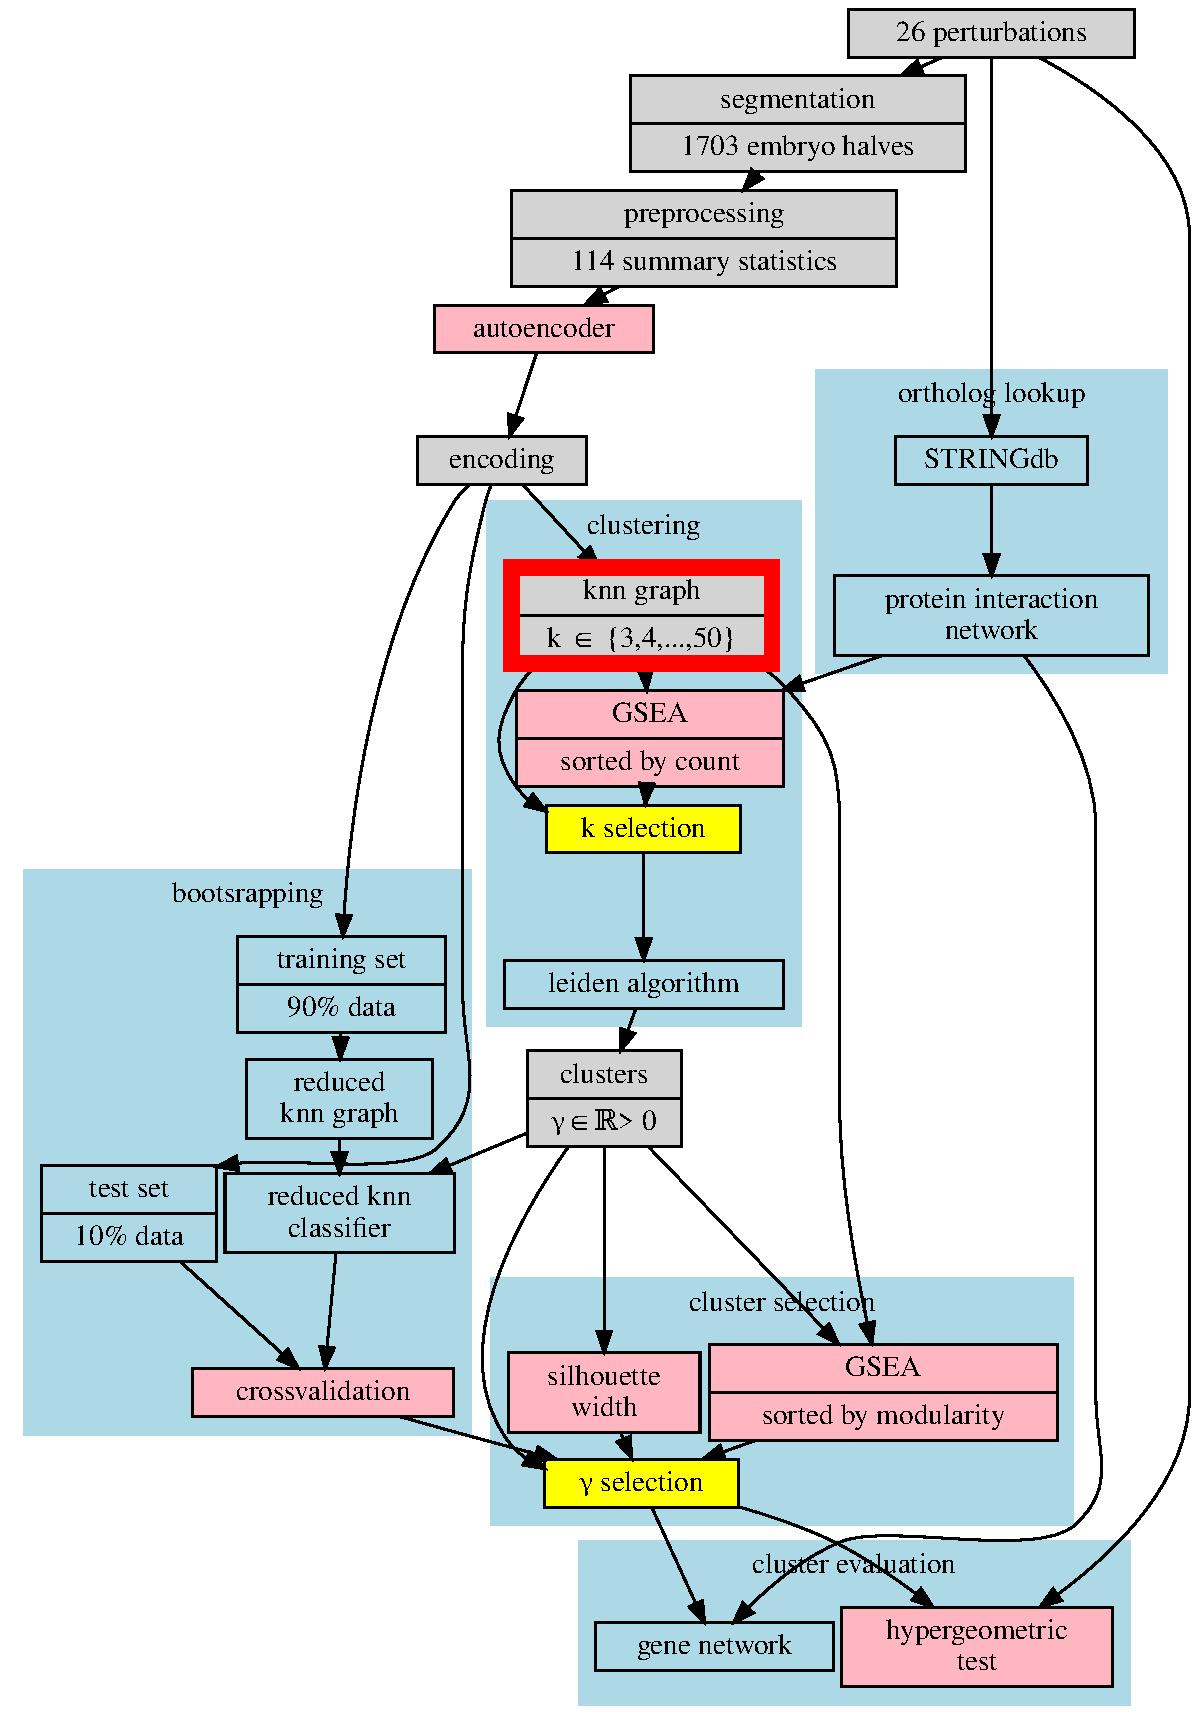
\includegraphics[width=\textwidth]{flowchart/knn.pdf}
		\end{column}
		\begin{column}{0.50\textwidth}
			A kNN graph is constructed from euclidean distance calculated from the encoding layer.
		\end{column}
	\end{columns}
}


\frame{
	\frametitle{}
	\begin{columns}
		\begin{column}{0.40\textwidth}
			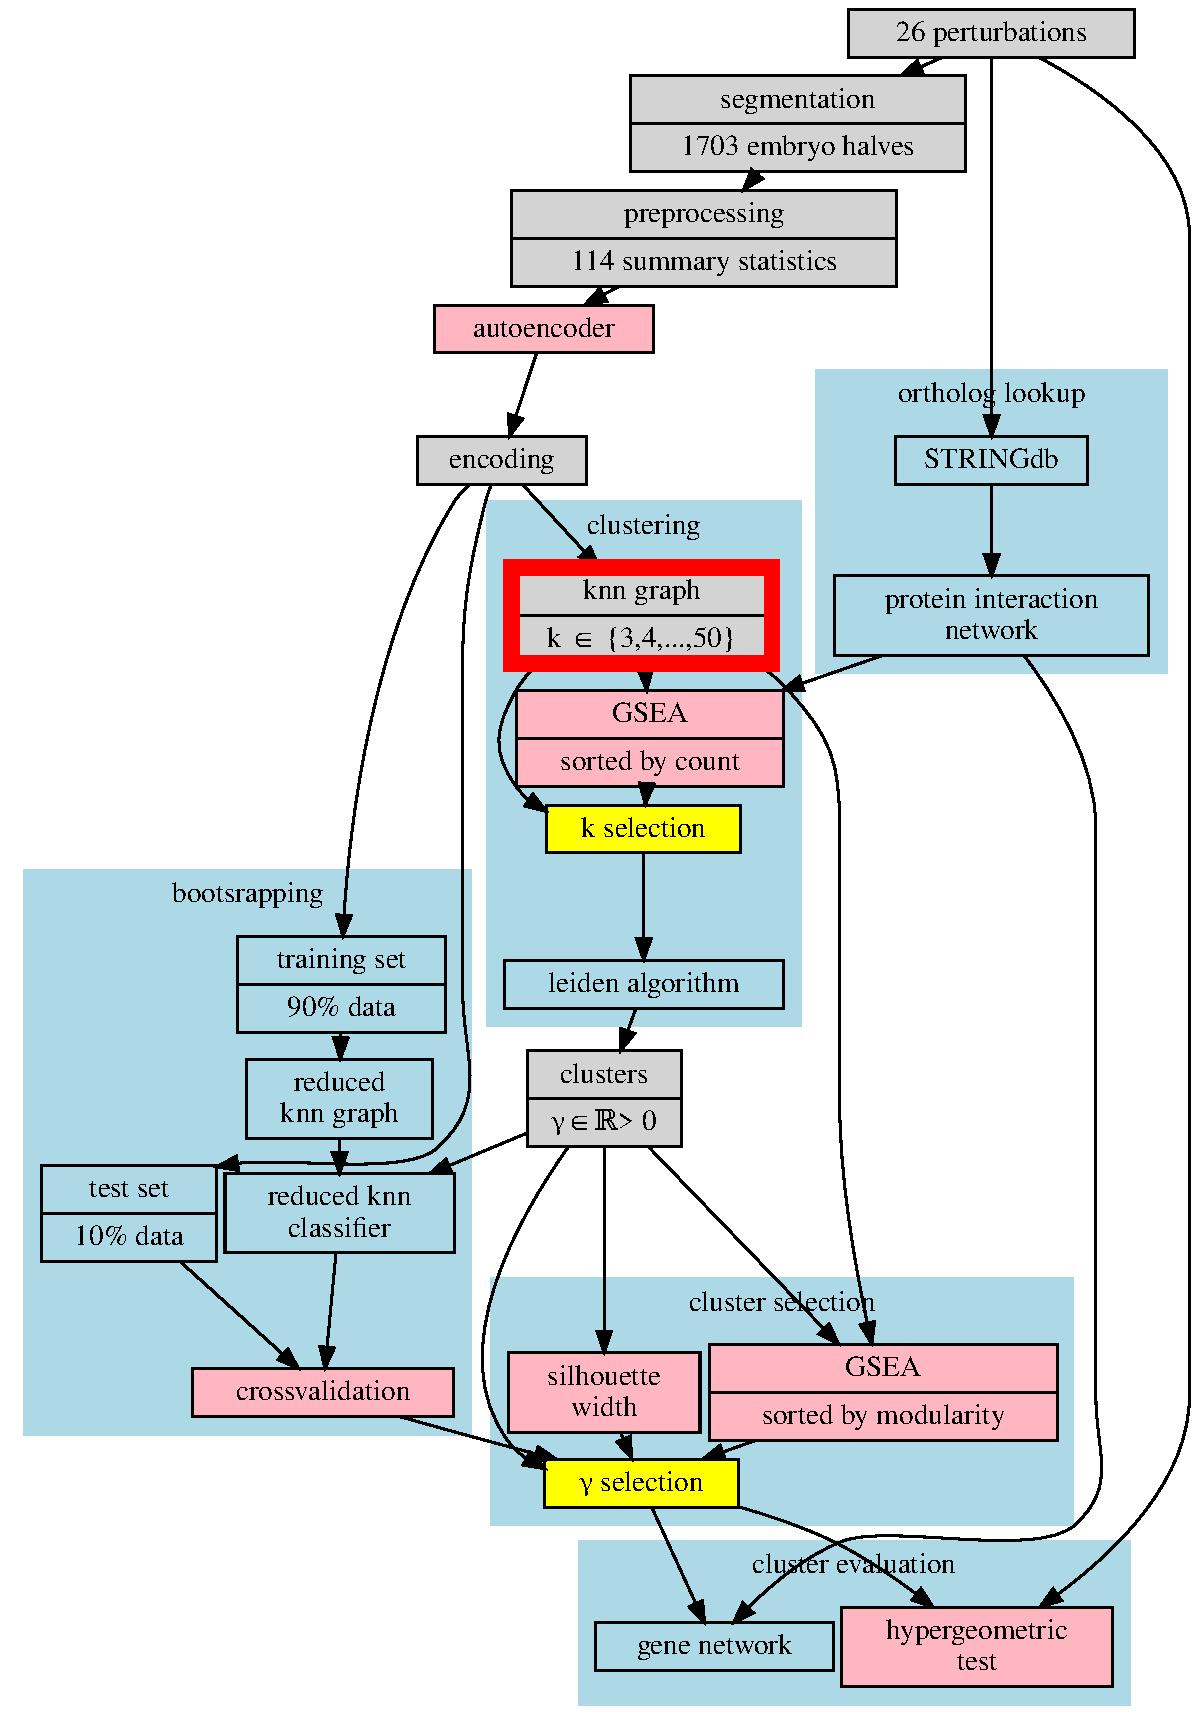
\includegraphics[width=\textwidth]{flowchart/knn.pdf}
		\end{column}
		\begin{column}{0.80\textwidth}
			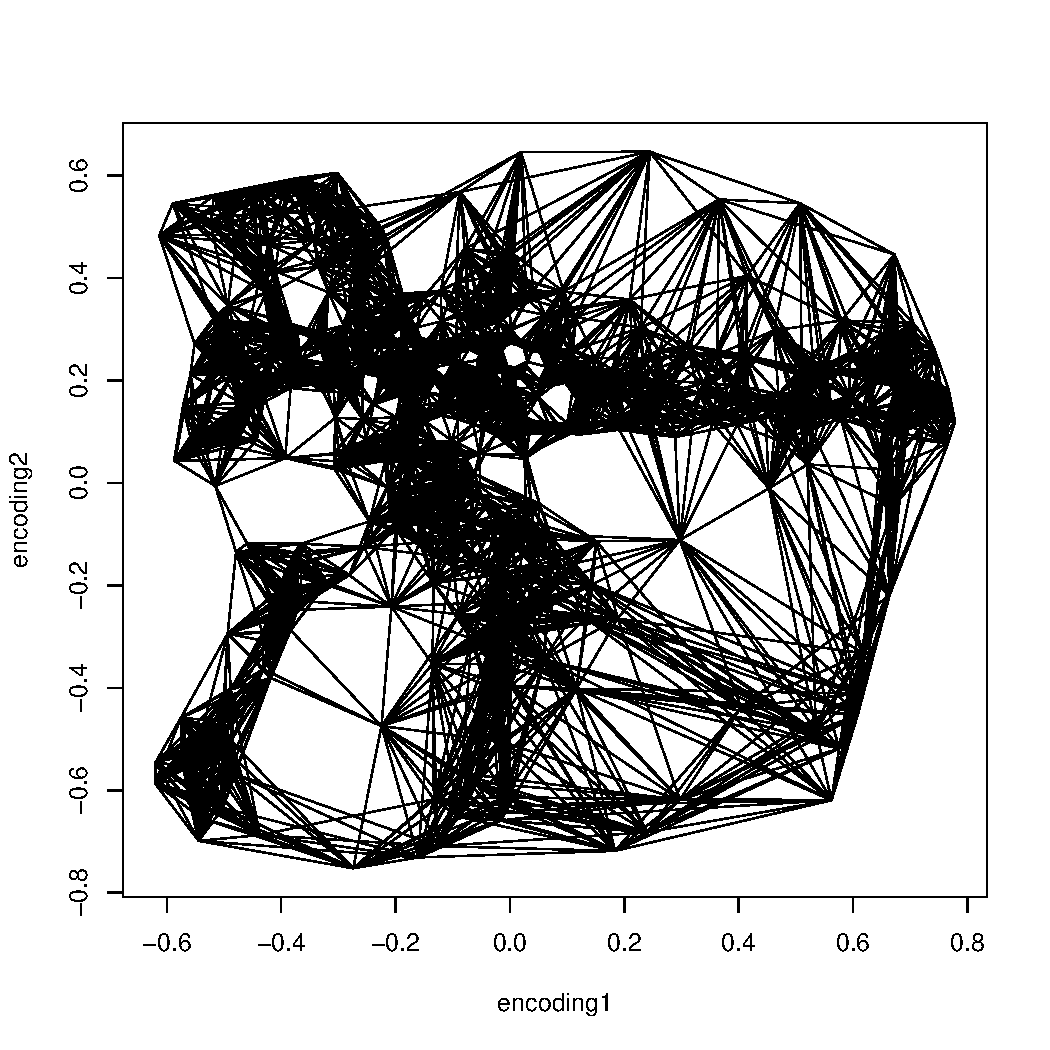
\includegraphics[width=\textwidth]{knn.pdf}
		\end{column}
	\end{columns}
}

\frame{
	\frametitle{}
	\begin{columns}
		\begin{column}{0.50\textwidth}
			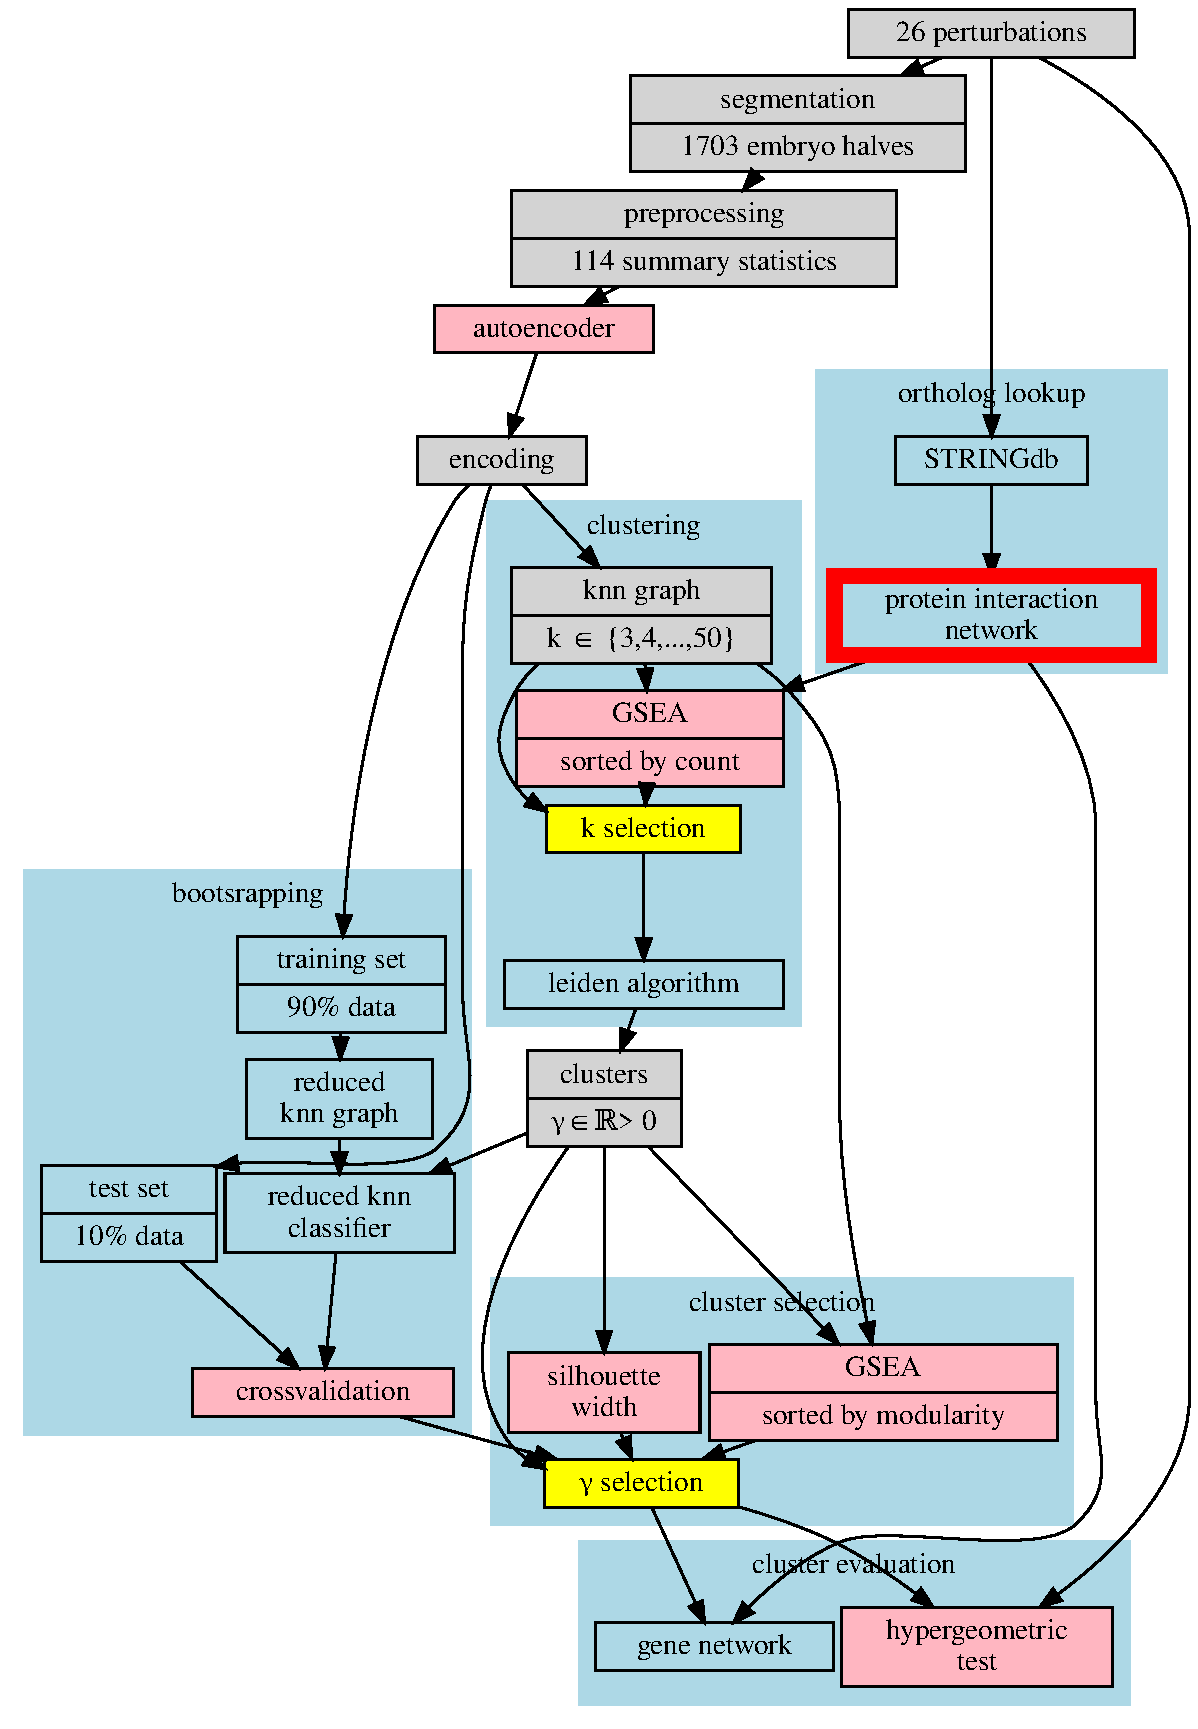
\includegraphics[width=\textwidth]{flowchart/prot.pdf}
		\end{column}
		\begin{column}{0.50\textwidth}
			I obtained orthologs from \textit{M. musculus} and \textit{H. sapiens} from ENSEMBL. I used STRINGdb to obtain known protein interactions.
		\end{column}
	\end{columns}
}


\frame{
	\frametitle{}
	\begin{columns}
		\begin{column}{0.50\textwidth}
			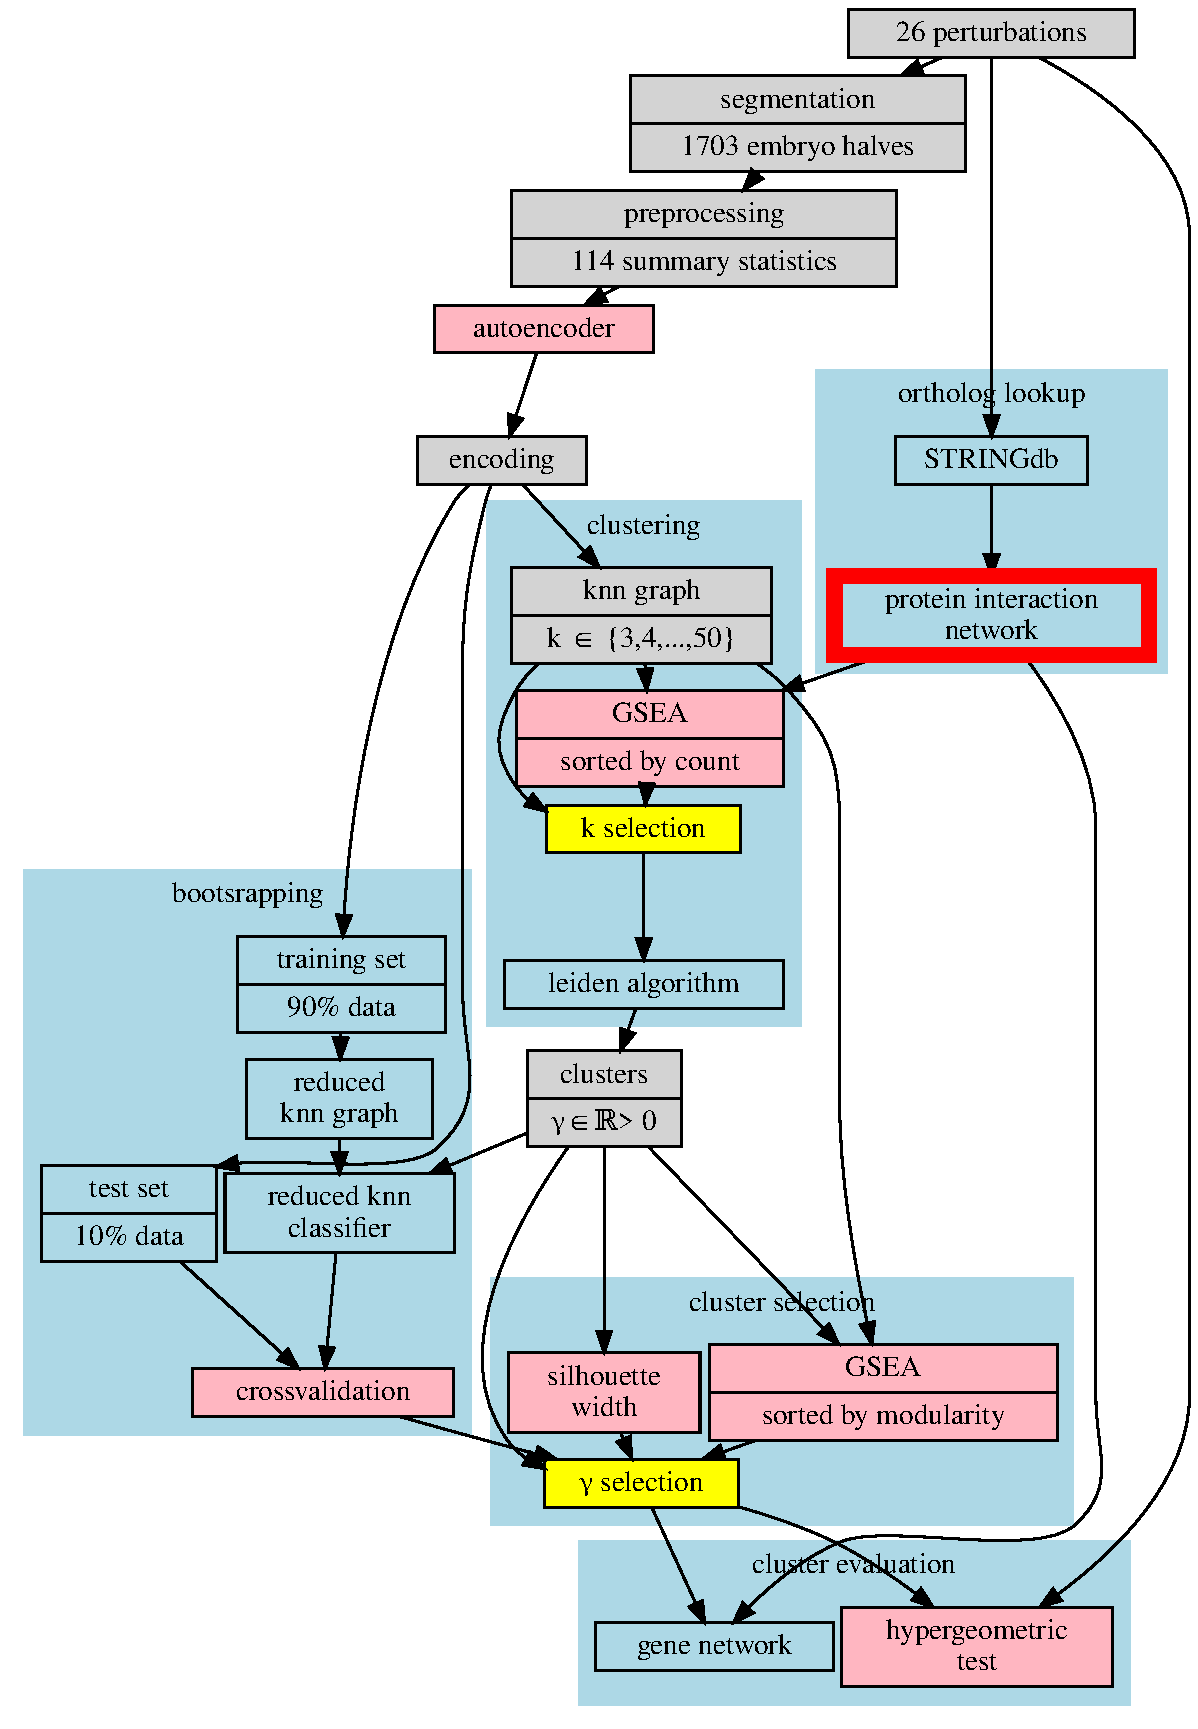
\includegraphics[width=\textwidth]{flowchart/prot.pdf}
		\end{column}
		\begin{column}{0.60\textwidth}
			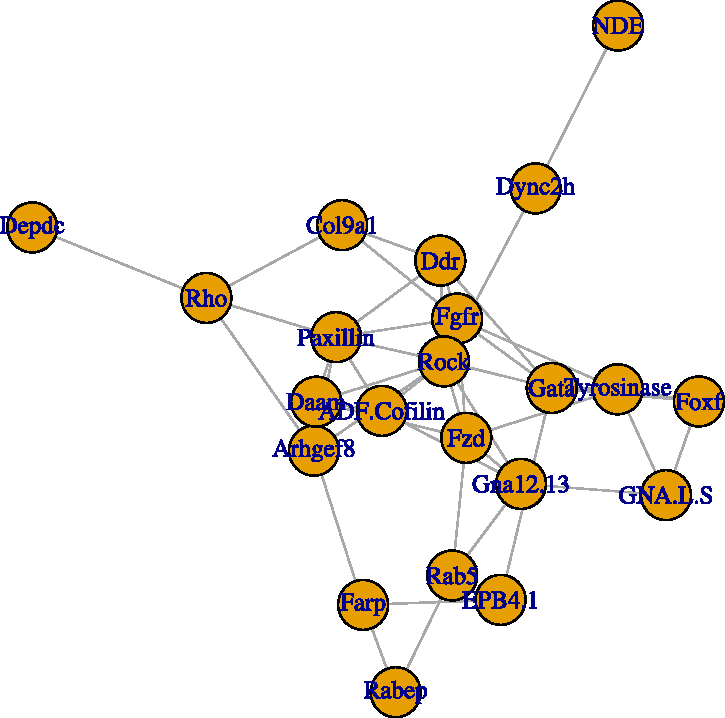
\includegraphics[width=\textwidth]{interactions_cropped.pdf}
		\end{column}
	\end{columns}
}

\frame{
	\frametitle{}
	\begin{columns}
		\begin{column}{0.50\textwidth}
			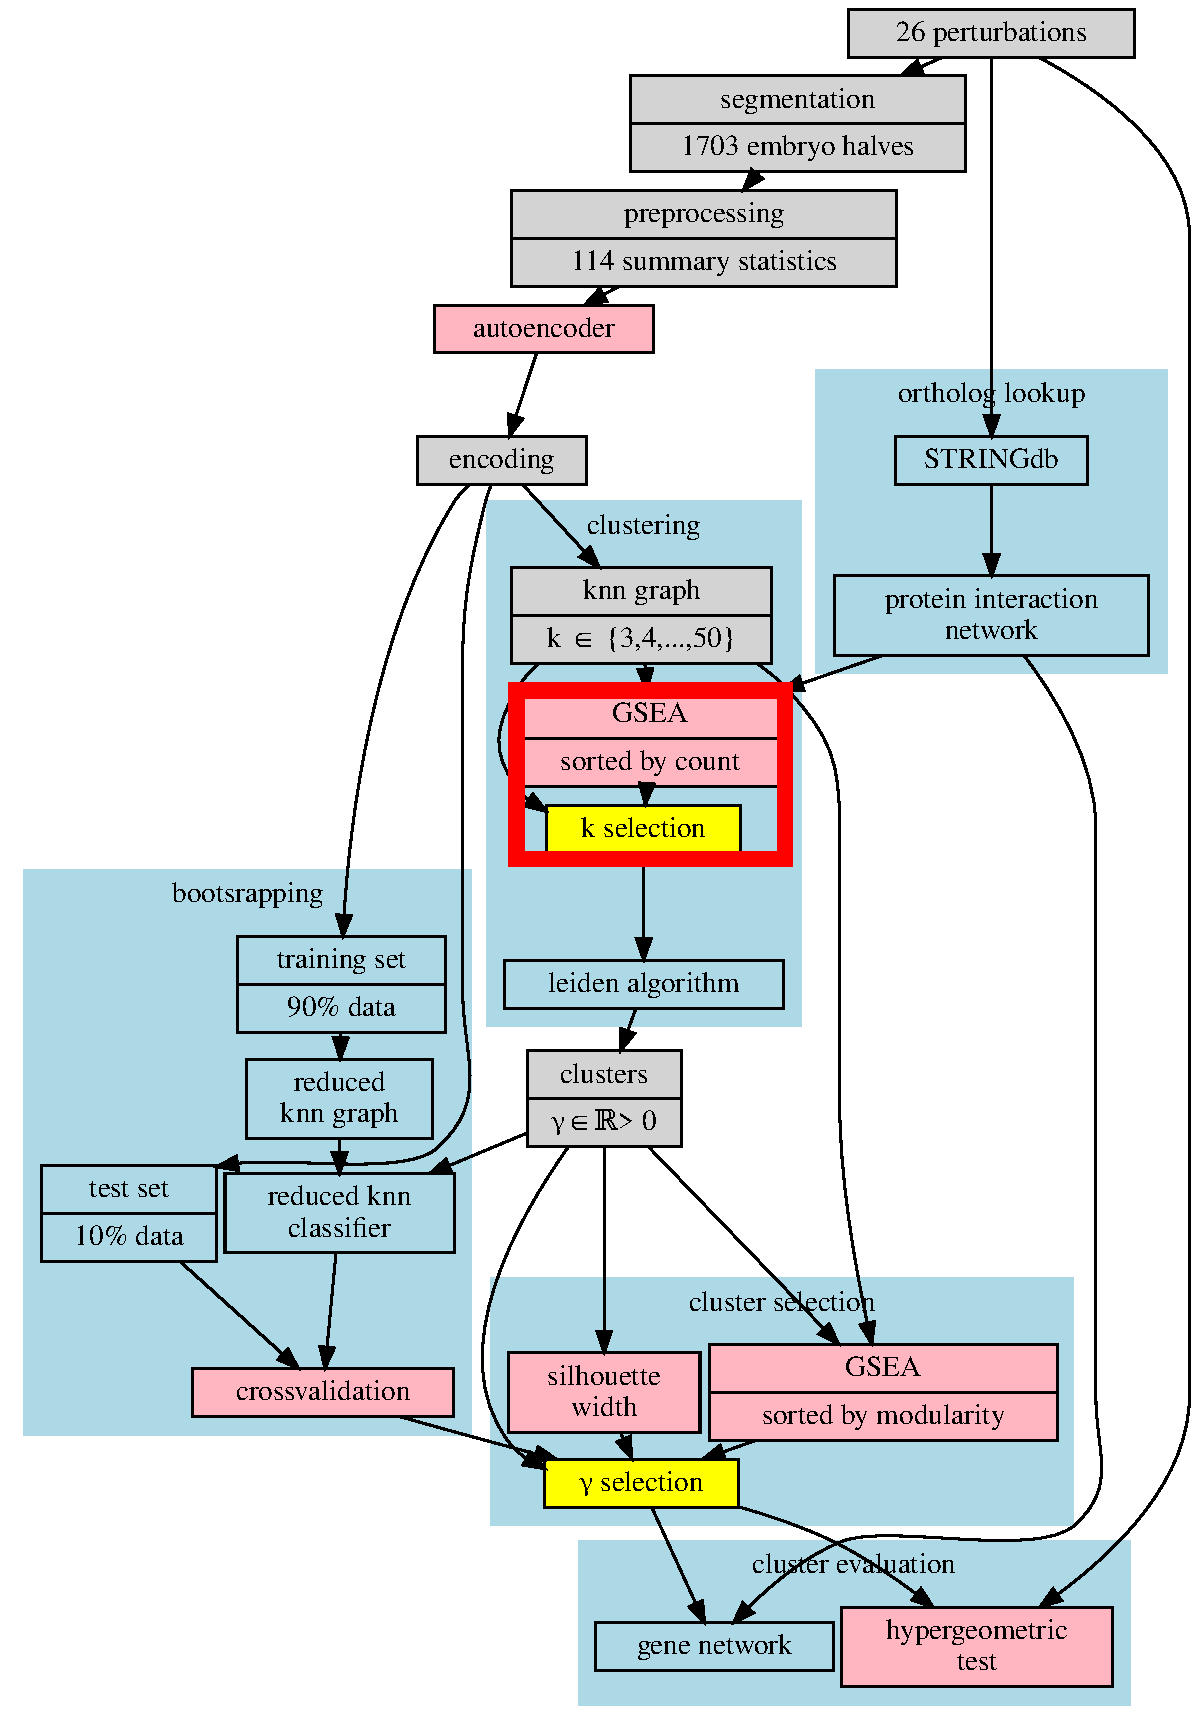
\includegraphics[width=\textwidth]{flowchart/ksel.pdf}
		\end{column}
		\begin{column}{0.50\textwidth}
			The known protein interactions can be treated as a gene set for GSEA. Interactions can be ranked by edge count between embryos in two conditions. An enrichment score is calculated based on occurrence of known interactions near the top of the ranked list. An optimal k can be selected by maximizing enrichment score.
		\end{column}
	\end{columns}
}

\frame{
	\frametitle{}
	\begin{columns}
		\begin{column}{0.50\textwidth}
			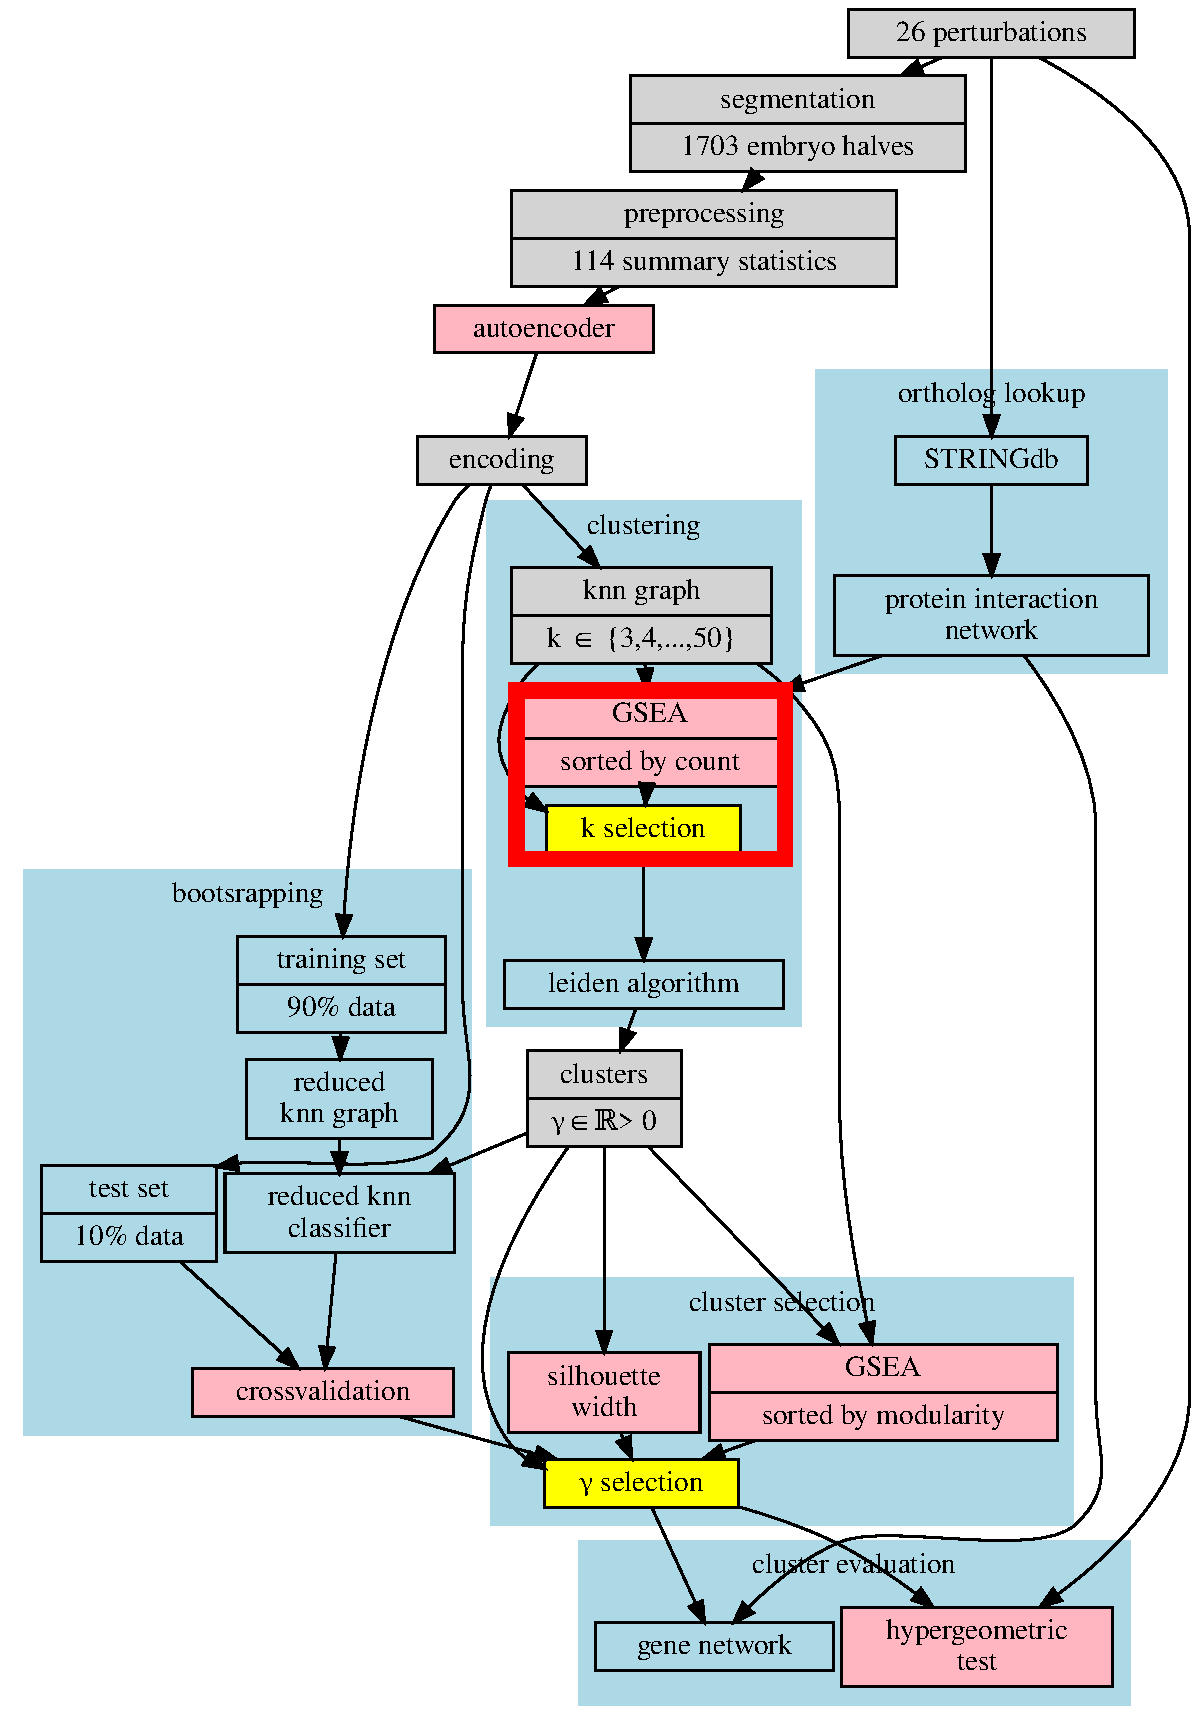
\includegraphics[width=\textwidth]{flowchart/ksel.pdf}
		\end{column}
		\begin{column}{0.40\textwidth}
			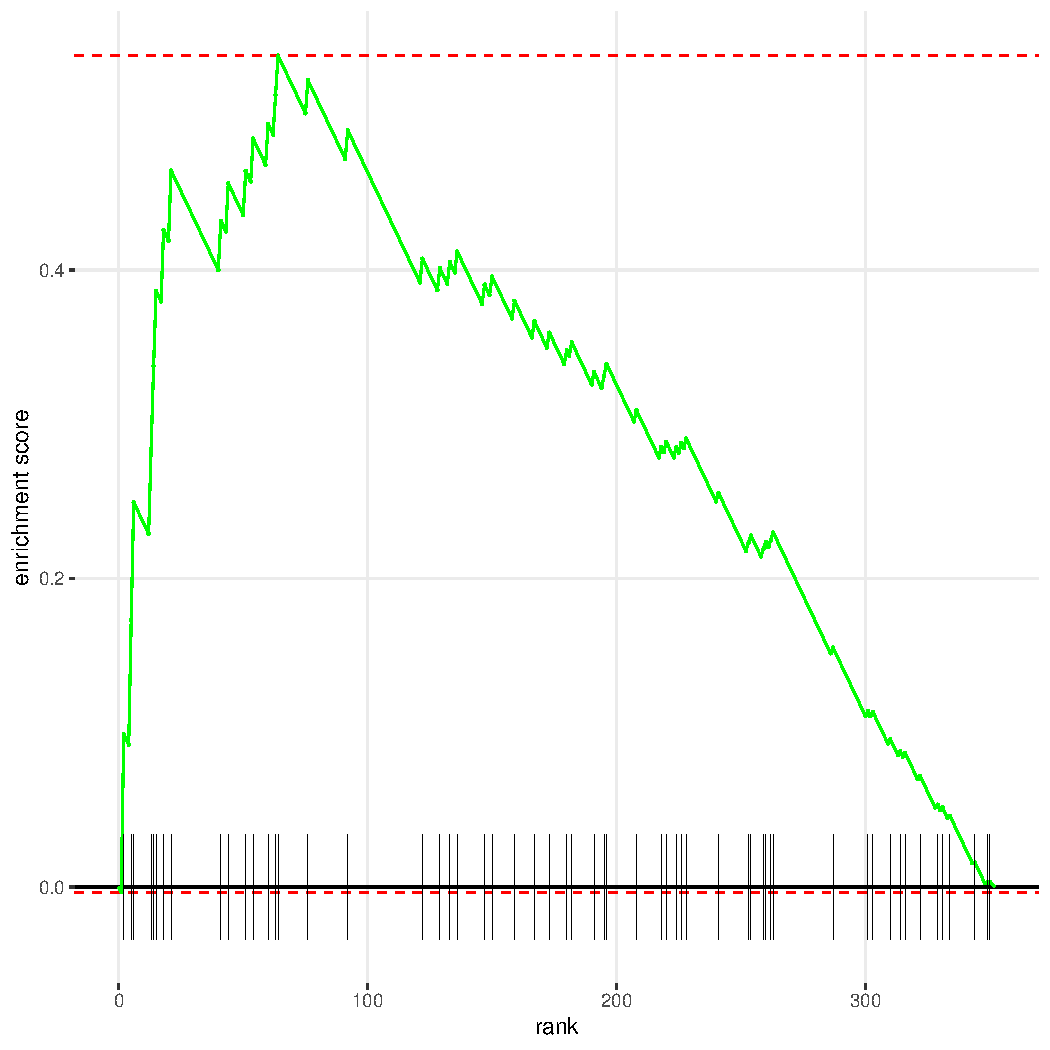
\includegraphics[width=\textwidth]{interaction_enrichment.pdf}
			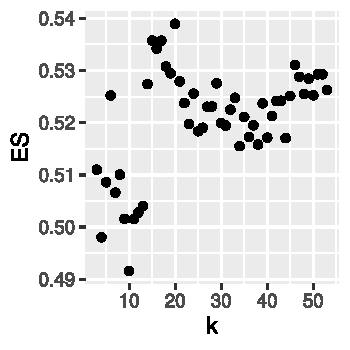
\includegraphics[width=\textwidth]{k_ES.pdf}
		\end{column}
	\end{columns}
}

\frame{
	\frametitle{}
	\begin{columns}
		\begin{column}{0.50\textwidth}
			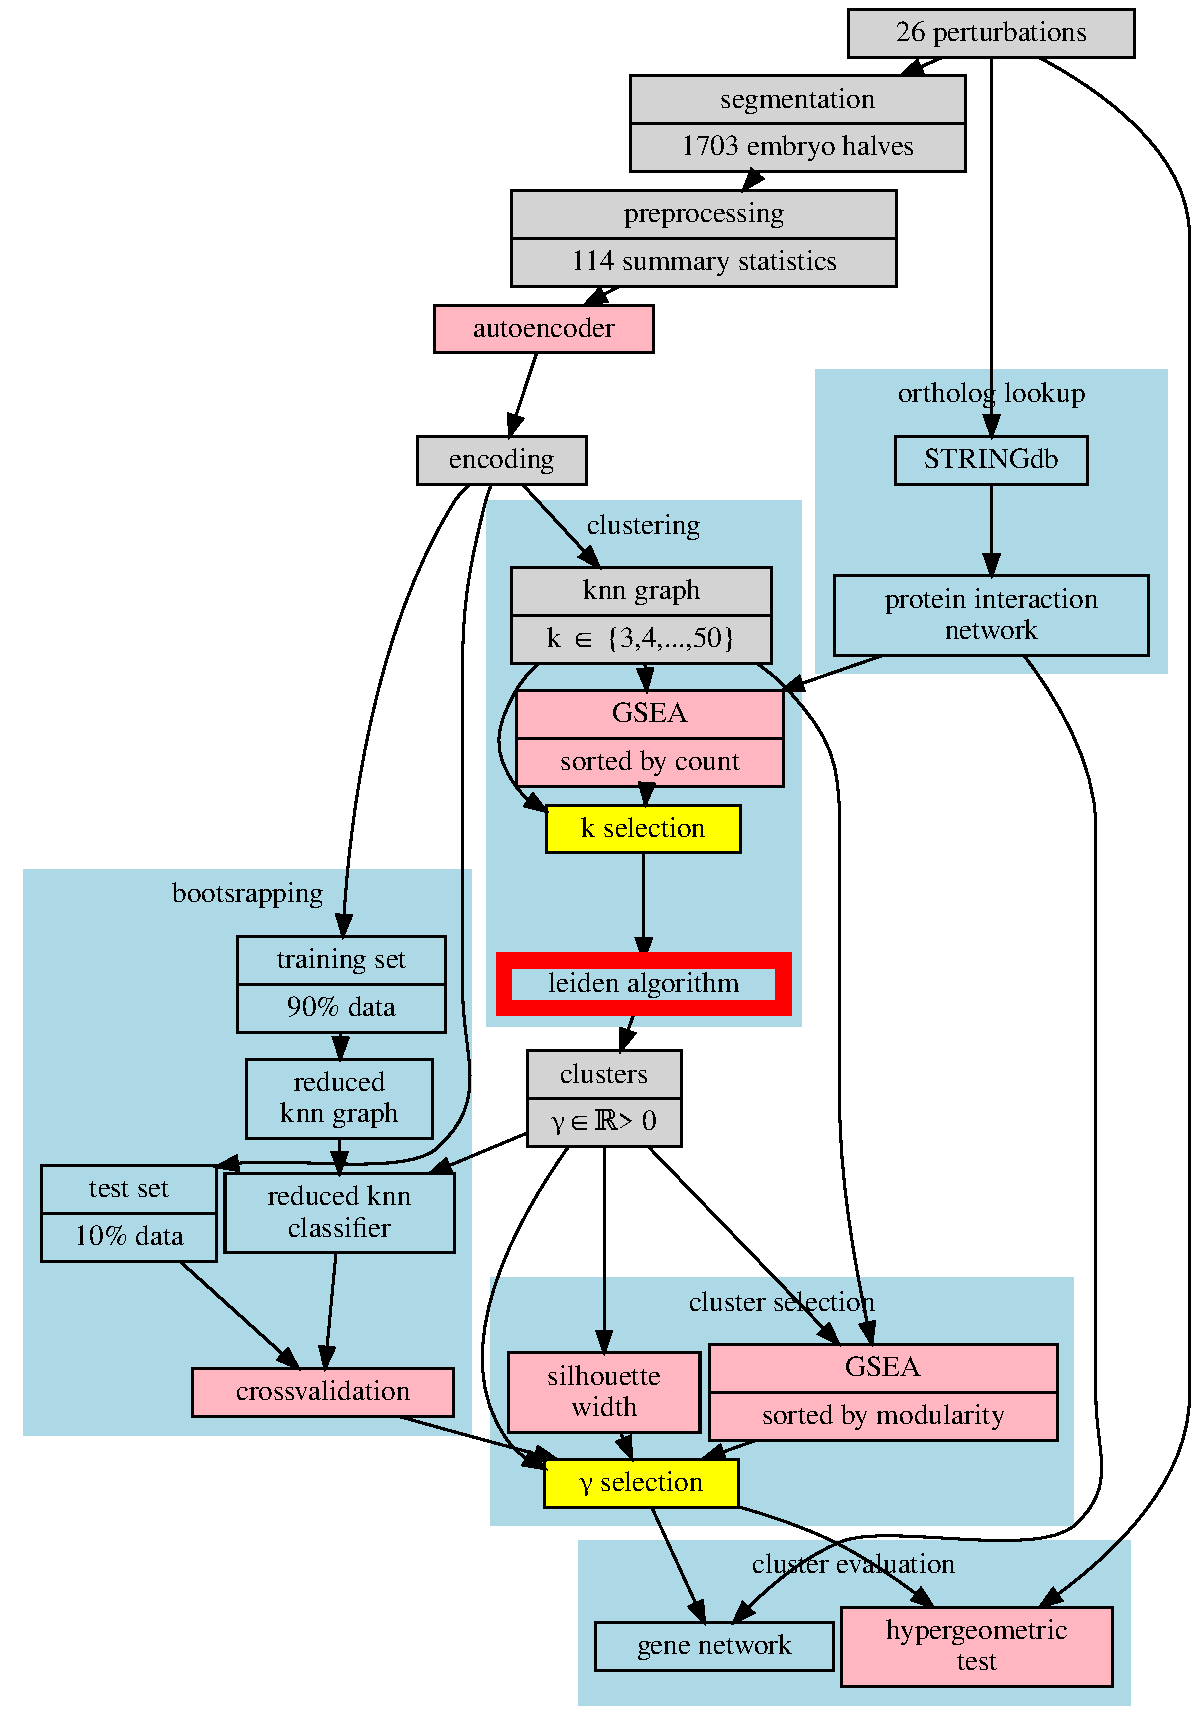
\includegraphics[width=\textwidth]{flowchart/leiden.pdf}
		\end{column}
		\begin{column}{0.50\textwidth}
			The leiden algorithm attempts to find a clustering that maximizes modularity $ H $ for a given graph and resolution $ \gamma $.  Modularity is defined as $$ H = \frac{1}{2m}\sum_{c}( \,e_c - \gamma\frac{K_c^2}{2m}) \, $$ where $m$ is the average degree of the graph, $e_c$ is the number of edges in cluster $c$, and $K_c$ is the number of nodes in cluster $c$. This gives a measure of how well-connected clusters compared to expectation based on average degree of the graph and number of nodes in a cluster. A higher $\gamma$ results in more clusters.
		\end{column}
	\end{columns}
}

\frame{
	\frametitle{}
	\begin{columns}
		\begin{column}{0.50\textwidth}
			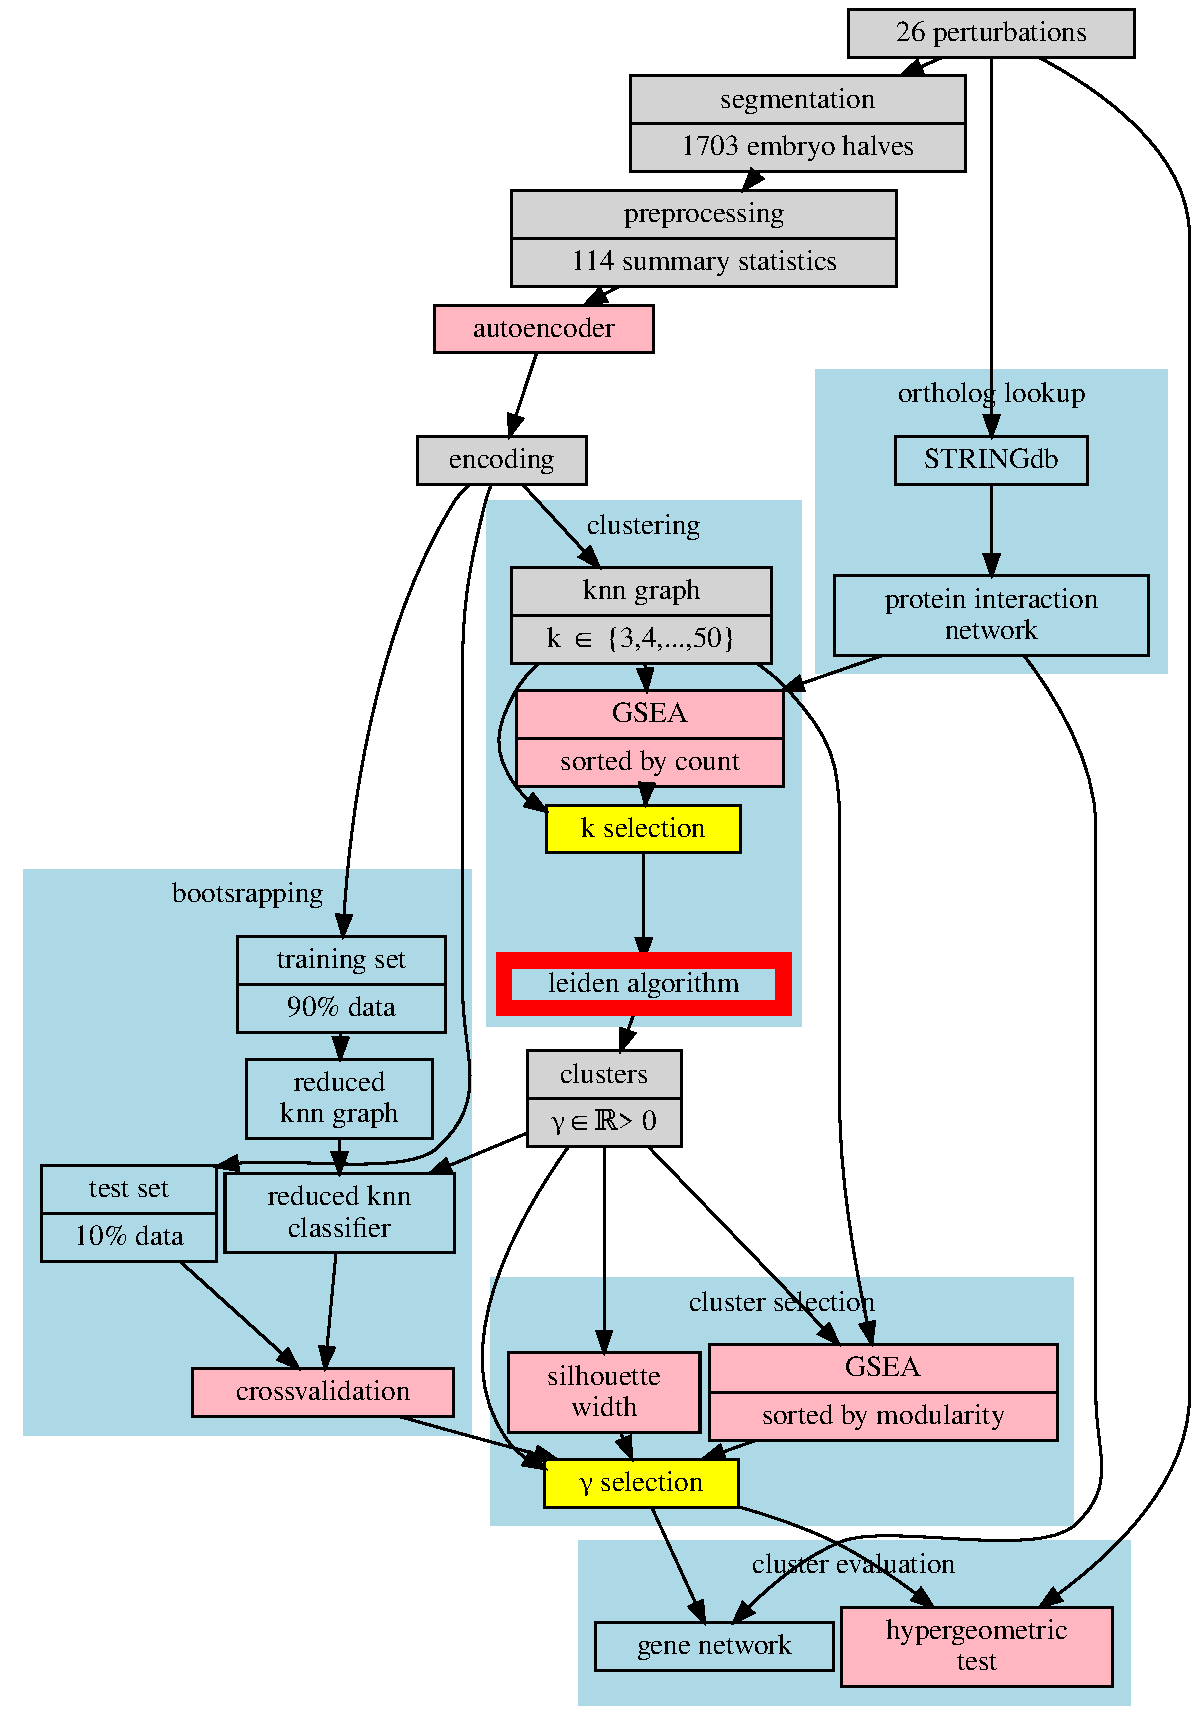
\includegraphics[width=\textwidth]{flowchart/leiden.pdf}
		\end{column}
		\begin{column}{0.50\textwidth}
			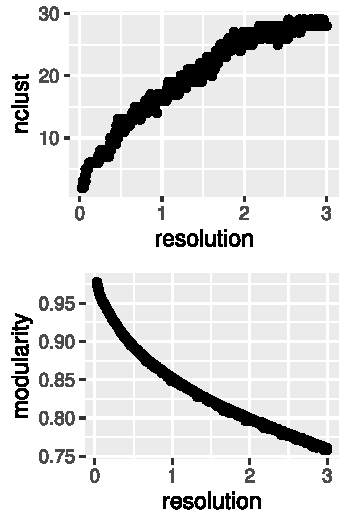
\includegraphics[width=\textwidth]{modularity.pdf}
		\end{column}
	\end{columns}
}

\frame{
	\frametitle{}
	\begin{columns}
		\begin{column}{0.50\textwidth}
			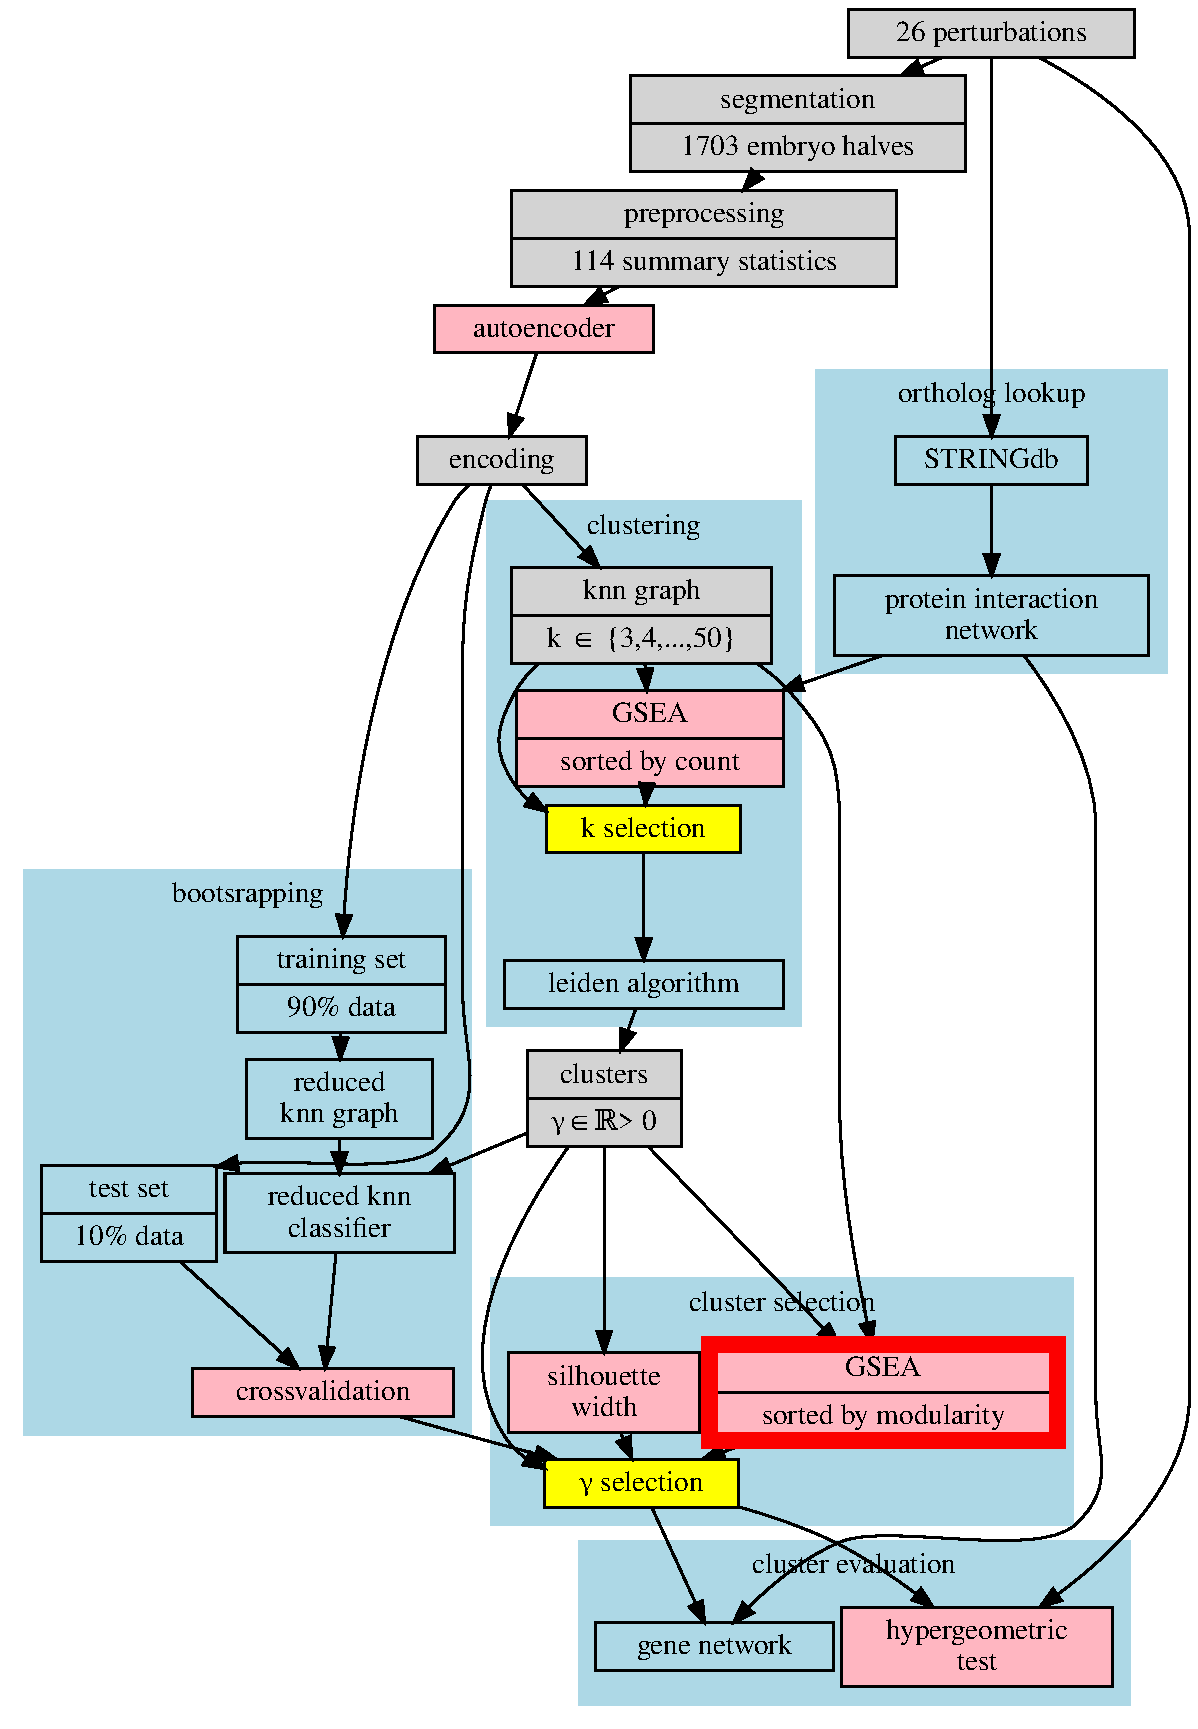
\includegraphics[width=\textwidth]{flowchart/gsea.pdf}
		\end{column}
		\begin{column}{0.50\textwidth}
			I obtained 1000 clusterings on random $\gamma$ values between 0.01 and 3. I assessed clustering by several metrics. I obtained an enrichment score from a second GSEA with interactions ranked by modularity of a subgraph consisting of only edges between two given conditions. 
		\end{column}
	\end{columns}
}

\frame{
	\frametitle{}
	\begin{columns}
		\begin{column}{0.50\textwidth}
			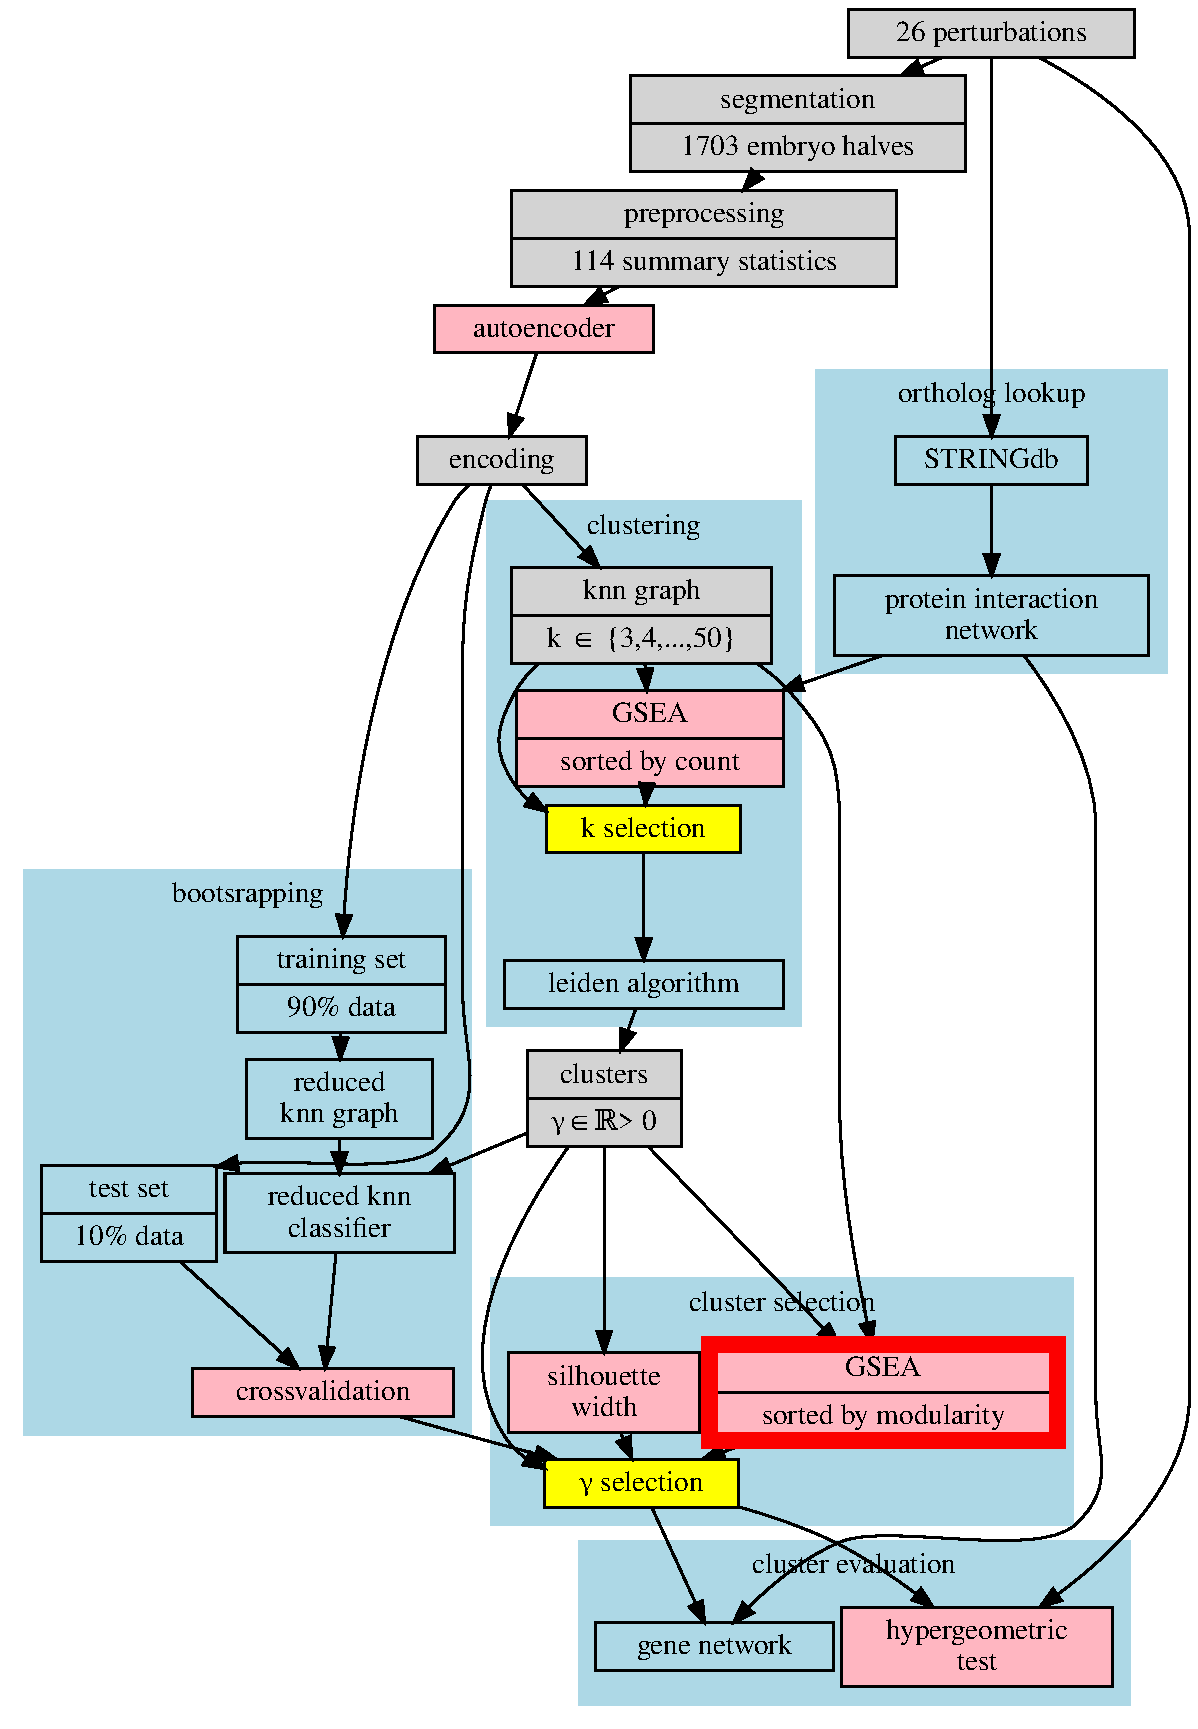
\includegraphics[width=\textwidth]{flowchart/gsea.pdf}
		\end{column}
		\begin{column}{0.50\textwidth}
			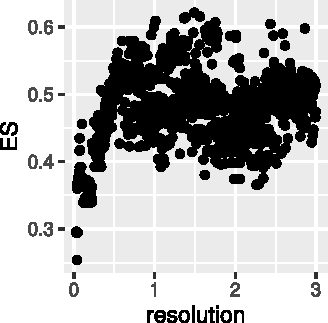
\includegraphics[width=0.5\textwidth]{ES.pdf}
			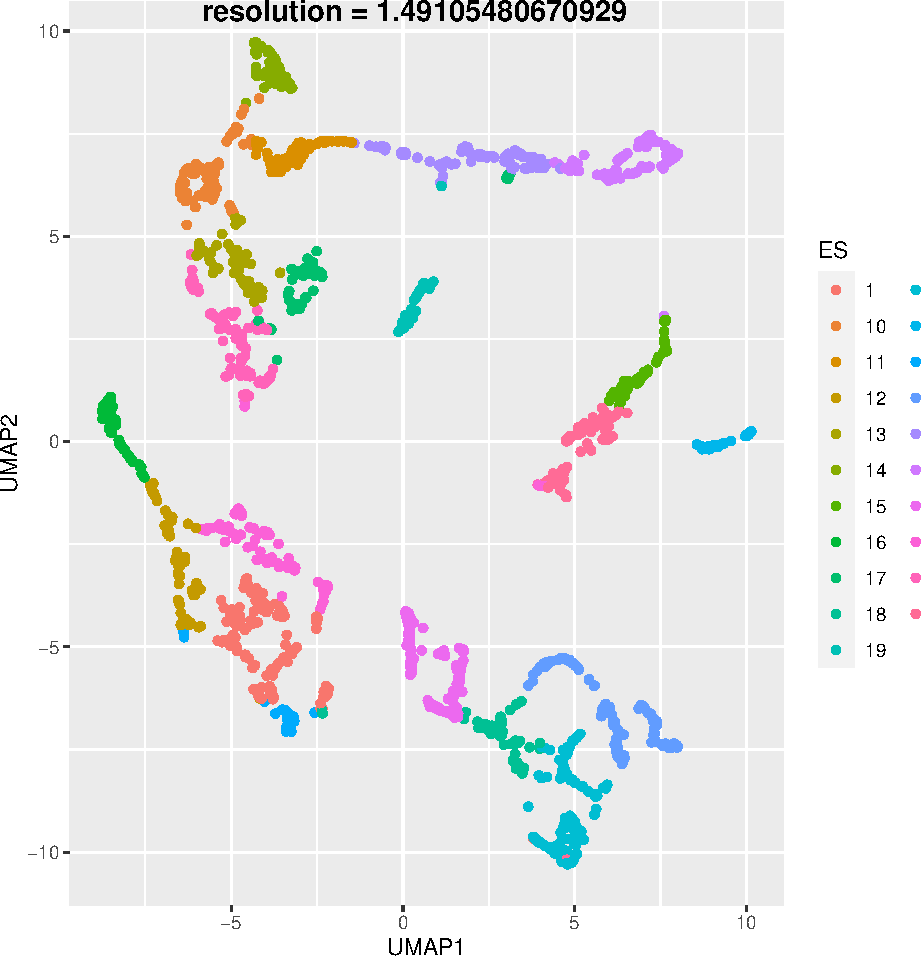
\includegraphics[width=\textwidth]{umap_ES.pdf}
		\end{column}
	\end{columns}
}

\frame{
	\frametitle{}
	\begin{columns}
		\begin{column}{0.50\textwidth}
			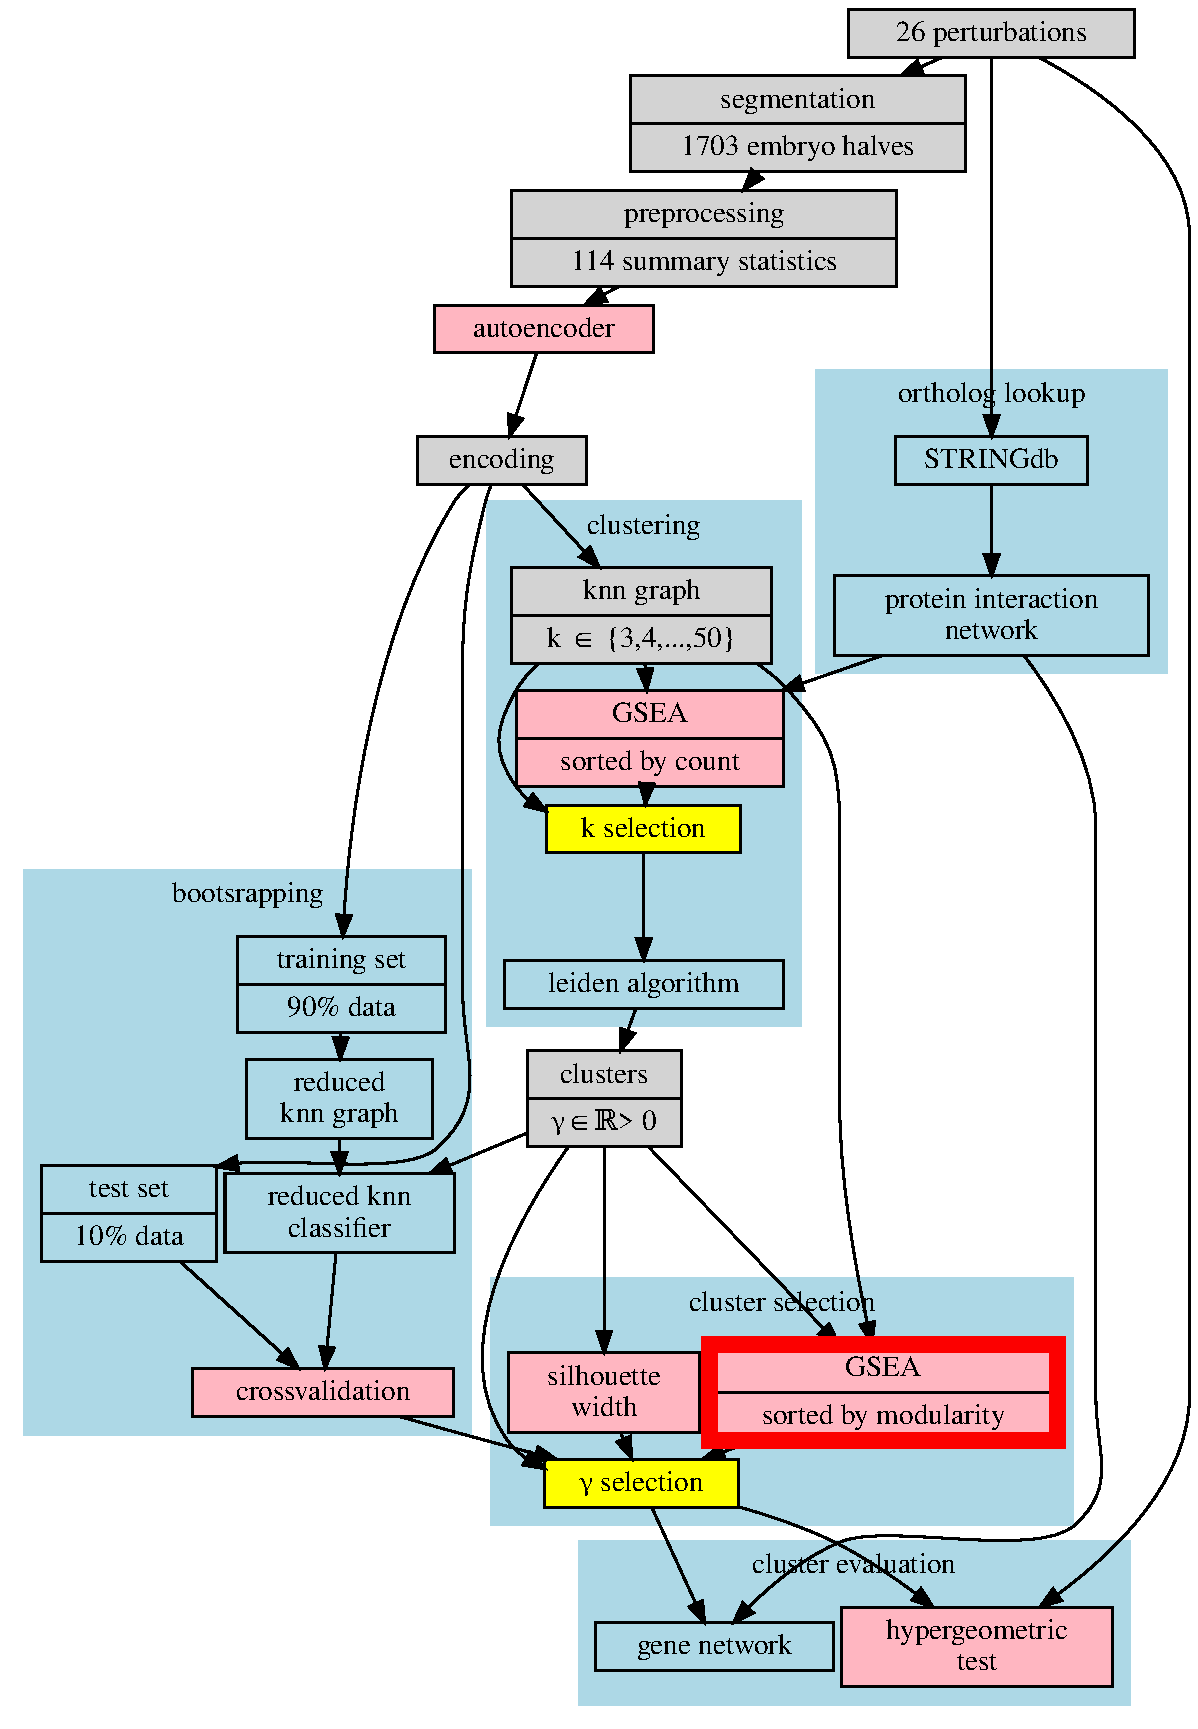
\includegraphics[width=\textwidth]{flowchart/gsea.pdf}
		\end{column}
		\begin{column}{0.50\textwidth}
			I used this same metric to construct a gene network. If an interaction has positive modularity the genes are considered connected. A recall score can be calculated by comparing this network to the protein interaction network. 
		\end{column}
	\end{columns}
}


\frame{
	\frametitle{}
	\begin{columns}
		\begin{column}{0.50\textwidth}
			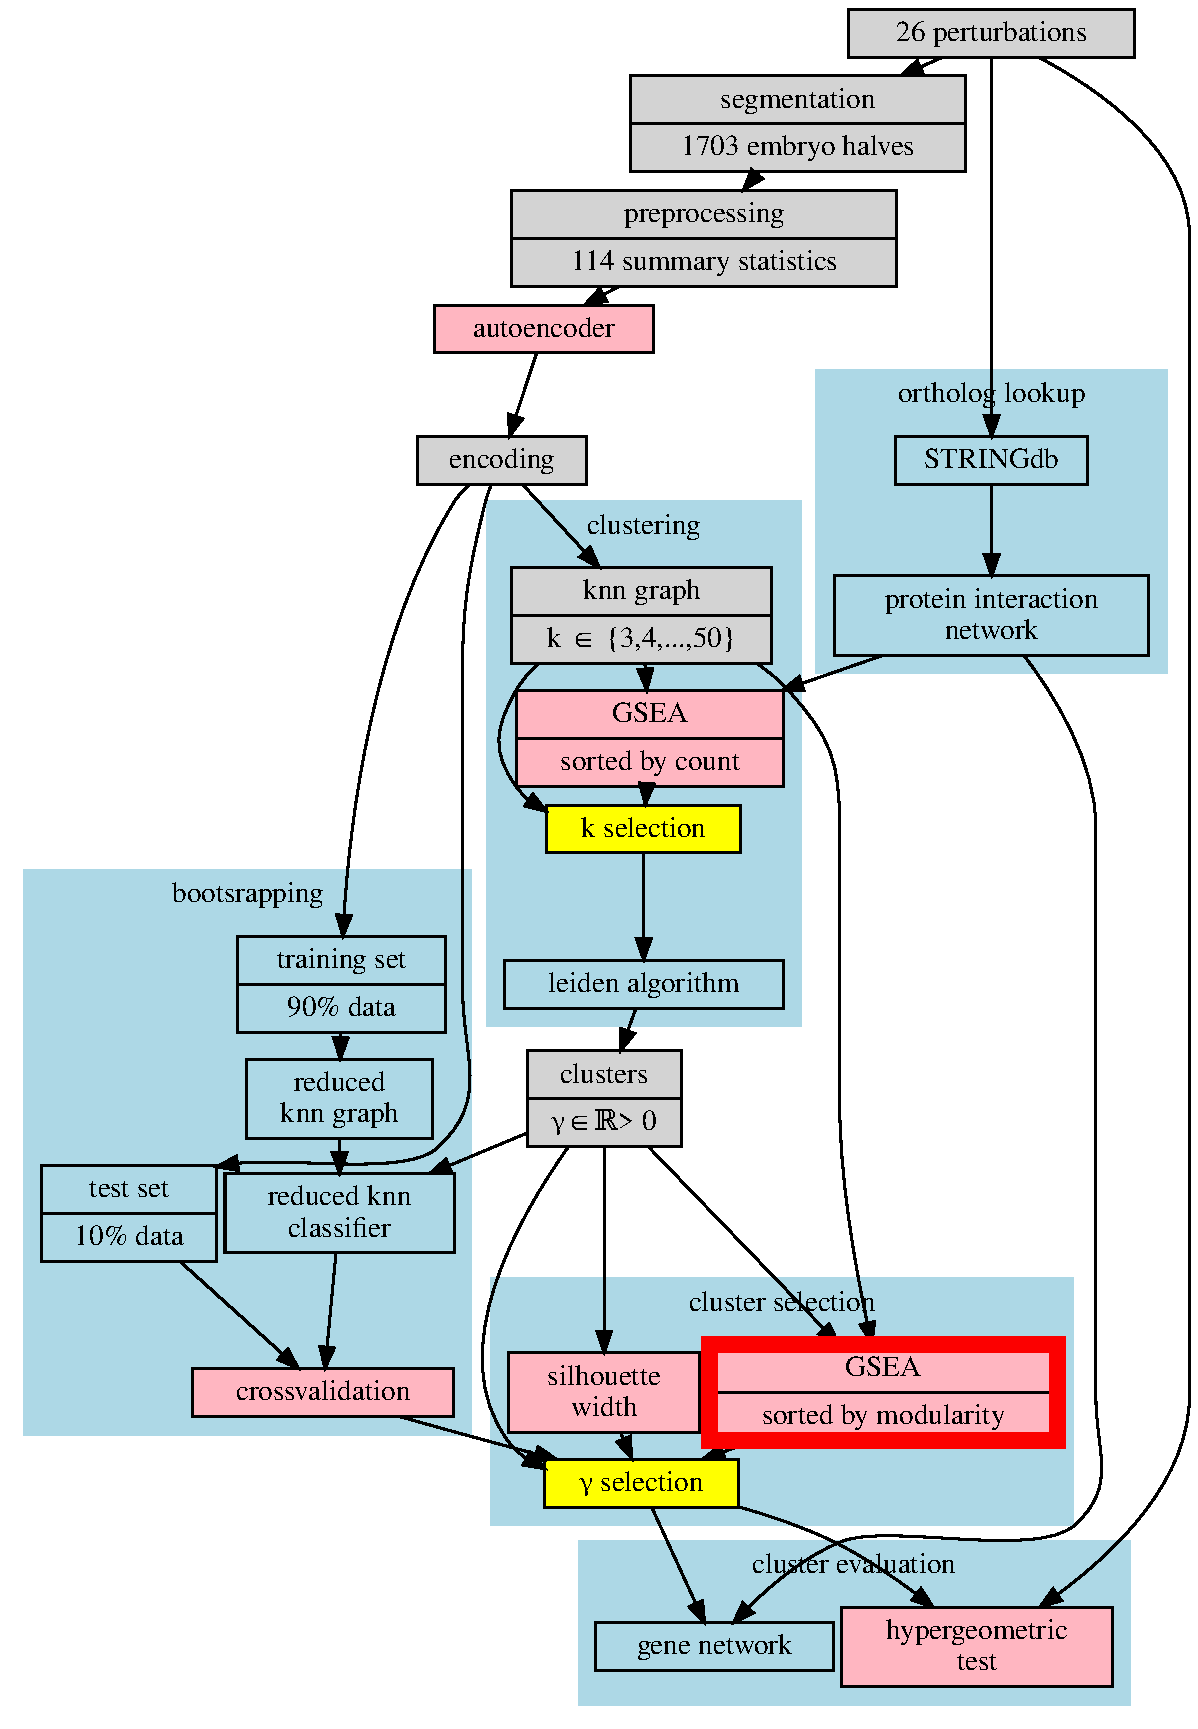
\includegraphics[width=\textwidth]{flowchart/gsea.pdf}
		\end{column}
		\begin{column}{0.50\textwidth}
			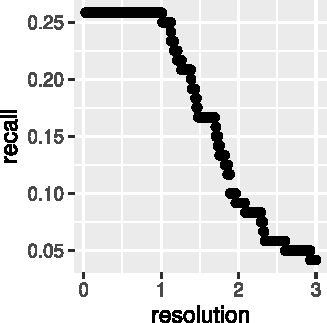
\includegraphics[width=0.5\textwidth]{recall.pdf}
			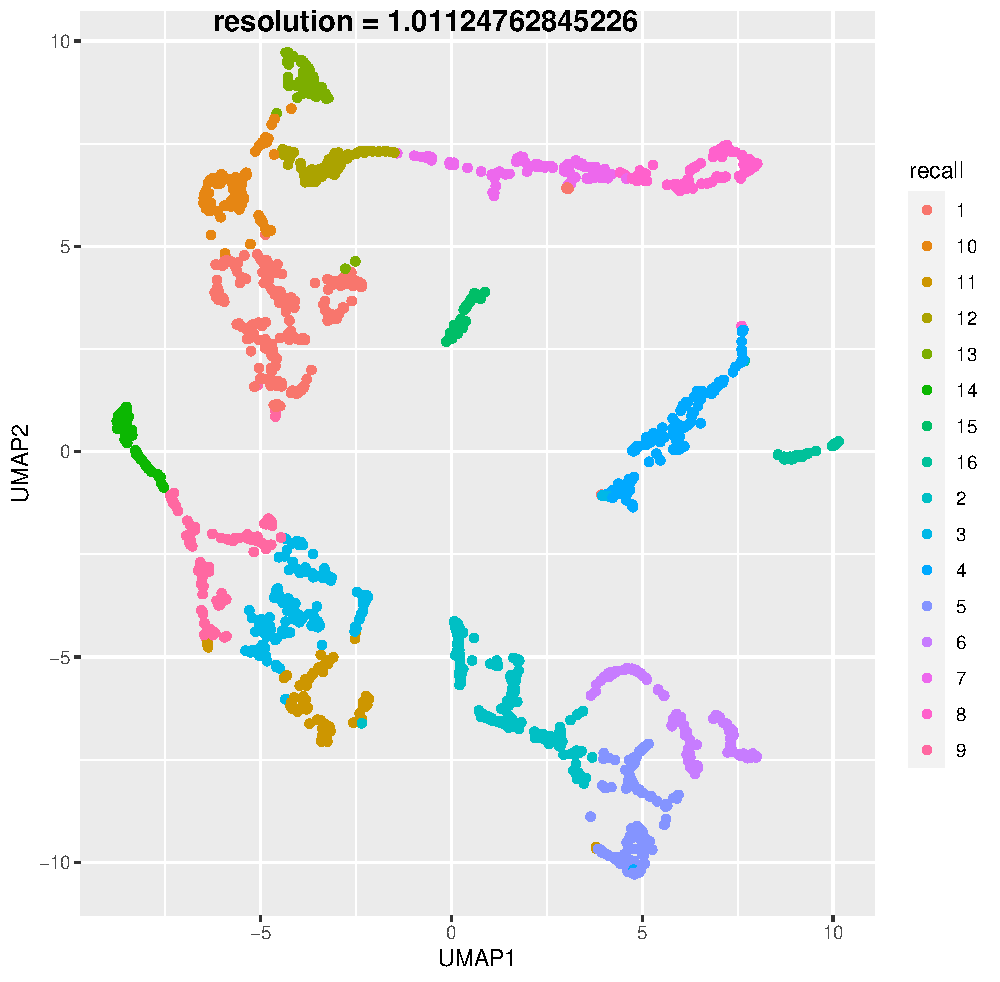
\includegraphics[width=\textwidth]{umap_recall.pdf}
		\end{column}
	\end{columns}
}

\frame{
	\frametitle{}
	\begin{columns}
		\begin{column}{0.50\textwidth}
			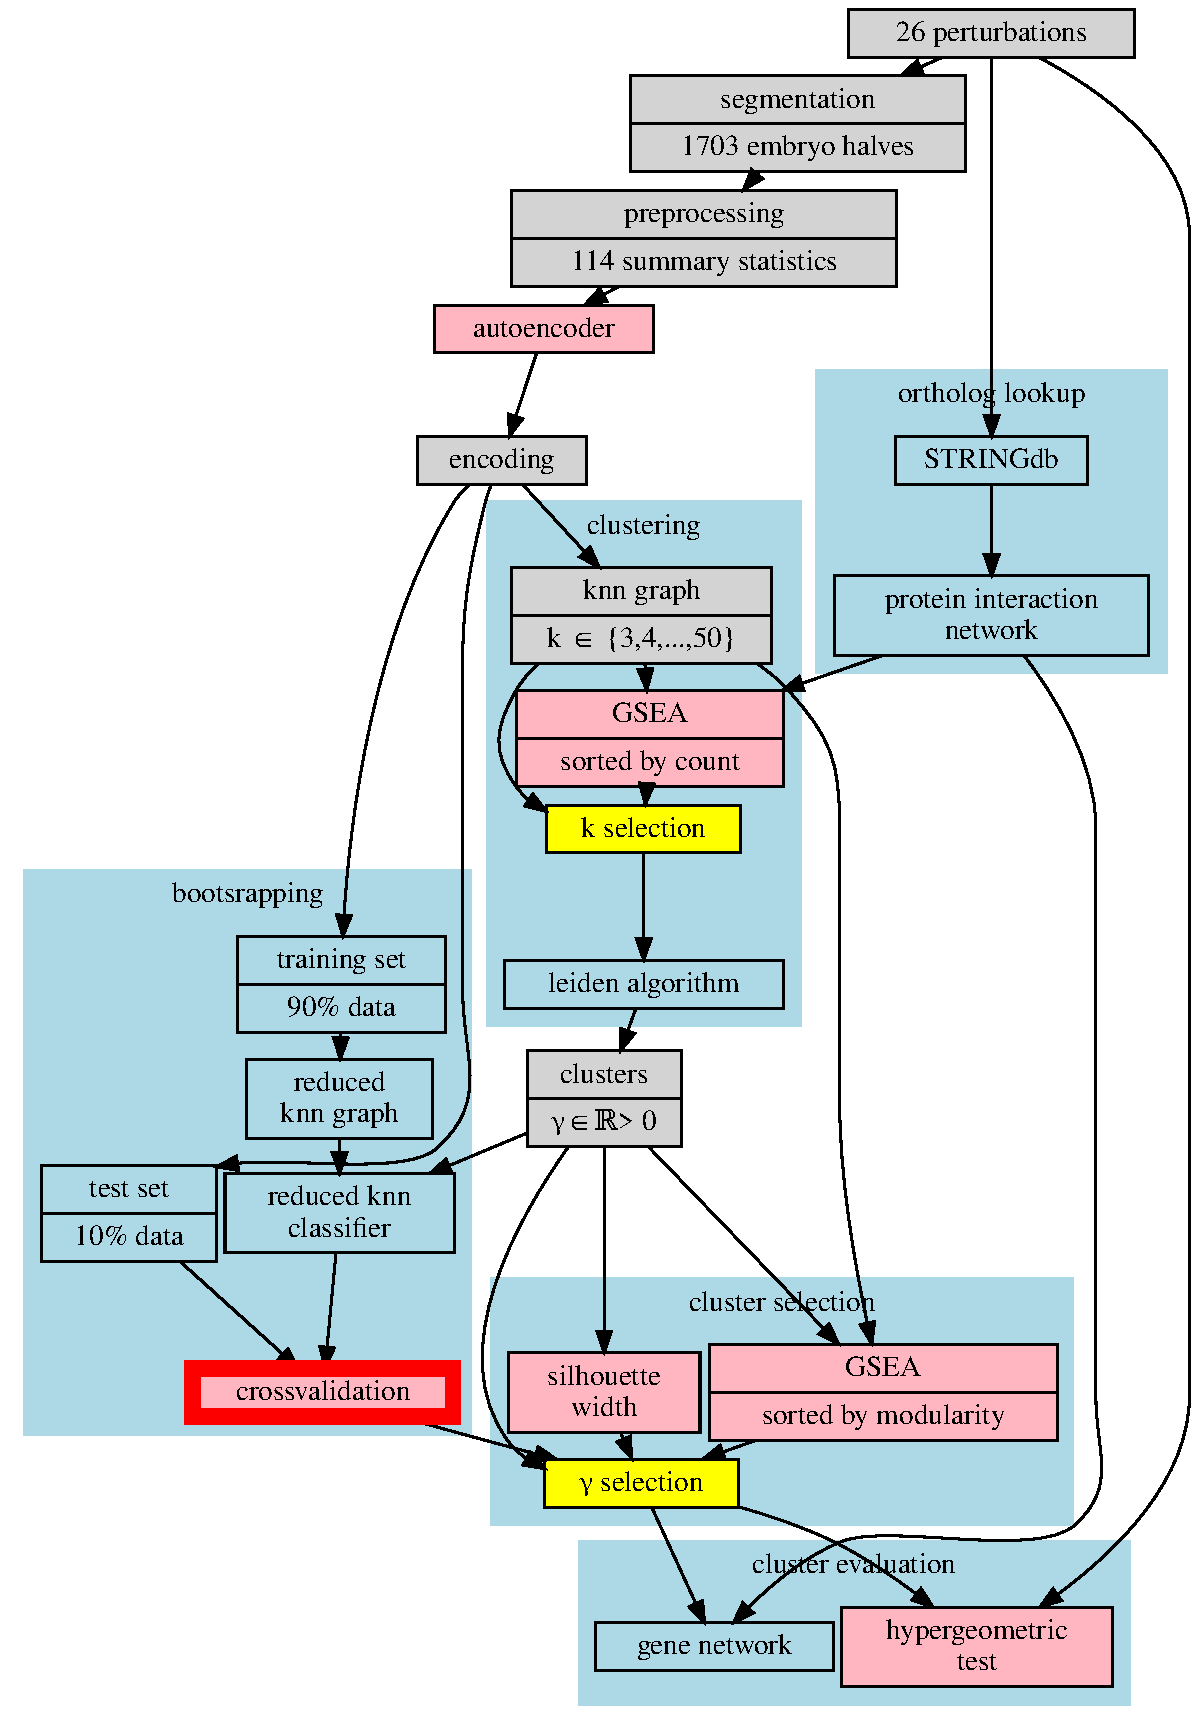
\includegraphics[width=\textwidth]{flowchart/cv.pdf}
		\end{column}
		\begin{column}{0.50\textwidth}
			I used this same metric to construct a gene network. If an interaction has positive modularity the genes are considered connected. A recall score can be calculated by comparing this network to the protein interaction network. $-log_2 error$ is calculated by building a kNN classifier for the clusters from a subset of the data and repeating for 1000 permutations. 
		\end{column}
	\end{columns}
}

\frame{
	\frametitle{}
	\begin{columns}
		\begin{column}{0.50\textwidth}
			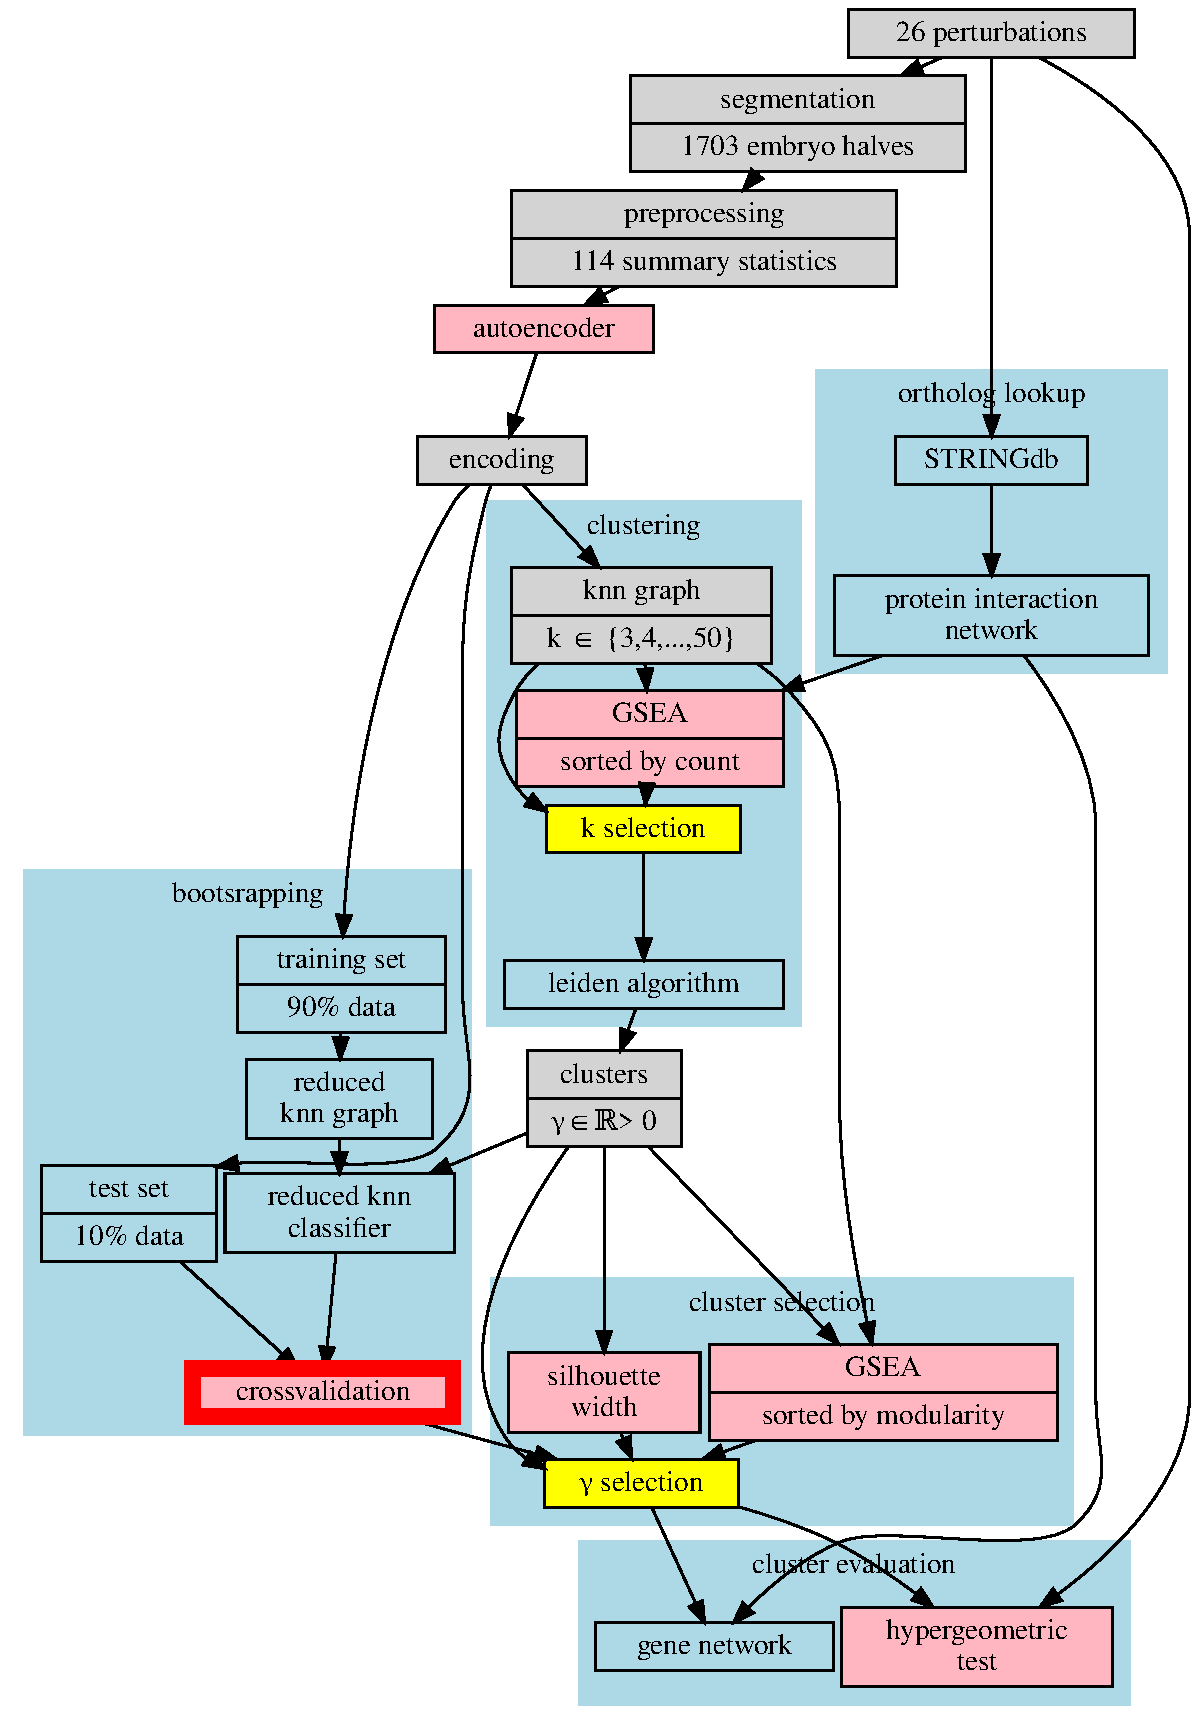
\includegraphics[width=\textwidth]{flowchart/cv.pdf}
		\end{column}
		\begin{column}{0.50\textwidth}
			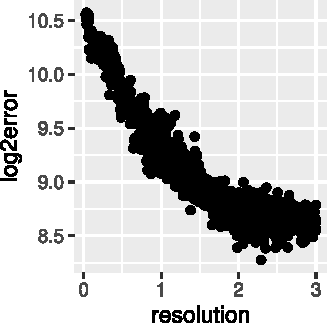
\includegraphics[width=0.5\textwidth]{err.pdf}
			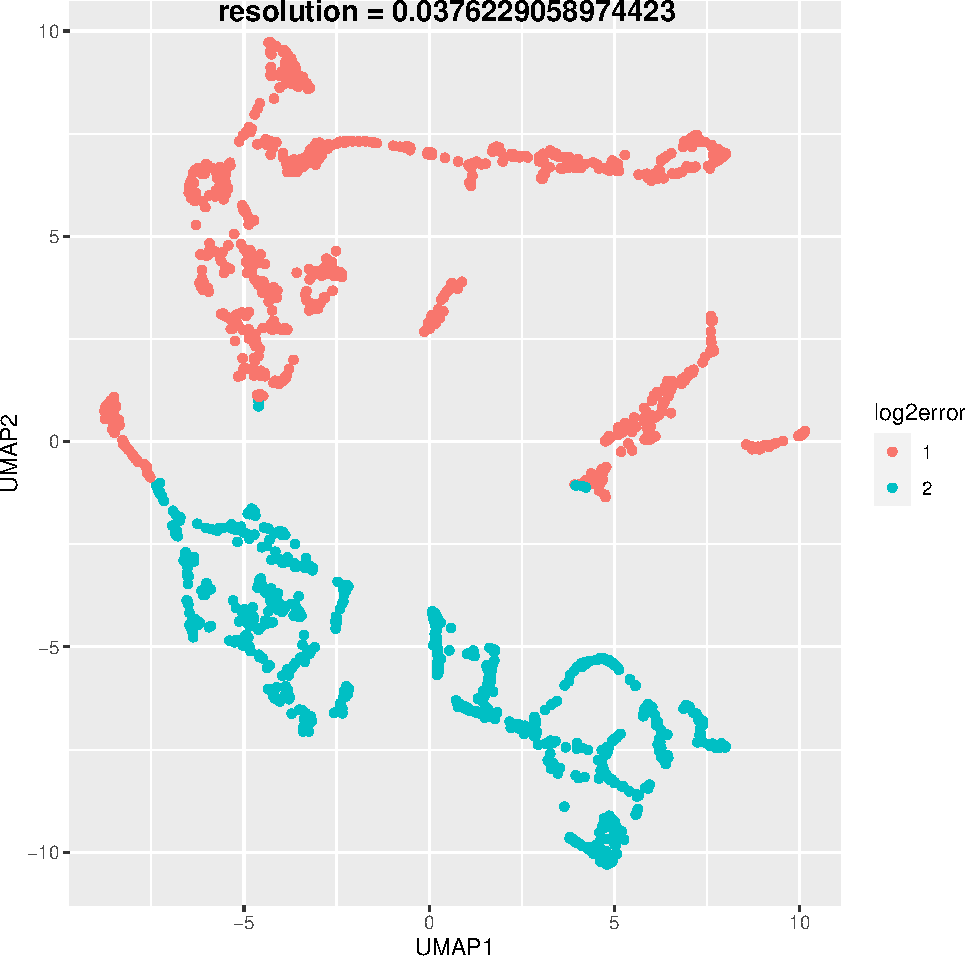
\includegraphics[width=\textwidth]{umap_err.pdf}
		\end{column}
	\end{columns}
}

\frame{
	\frametitle{}
	\begin{columns}
		\begin{column}{0.50\textwidth}
			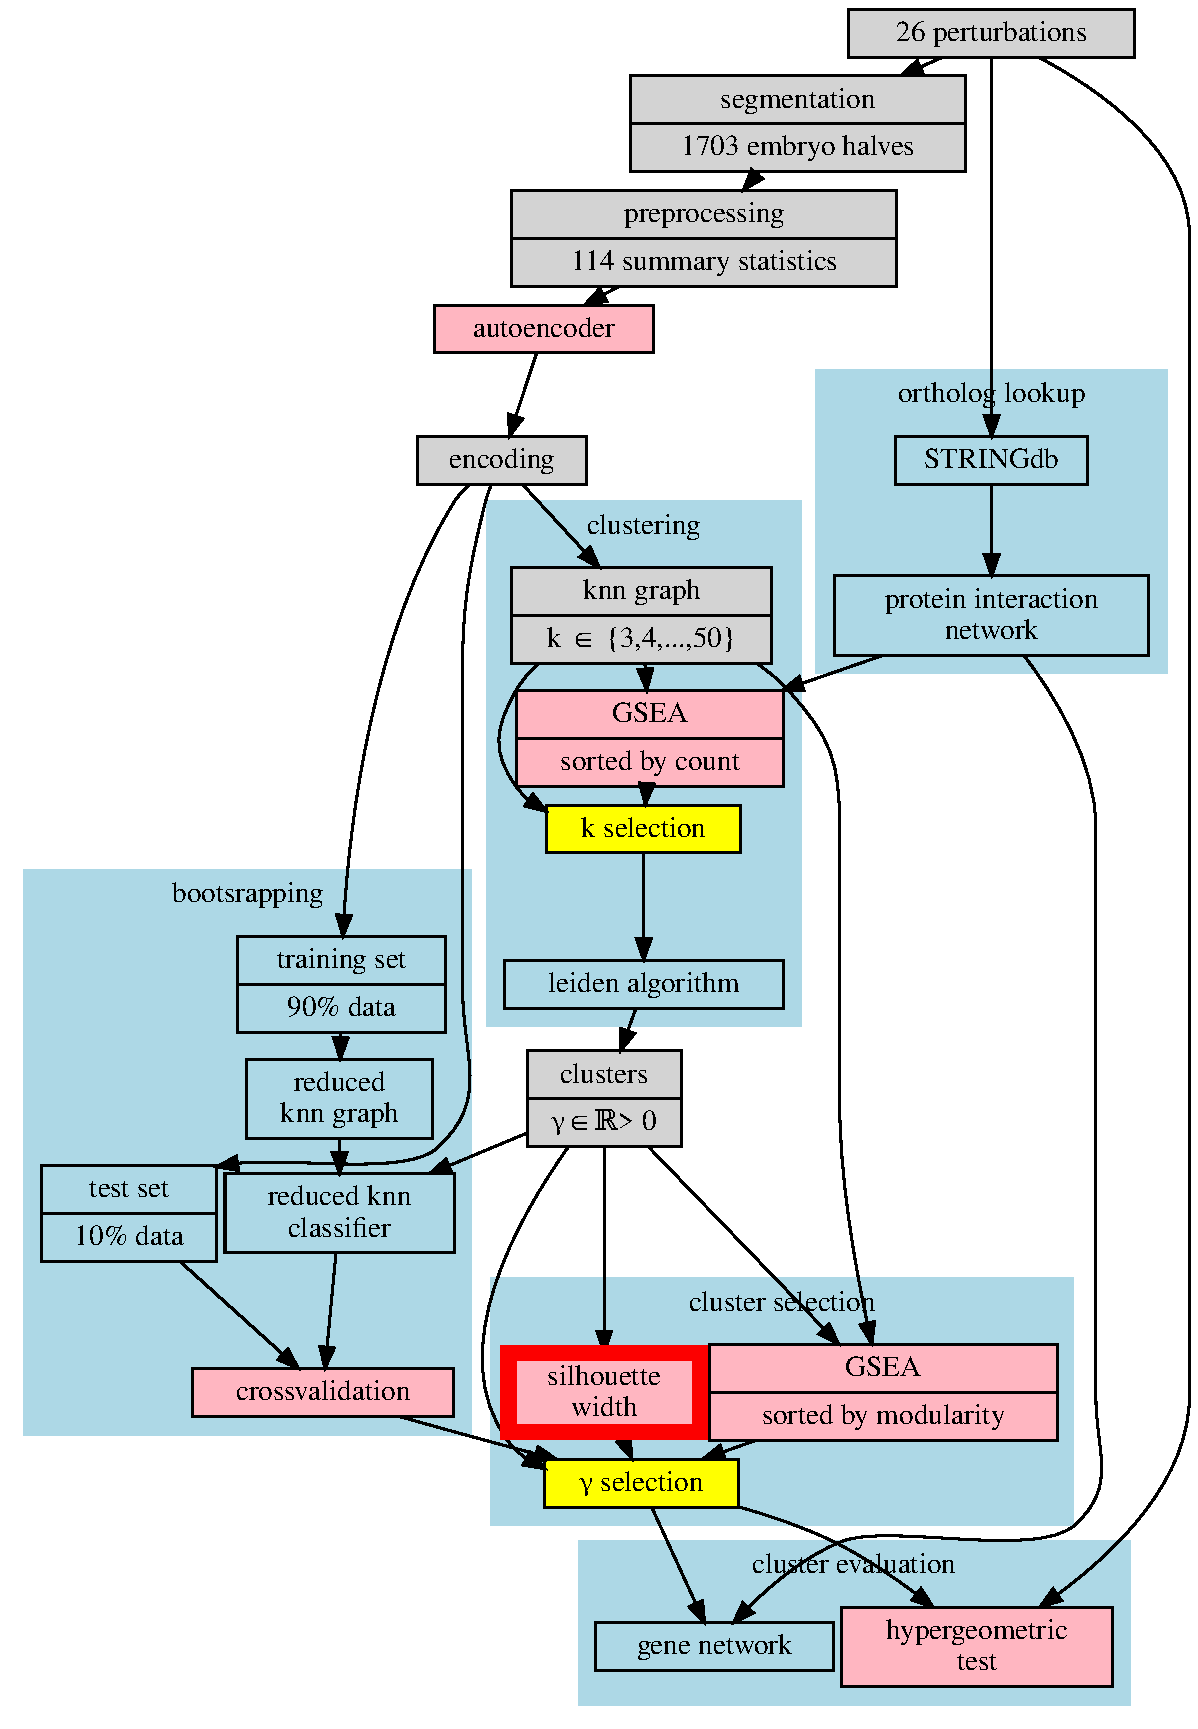
\includegraphics[width=\textwidth]{flowchart/sil.pdf}
		\end{column}
		\begin{column}{0.50\textwidth}
			Silhouette score gives the relative distance between points within a cluster compared to distance between points in different clusters. 
		\end{column}
	\end{columns}
}

\frame{
	\frametitle{}
	\begin{columns}
		\begin{column}{0.50\textwidth}
			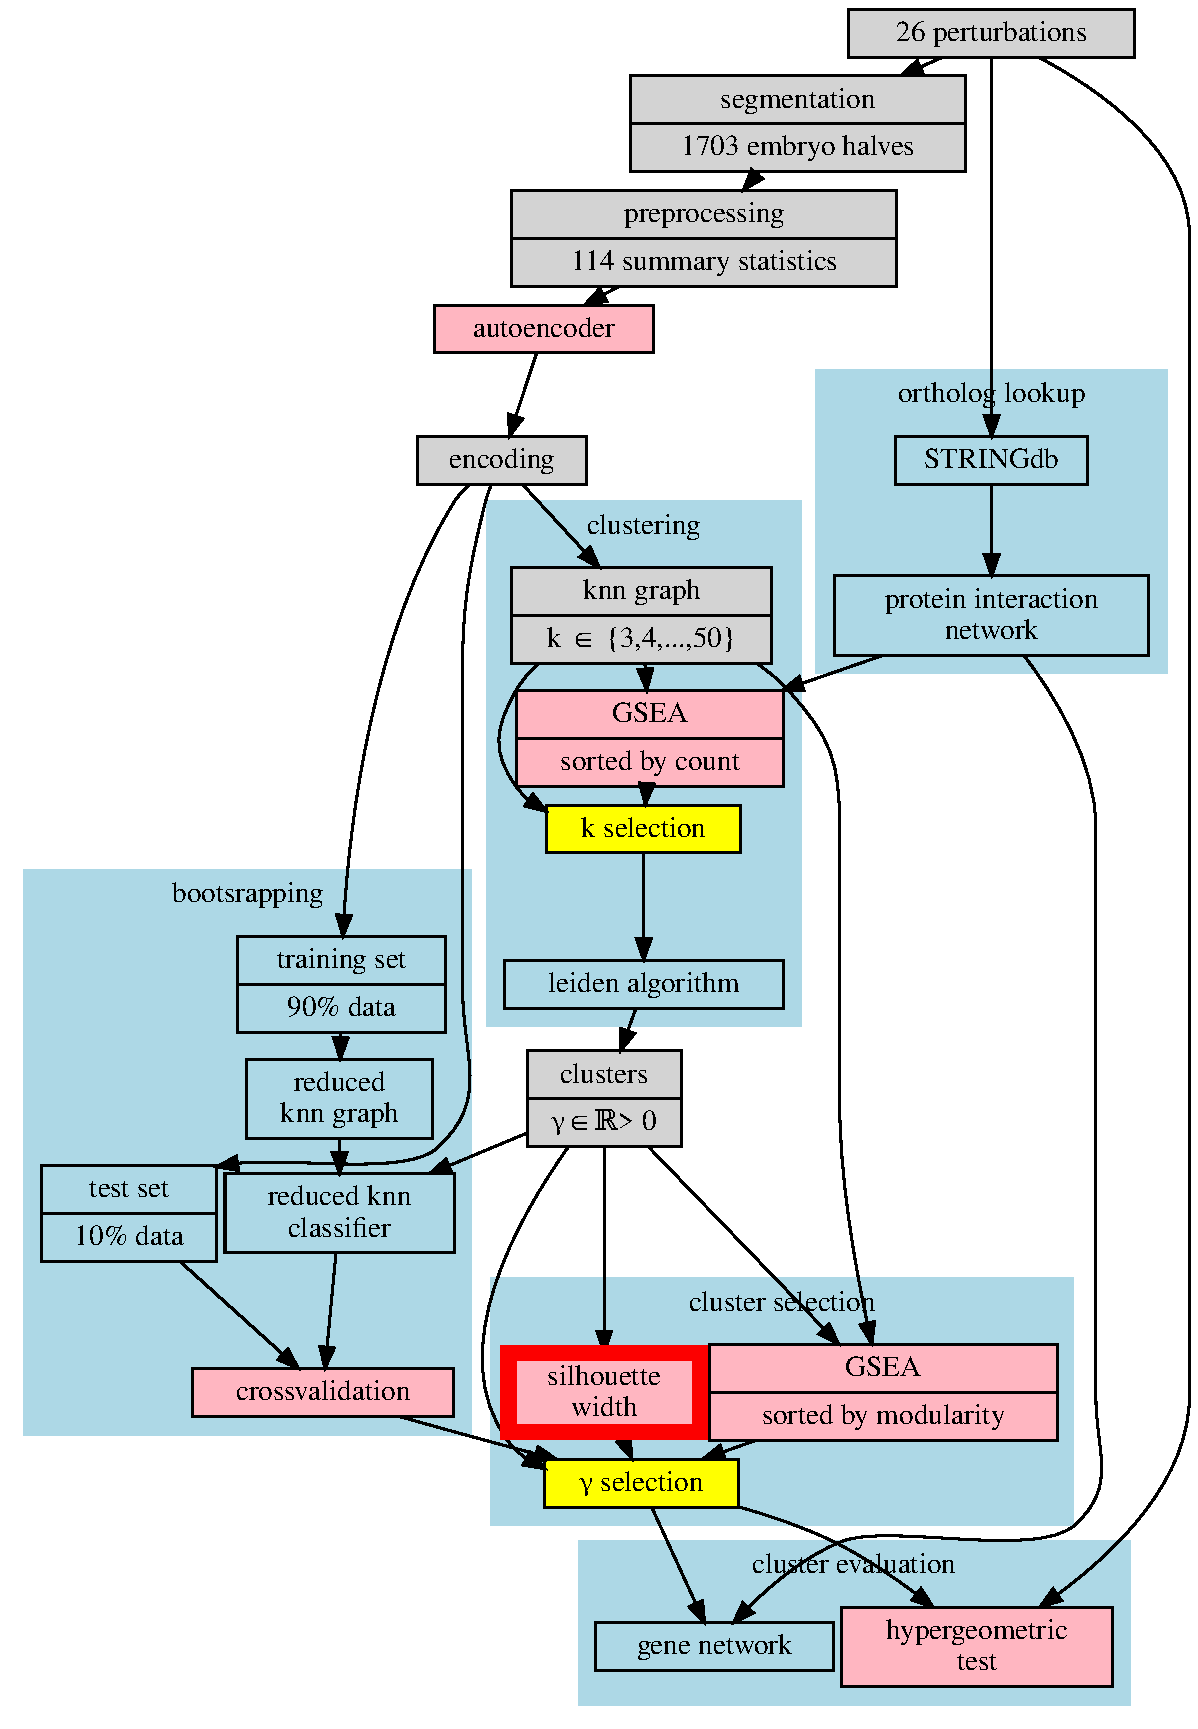
\includegraphics[width=\textwidth]{flowchart/sil.pdf}
		\end{column}
		\begin{column}{0.50\textwidth}
			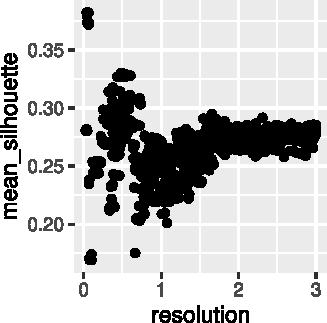
\includegraphics[width=0.5\textwidth]{sil.pdf}
			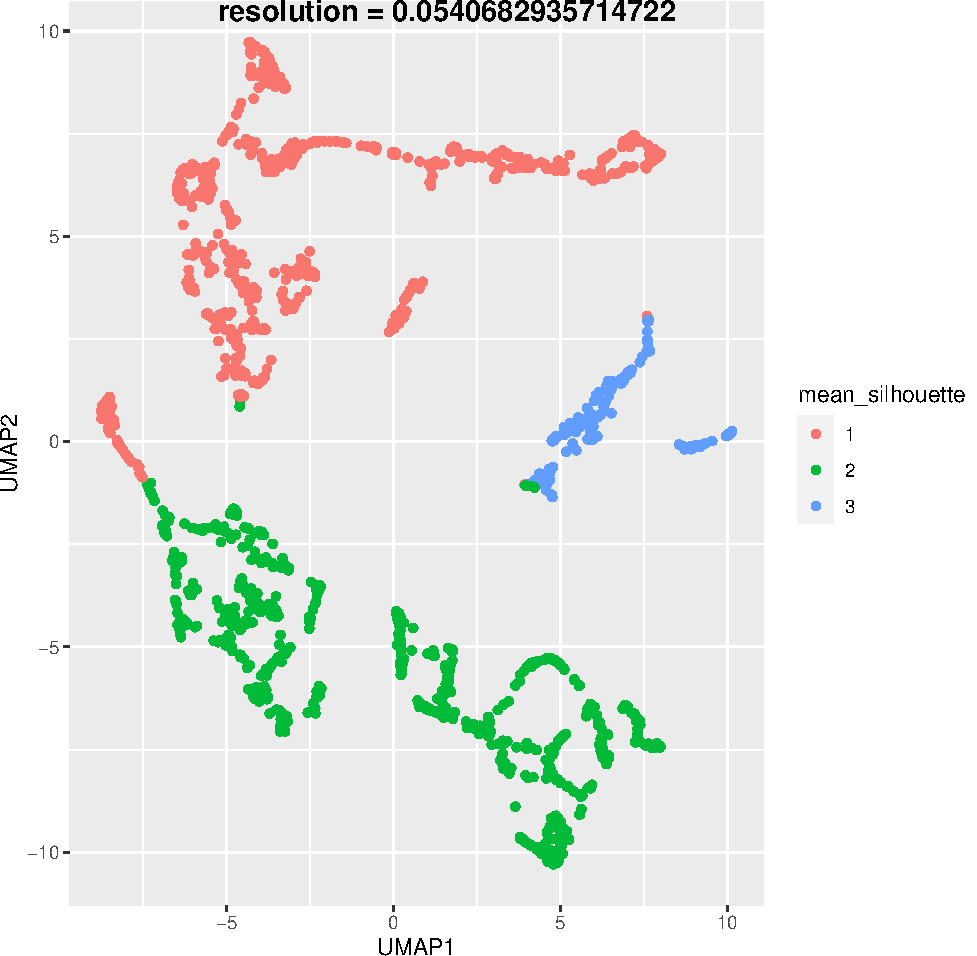
\includegraphics[width=\textwidth]{umap_sil.pdf}
		\end{column}
	\end{columns}
}

\frame{
	\frametitle{}
	\begin{columns}
		\begin{column}{0.50\textwidth}
			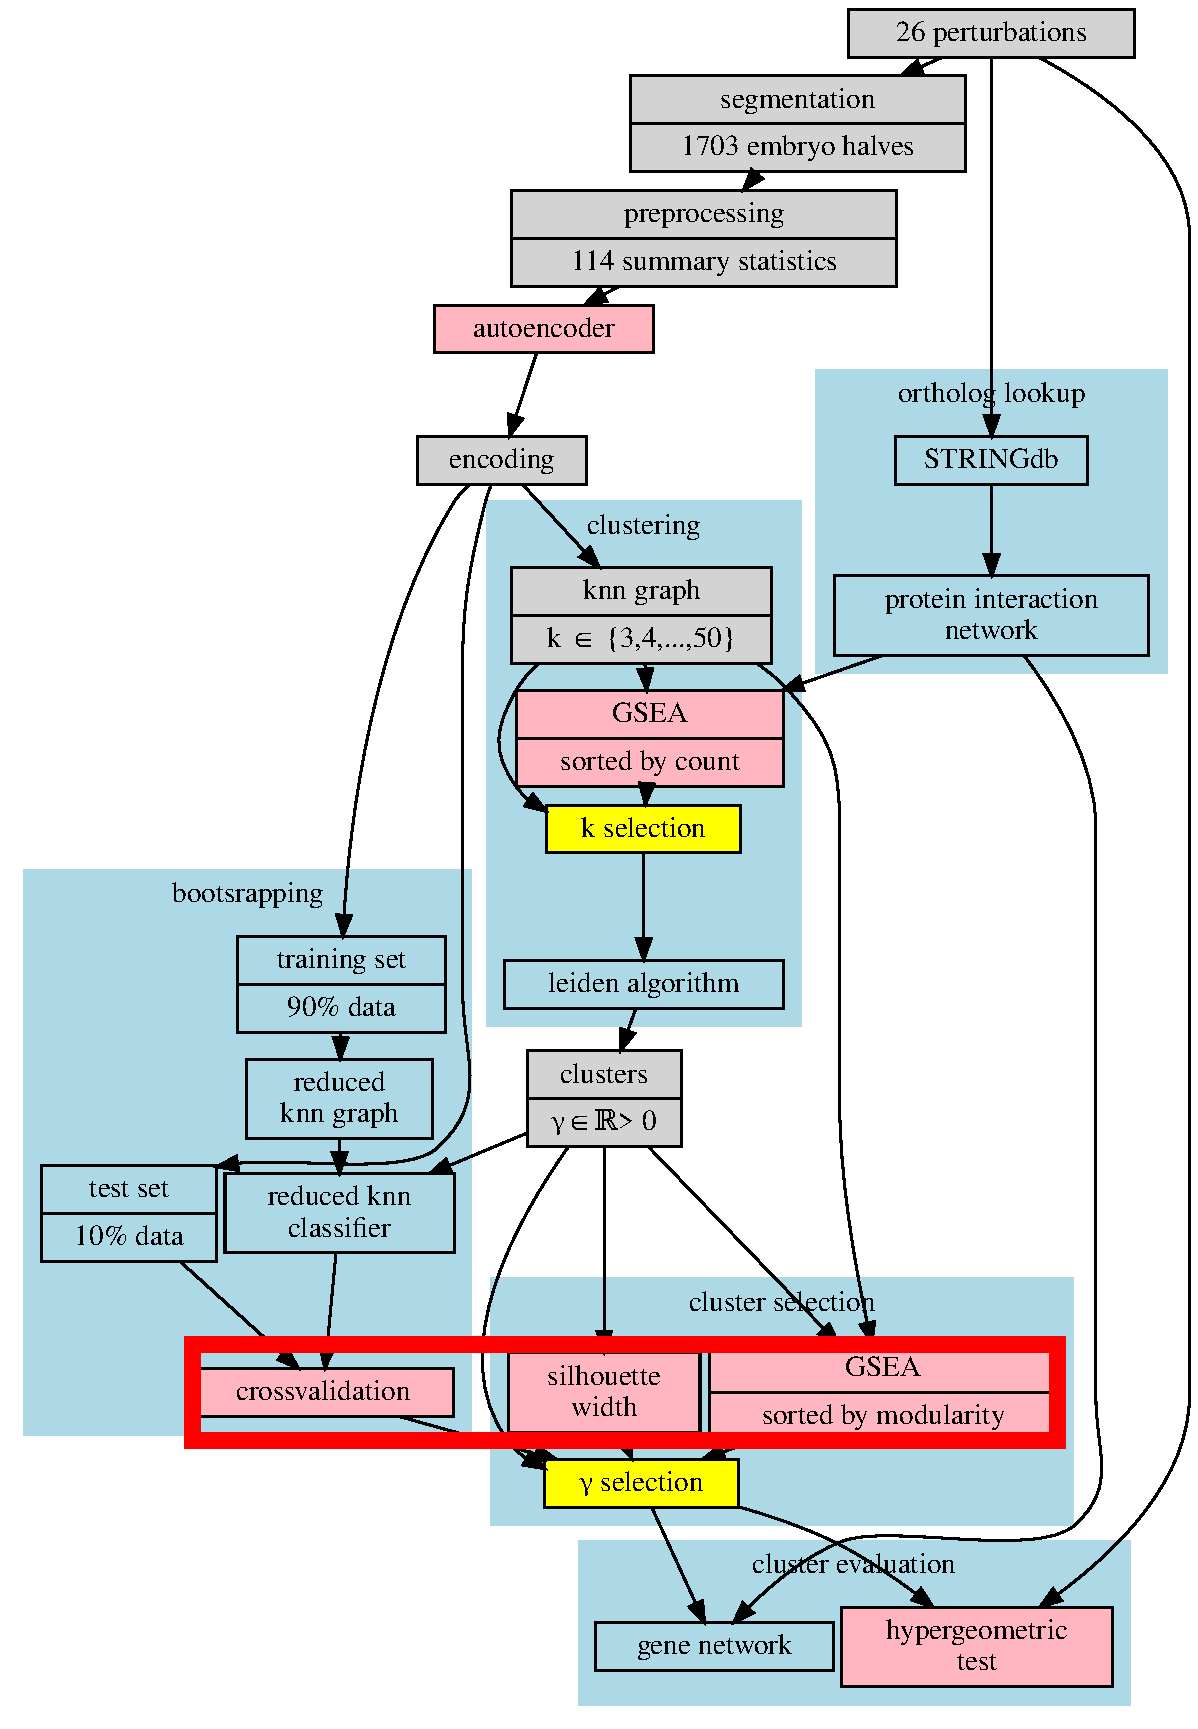
\includegraphics[width=\textwidth]{flowchart/ressel.pdf}
		\end{column}
		\begin{column}{0.50\textwidth}
			Because there was no clear best metric, I calculated a combined score from $ ES \times recall \times silhouette width \times -log_2 error $.
		\end{column}
	\end{columns}
}

\frame{
	\frametitle{}
	\begin{columns}
		\begin{column}{0.50\textwidth}
			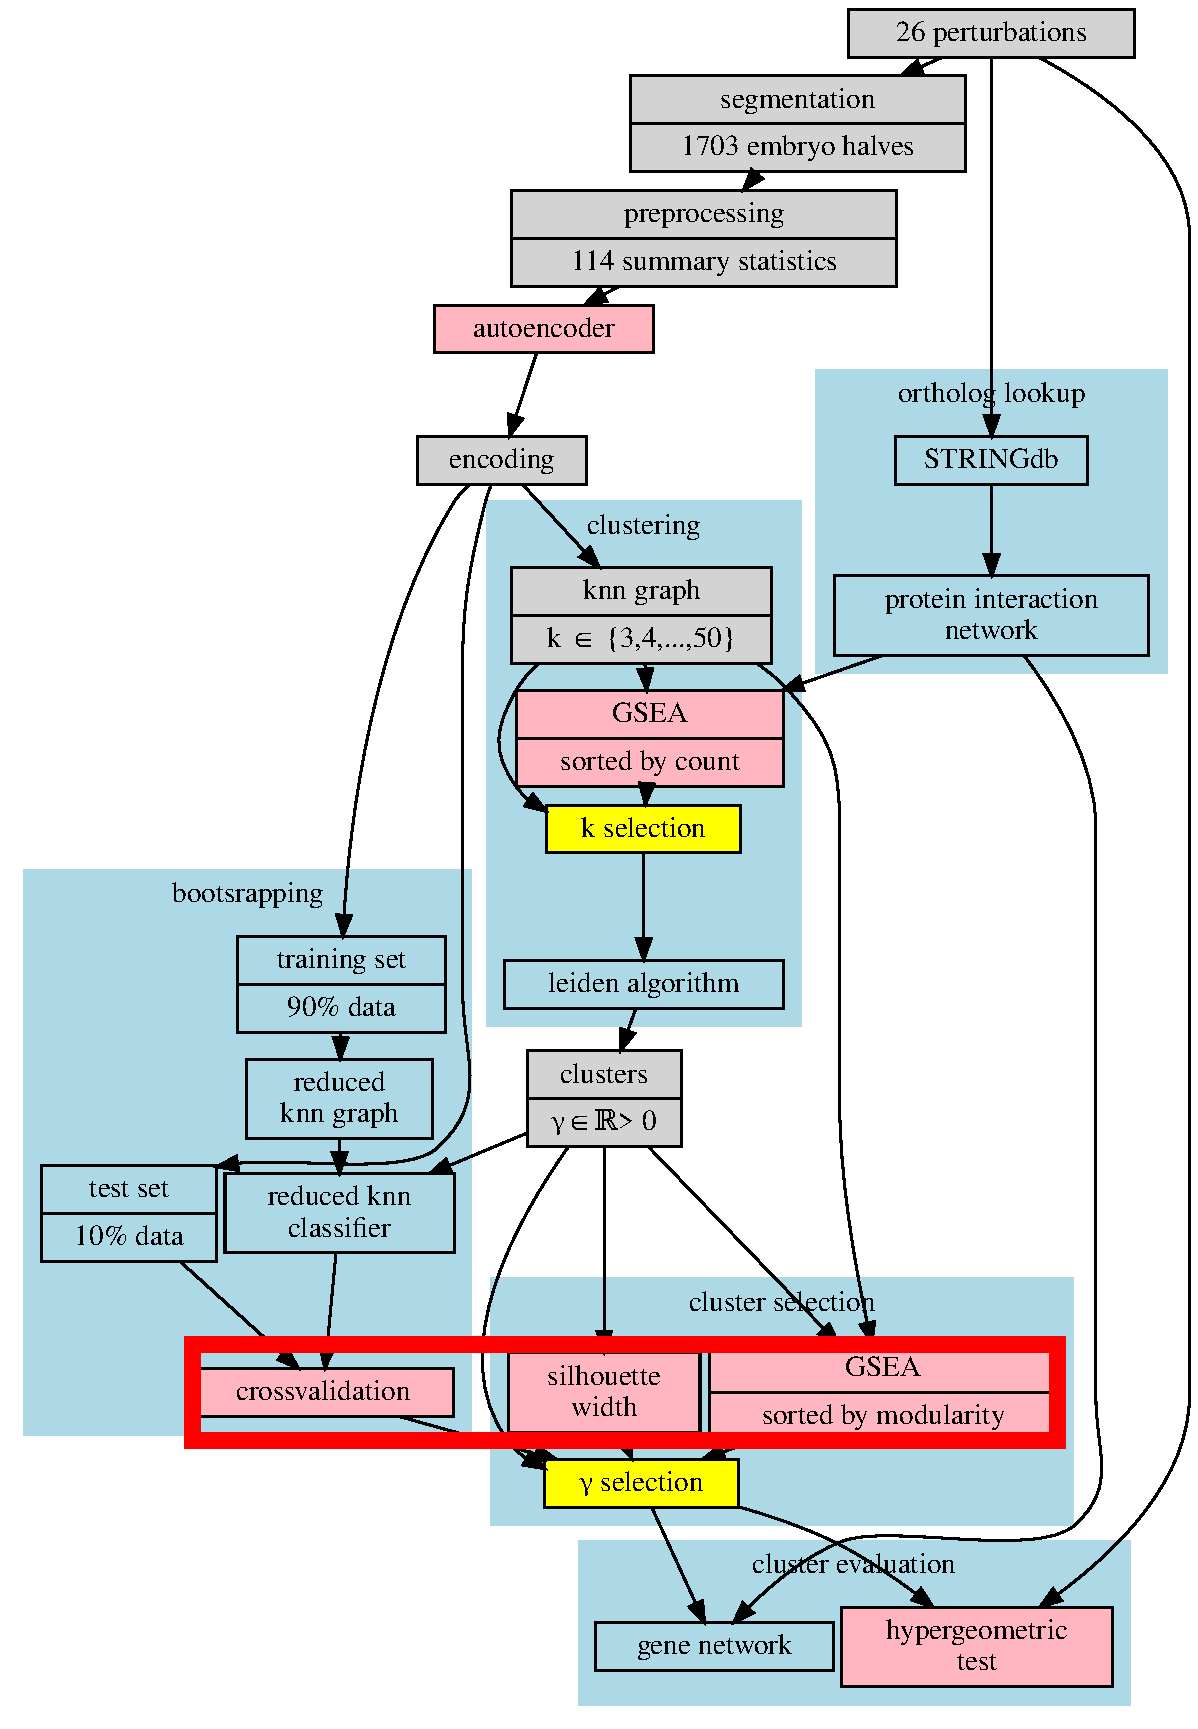
\includegraphics[width=\textwidth]{flowchart/ressel.pdf}
		\end{column}
		\begin{column}{0.50\textwidth}
			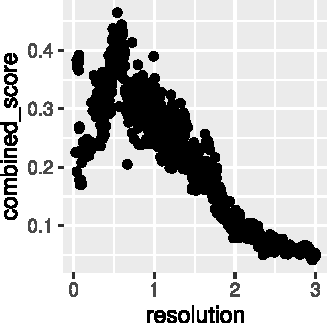
\includegraphics[width=0.5\textwidth]{combined.pdf}
			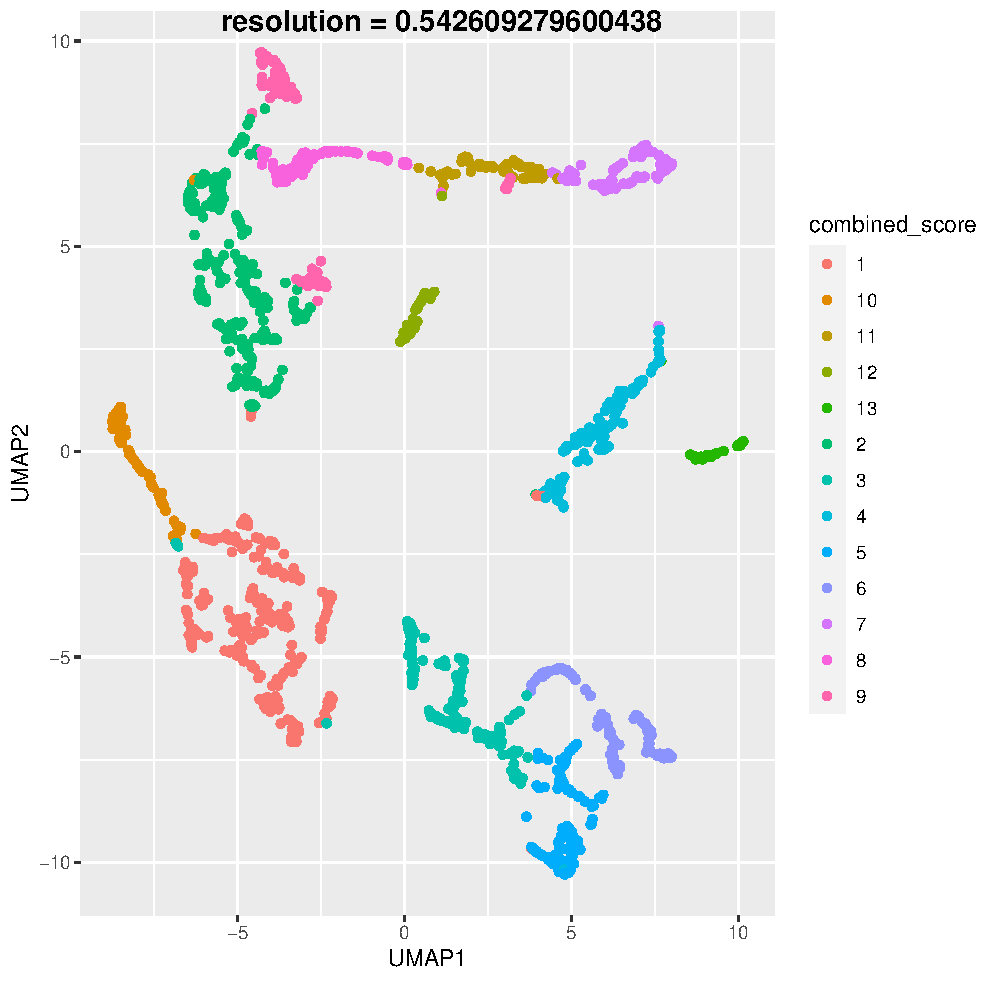
\includegraphics[width=\textwidth]{umap_combined.pdf}
		\end{column}
	\end{columns}
}

\frame{
	\frametitle{}
	\begin{columns}
		\begin{column}{0.50\textwidth}
			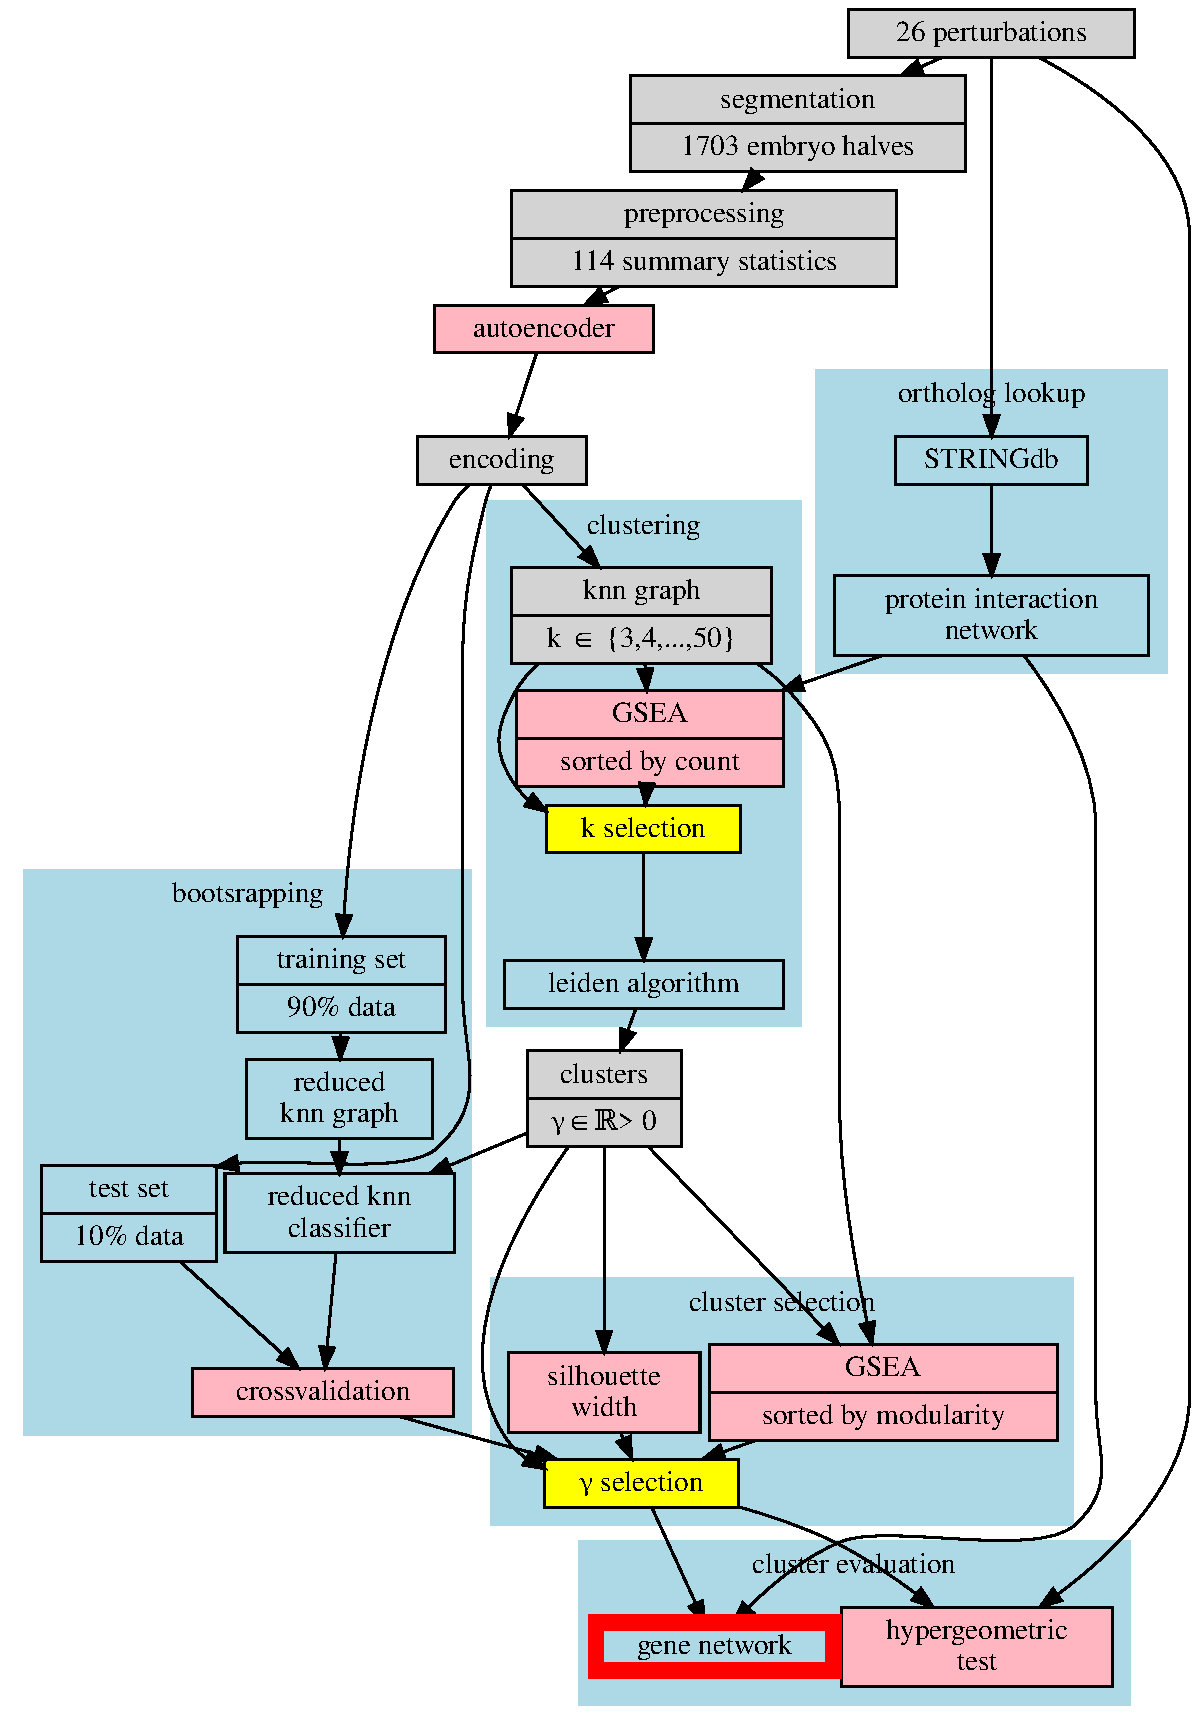
\includegraphics[width=\textwidth]{flowchart/gene.pdf}
		\end{column}
		\begin{column}{0.50\textwidth}
			I constructed a network using the top 5 modularity values for each gene.
		\end{column}
	\end{columns}
}


\frame{
	\frametitle{}
	\begin{columns}
		\begin{column}{0.50\textwidth}
			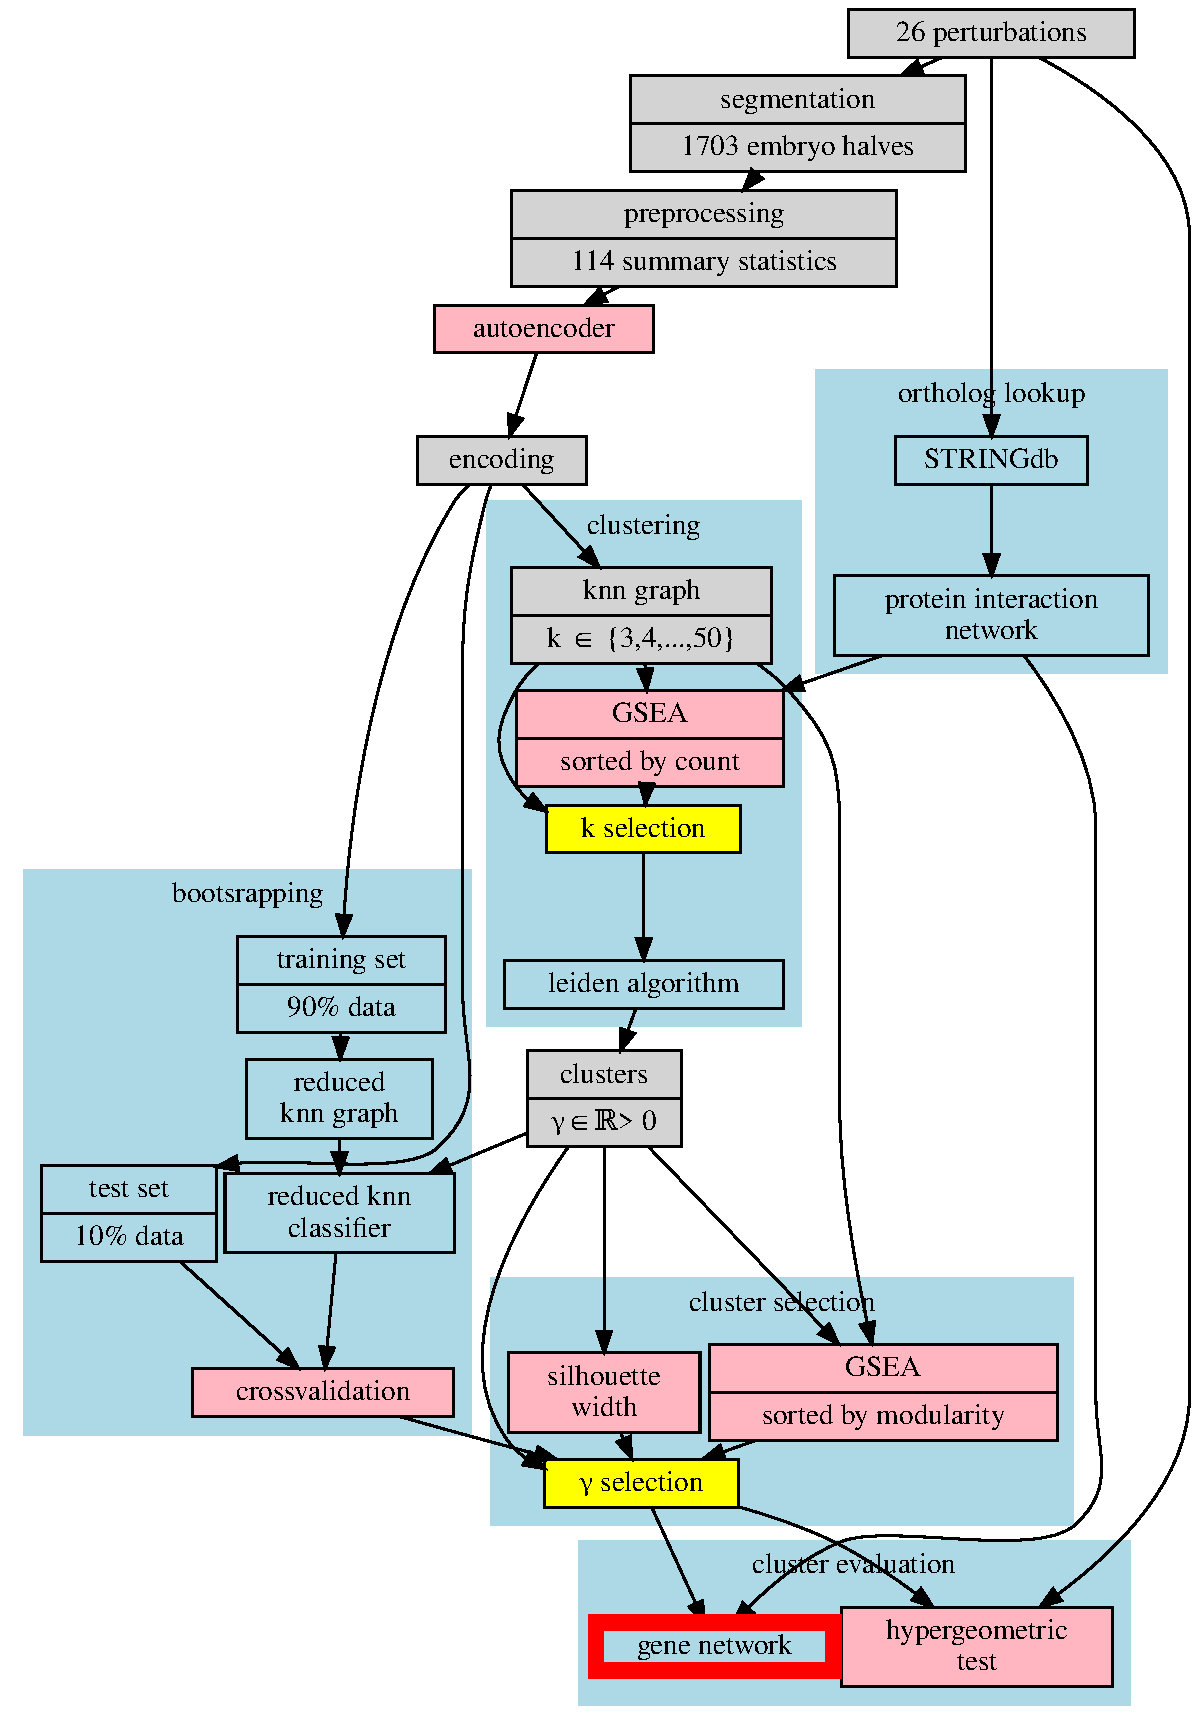
\includegraphics[width=\textwidth]{flowchart/gene.pdf}
		\end{column}
		\begin{column}{0.60\textwidth}
			\includegraphics[width=\textwidth]{gene_network_cropped.pdf}
		\end{column}
	\end{columns}
}

\frame{
	\frametitle{}
	\begin{columns}
		\begin{column}{0.50\textwidth}
			\includegraphics[width=\textwidth]{flowchart/hyper.pdf}
		\end{column}
		\begin{column}{0.50\textwidth}
			For each cluster I performed hypergeometric tests for enrichment of embryos in each treatment and enrichment of experimenter-identified phenotypes. 
		\end{column}
	\end{columns}
}

\frame{
	\frametitle{}
	\begin{columns}
		\begin{column}{0.50\textwidth}
			\includegraphics[width=\textwidth]{flowchart/hyper.pdf}
		\end{column}
		\begin{column}{0.80\textwidth}
			\includegraphics[width=\textwidth]{hyper.pdf}
		\end{column}
	\end{columns}
}

\end{document}
		
